\chapter{Plugins}%
\label{cha:plugins}

There are realtime effects -- these are the most useful and probably all you will ever need -- and rendered effects.
The rendered effects are discussed separately in the \nameref{sec:rendered_effects}  section.
Effect plugins modify the track when played, according to how they are set, with no permanent storage of the output except when the project is rendered. There are many Plugins in \CGG{} Infinity which are actually quite easy to use just by experimenting with them. The plugins are shown and selected from the \textit{Resources window} (figure~\ref{fig:video-plugins}). They are described in more detail later.

\begin{figure}[htpb]
    \centering
    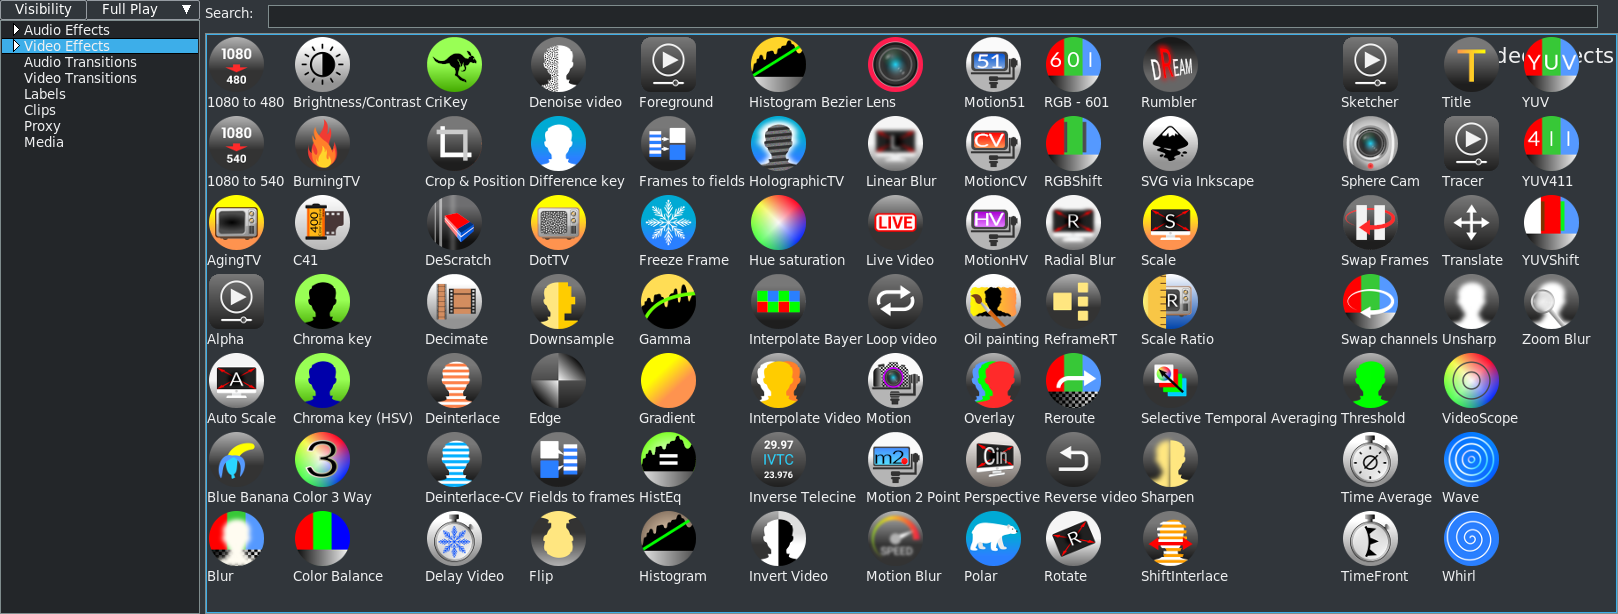
\includegraphics[width=1.0\linewidth]{video-plugins.png}
    \caption{Screencast of the native Video plugins in the default Cinfinity icon set.}
    \label{fig:video-plugins}
\end{figure}

There is a choice of plugin icons which can be displayed.

In \texttt{Settings$\rightarrow$ Preferences$\rightarrow$ Appearance} tab, there is a pulldown for \textit{Plugin icons} where the user can choose between the \textit{original} icons, \textit{regular} or \textit{smoother}, \textit{cinfinity}\protect\footnote{Cinfinity /2 icon set is credited to Sam - Creative Common By -- \url{https://creativhecommons.org/licenses/by/3.0/}} -- the default modernized set, or \textit{cinfinity2} (figure~\ref{fig:audio-plugins}).

Note that when you change the plugin icons, your session will automatically save the backup, stop, restart, and reload (figure~\ref{fig:plugin-icons}).

\begin{figure}[htpb]
    \centering
    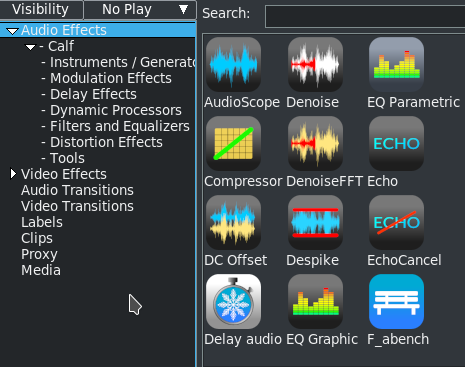
\includegraphics[width=0.6\linewidth]{audio-plugins.png}
    \caption{Cinfinity2 audio plugins}
    \label{fig:audio-plugins}
\end{figure}

\begin{figure}[htpb]
    \centering
    \begin{tikzpicture}[scale=1, transform shape]
    \node (img1) [yshift=0cm, xshift=0cm, rotate=0] {\includegraphics[width=0.5\linewidth]{plugin-icons.png}};
    \node [yshift=-6mm, xshift=-1cm,anchor=east] at (img1.north west) (Preferences) {Preferences Window};
    \node [yshift=-14mm, xshift=-1cm,anchor=east] at (img1.north west) (Tab) {Tab section};
    \node [yshift=-34mm, xshift=-1cm,anchor=east] at (img1.north west) (Icon) {Plugin icon choices};
    \draw [->, line width=1mm] (Preferences) edge  ([yshift=-6mm] img1.north west);
    \draw [->, line width=1mm] (Tab) edge  ([yshift=-14mm] img1.north west);
    \draw [->, line width=1mm] (Icon) edge    ([yshift=-34mm] img1.north west);
    \end{tikzpicture}
    \caption{Screencast showing the screen to change your plugin icons set}
    \label{fig:plugin-icons}
\end{figure}

\section{How to Use Plugins}%
\label{sec:how_use_plugins}

\textit{Realtime} effect plugins are listed in the Resources window as \textit{Audio} Effects and \textit{Video} Effects. Effect plugins are used by dragging them from the Resources window onto an audio track if it is an audio effect or video track if it is a video effect. You will see a colored bar appear beneath the track with the plugin name on it. If there is data on the destination track, the effect is applied to the entire track, unless a region of the track is selected in which case the effect is pasted into that region only. If there is no data on the track the effect is not added.

Plugins are layered under the track they apply to. When dragging more than one effect onto a track, you will see the effects layering from \textit{top to bottom}, on the bottom of that track. When the track is played back, effects are processed from \textit{top to bottom}. The output of the top effect becomes the input of the bottom effect and so on.

Instead of dragging from the Resources window, effects may be applied to a track via a popup menu. Right click on a track and select \textit{Attach effect} from the popup. The attach effect dialog gives you more capability than just dragging and dropping. For example, the attach effect dialog lets you attach two more types of effects: \textit{shared effects} and \textit{shared tracks} which are explained in a later section. Select a plugin from the Plugins column and hit the green colored checkmark under the plugins column to attach it. The result is the same as if the effect was dragged from the Resources window.

After attaching an effect to a track, it often needs to be configured. There are two ways to get to the configuration controls. Click on the magnifying glass symbol on the right side of the effect bar -- this is the middle symbol on the bar as you can see in the picture below. Alternatively, you can right click on the effect bar to bring up the effect popup which has a \textit{Show} option. Either method causes the GUI for the effect to appear in a separate window. There will not be a popup if the plugin has no GUI.


Besides the magnifying glass, for Show Controls, on the effect colored bar beneath the track, there are two more symbols.

\begin{wrapfigure}[2]{r}{0.3\linewidth}
    \vspace{-3ex}
    \centering
    
\includegraphics[width=0.7\linewidth]{button-options.png}
\end{wrapfigure}

The rightmost knob is used to Turn Off/Turn On the effect where the default is On. This is useful to easily see that the plugin is doing what you expect. The leftmost symbol that looks like a gear is for \textit{Preset Edit} and its usage is described in the section \nameref{sec:saved_plugin_preset}.

\section{Editing Effects}%
\label{sec:editing_effects}

Many operations exist for manipulating effects once they are on the timeline. Because mixing effects and media is quite complex, the methods used in editing effects are not as concise as cutting and pasting. Some of the editing happens by dragging in/out points, some of the editing happens through popup menus, and some of it happens by dragging effects.

When enabled, which is the default, and you edit tracks, the effects follow the editing decisions. If you cut from a track, the effect shrinks. If you drag edit in/out points, the effect changes length. This behavior can be disabled by selecting \texttt{Settings$\rightarrow$ Preferences$\rightarrow$ Interface tab$\rightarrow$ Editing section}, see figure~\ref{fig:editing-effects}.

\begin{figure}[htpb]
    \centering
    \includegraphics[width=0.9\linewidth]{editing-effects.png}
    \caption{Screencast of the native Video plugins in the default Cinfinity icon set.}
    \label{fig:editing-effects}
\end{figure}

To edit effects, you can move the timeline cursor over the effect borders until it changes to a resize left or resize right icon. In this state, if you drag the end of the effect, it performs an edit just like dragging an edit edge. The five editing behaviors of track trimming apply to effect trimming and they are bound to the mouse buttons that you set in interface preferences as shown in the previous screencast. \textit{Trimming} simply means changes the duration dragging the edges.

When you perform a trim edit on an effect, the effect boundary is moved by dragging it. Unlike track editing, the effect has no source length. You can extend the end of an effect as much as you want. Also unlike track editing, the starting position of the drag operation does not bind the edit decision to media. The media the effect is bound to does not follow effect edits. Other effects, however, do follow editing decisions made on an effect. You can disable effects from being subject to the edit decisions by using the pulldown Settings and toggling off Edit effects. If you drag the end of an effect which is lined up to effects on other tracks, the effects on the other tracks will be edited while the media stays the same. When you drag an effect in from the Resources window you can insert the effect in the portion of the row unoccupied by the trimming operation. In some cases you will want a trimming operation to change only one row of effects. This can be achieved by first positioning the insertion point on the start or end of the effect. Then press the shift key while beginning the trimming operation. This causes the operation to change only one row of effects.

You can move effects up or down. Every track can have a stack of effects under it. By moving an effect up or down you change the order in which effects are processed in the stack. Go to an effect and right click to bring up the effect menu. The \textit{Move up} and \textit{Move down} options move the effect up or down. When you are moving effects up or down, be aware that if they are shared as shared effects, any references will be pointing to a different effect after the move operation.

Finally, there is dragging of effects. Dragging effects works just like dragging edits. You must select the arrow in the main window transport buttons line to enter drag and drop mode before dragging effects. Dragging a plugin causes a highlight outline to be drawn over a targetable timeline region, and the plugin can be re-positioned into any plugin track.  The effects snap to media boundaries, effect boundaries, and tracks. If you drag a reference to a shared effect, the reference may point to the wrong effect afterwards.  It is recommended that you re-construct shared effect track references.

Figure~\ref{fig:drag-effect} showing 5 plugins, two still plugin, two have already been dragged and the \textit{Color 3 Way} in the process of being dragged. Note the gold-colored arrow which enables allow \textit{drag and drop} editing mode.

\begin{figure}[htpb]
    \centering
    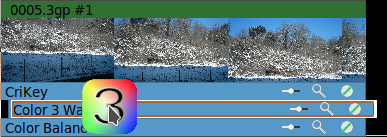
\includegraphics[width=0.7\linewidth]{drag-effect.png}
    \caption{Dragging the Color 3 way effect}
    \label{fig:drag-effect}
\end{figure}

\section{Shared Effects and Shared Tracks}%
\label{sec:shared_effect_tracks}

Two other effect types available in the Attach Effect dialog are \textit{Shared effects} and \textit{Shared tracks}. In the case of a shared effect, the following conditions must be true:

\begin{itemize}[noitemsep]
    \item There must be other effects in the timeline.
    \item The other effects must be of the same type as the track you are attaching an effect to. That is for audio tracks, effect must be audio and for video tracks, effect must be a video effect.
    \item The insertion point or selected region must start inside the other effects.
\end{itemize}

In the case of a shared track, there must be another track on the timeline of the same type as the track you are applying an effect to. If you right clicked on a video track to attach an effect, there will not be anything in the shared tracks column if no other video track exists. The same applies equally to audio tracks in that another audio track must exist. Shared tracks are often used as layers for titles, curves and keyframes.

If shared effects or shared tracks are available, they appear in the shared effects and shared tracks columns when you used the \textit{Attach effect} option (RMB on a track). When the green colored checkmark is clicked OK, anything highlighted in the column is attached under the current track.

Shared effects and shared tracks allow very unique things to be done. In the case of a shared effect, the shared effect is treated like a copy of the original effect, except that in the shared effect the GUI can not be brought up. All configuration of the shared effect is determined by the GUI of the original effect and only the GUI of the original effect can be brought up.

When a shared effect is played back, it is processed just like a normal effect except the configuration is copied from the original effect. Some effects detect when they are being shared. These effects determine what tracks are sharing them and either mix the two tracks together or use one track to stage some value.

When an original track has a shared track as one of its effects, the shared track itself is used as a \textit{realtime} effect. This is more commonly known as \textit{bouncing tracks} but \CGG{} achieves the same operation by attaching shared tracks. The fade and any effects in the shared track are applied to the original track. Once the shared track has processed the data, the original track performs any effects which come below the shared track and then composites it on the output.

In order to prevent the shared track from mixing the same data as the original track on the output, enable the output \texttt{mute} toggle in the patchbay next to each track for which you do not want to mix on the output. If you are making a video and you do want the shared track to composite the original track's data on the output a second time, the video from the shared track would always appear under the video from the original track, regardless of whether it was on top of the original track. This is because shared tracks are composited in order of their attachment. Since it is part of the original track it has to be composited before the original track is.

\section{Saved Plugin Presets}%
\label{sec:saved_plugin_preset}

\textit{Presets} and \textit{Factory Presets} for Plugin settings are now combined with the Preset Keyframe Parameters allowing you to choose, apply, delete, and edit your own Presets which can then be easily saved in the file \texttt{\$HOME/.bcast5/Cinelerra\_presets}. In addition to your own saved presets, there are automatically available Factory presets for some plugins, for example the Lens video plugin. The Factory presets are preceded by an asterisk (*) and can not be modified permanently.

\begin{wrapfigure}[4]{r}{0.3\linewidth}
    \vspace{-2ex}
    \centering
    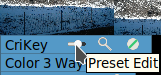
\includegraphics[width=0.7\linewidth]{preset.png}
\end{wrapfigure}
Note that using this is directly changing a keyframe object so you will only want to modify parameters you are familiar with. Most of the data is obvious and safe to change.

A Presets button on the plugin bar to the left of the Controls and On/Off button allows for quick access to this feature. The symbol resembles a slider (figure~\ref{fig:preset02}).

\begin{figure}[htpb]
    \centering
    \begin{tikzpicture}[scale=1, transform shape]
    \node (img1) [yshift=0cm, xshift=0cm, rotate=0] {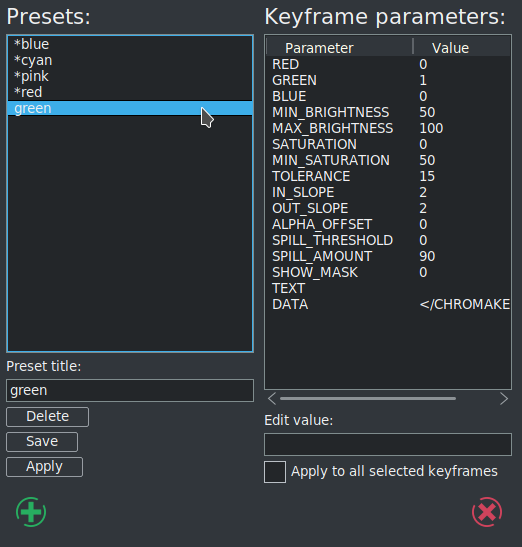
\includegraphics[width=0.6\linewidth]{preset02.png}};
    \node [yshift=-20mm, xshift=-1cm,anchor=east] at (img1.north west) (Green) {A user preset Green};
    \node [yshift=-67mm, xshift=-1cm,anchor=south east,text width=10em, inner ysep=-3mm] at (img1.north west) (Textbox) {Textbox to type in the title for the chosen preset or name for a new preset.};
    \node [yshift=-79mm, xshift=-1cm,anchor=north east,text width=10em,inner ysep=-3mm] at (img1.north west) (Save) {Use the Delete, Save or Apply button for operation.};
    \draw [->, line width=1mm] (Green) edge  ([yshift=-20mm] img1.north west);
    \draw [->, line width=1mm] (Textbox.south east) --  ([yshift=-67mm] img1.north west);
    \draw [->, line width=1mm] (Save.north east) --    ([yshift=-79mm] img1.north west);
    \end{tikzpicture}
    \caption{Screencast shows 4 Factory presets as preceded by an *.}
    \label{fig:preset02}
\end{figure}

\section{Some specific details concerning Plugins}%
\label{sec:specific_details_plugins}

These next few sections explain some details about the plugins that are not directly related to actually using them but help to work with them.

\subsection{How to see short Description of a Plugin}%
\label{sub:short_description_plugin}

To get a short one or a few lines description of a plugin, mouse over that plugin in the Resources window and a popup appears. You can disable the popup by right-clicking and choosing \textit{Info Off} (shortcut "i"). And again enable it with \textit{Info On}. Some of the plugins may not have any description included. An example screenshot is next (figure~\ref{fig:info-effect}).

\begin{figure}[htpb]
    \centering
    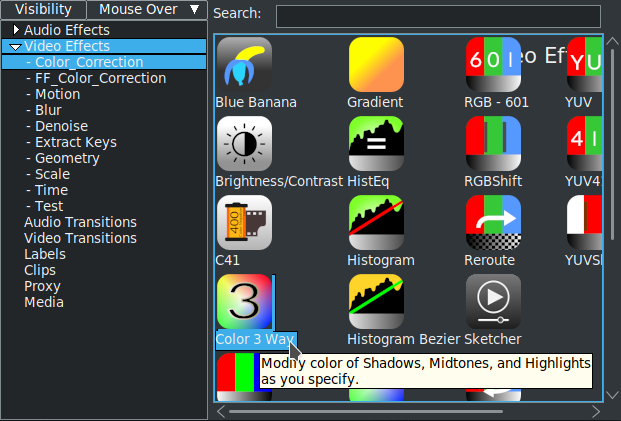
\includegraphics[width=0.8\linewidth]{info-effect.png}
    \caption{Effect Info for Color 3 Way}
    \label{fig:info-effect}
\end{figure}

\subsection{Delete Plugins to save Resources Space or make them Unavailable}%
\label{sub:delete_plugin_resouces_unavaible}

Maybe you just don't ever use certain plugins or would prefer to only find the ones that are useful to you. To save space in the Resources Window so you don't have to scroll to find the plugins you want as much, a feature to delete others is available. If you have a System install, you will have to be root for this function to be usable. The plugins will be permanently deleted, but only until you rebuild or download a new set of \CGG{} binaries. To delete a plugin, highlight the plugin you no longer want in the Resources window then press Ctrl-Shift-delete. A small window will come up allowing you to change your mind and red-X out or check-OK to remove plugin. This feature may come in handy if you have personnel working on media for you and you only want them to exercise certain functions. Or maybe you can't remember which is the good \textit{deinterlace} plugin out of the available five or so and want to delete the extras so as not to be confused. The ffmpeg, \textit{ladspa}, and \textit{lv2} plugins can not be deleted in this manner but, of course, you can always turn them off from view by clicking on \textit{Visibility} and unchecking them (figure~\ref{fig:remove-effect}).

\begin{figure}[htpb]
    \centering
    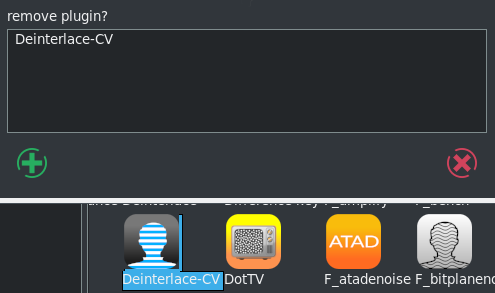
\includegraphics[width=0.6\linewidth]{remove-effect.png}
    \caption{Remove Deinterlace-CV plugin}
    \label{fig:remove-effect}
\end{figure}

\subsection{Updatable Icon Image Support}%
\label{sub:updatable_icon_image_support}

When running \CGG{} Infinity builtin icons are loaded before the
program starts. Png files in the path:\\
\texttt{<target\_directory>picon/picon\_set\_name}\\
are searched before the images loaded into memory. Override
\texttt{icon.png} files must be put into the path:\\
\texttt{<target\_directory>/picon/picon\_set\_name}\\
There are currently 4 sets of icons and their directory names are
\textit{cinfinity} (the default) and \textit{cinfinity2},
\textit{original} (the long-time original set), and
\textit{smoother} (generally was in use by some of the themes). An
example, to replace the cinfinity icon of Blue Banana with a red
apple instead, create your \texttt{.png} file as desired, and replace the
file in:\\
\texttt{<target\_directory>/bin/plugins/picon/cinfinity/bluebanana.png}.

For most User installs, the \texttt{<plugin\_name>.png} file will be located at:

\texttt{<cinlib\_path>/bin/plugins/picon/cinfinity} (or cinfinity2, original or smoother)

For some System installs, the files might be located at:

\texttt{/usr/lib/cin/plugins/picon/cinfinity}

(or cinfinity2, original or smoother -- ubuntu distros)

\texttt{/usr/lib64/cin/plugins/picon/cinfinity}

(or cinfinity2, original or smoother -- Leap distro)

\subsection{Details on where to put your own Plugin Icons}%
\label{sub:details_put_plugin_icons}

In order to make the icons available to all themes, which would thus be the default when no theme-specific icon is available, put the png file in the:

\texttt{<cinlib\_path>/bin/plugins/picon/cinfinity} (or cinfinity2, original or smoother)

The \CGG{} program looks for a plugin icon in two places:

\begin{enumerate}
    \item First, it tries to find a png file in \texttt{<cinlib>/plugins/picon/cinfinity}(2) or original, smoother directory.
    \item If there is no corresponding \texttt{.png} file for a plugin, the program uses a built-in default:
    \begin{itemize}
        \item ordinary video plugins use 3 vertical color bars as a default;
        \item ffmpeg plugins use the words \textit{FF} on yellow colored background as a default icon;
        \item audio and ladspa plugins use a green-colored audio wave for a default.
    \end{itemize}
\end{enumerate}
\begin{figure}[htpb]
    \centering
    \includegraphics[width=0.05\linewidth]{audio-default.png}
\end{figure}

Keep in mind these points for newly created plugin icons:

\begin{itemize}
    \item All included icon images become part of open source, in the public domain, and not proprietary.
    \item The preferred format is $52 \times 52$, $8\,bit$ /color RGB or RGBA, non-interlaced.
    \item Since plugin icons are used by different themes, it is recommended that a \textit{transparent background} be used. Otherwise some color background that looks good for one theme may not for another.
    \item In order to test a new icon, you have to have write permission in the: \\
    \texttt{<cinlib\_path>/plugins} directory so you may have to become the root user to copy the \texttt{.png} file to the correct location.
    \item If there is currently no theme-specific \texttt{.png} files present, it may be necessary to first create the theme directory in \texttt{<cinlib\_path>plugins} as \texttt{<theme\_name>} in order to put the \texttt{.png} files in that subdirectory.
    \item Make sure that the \textit{ownership} and file \textit{permissions} match the existing directory and files.
    \item All ffmpeg icons must begin with \texttt{ff\_<plugin\_name>.png} (Resources window title will still be F\_\dots)
    \item For ladspa, check in the \texttt{<cin\_config>} directory (\texttt{\$HOME/.bcast5} normally) and look for the text file \texttt{\$HOME/.bcast5/ladspa\_plugins\dots} for the names of the ladspa libraries which correspond to plugin names where the needed name is the basename of the \texttt{.so} file.
        For example \texttt{pha\-sers\_1217.so} would need to have a \texttt{phasers\_1217.png} file. There may be multiple plugins in a single “so” file which means that you can only have 1 icon to represent all of the plugins in that file; again as in phasers.
    \item Once you have placed the .png file in the correct spot, you will have to restart \CGG{} to test it.
    \item To submit your \texttt{.png} file for inclusion into \CGG{} Infinity for all to enjoy, it is best to upload it to any datafilehost and notify the community via email with any informative documentation.
\end{itemize}

\subsection{Example of new Plugin Icon Testing}%
\label{sub:example_plugin_icon_testing}

For a simple test just copy an existing \texttt{<plugin\_name>.png} file into the cinfinity directory with the name \texttt{bluebanana.png} to write over the existing file. This icon will now show up in \CGG{} and still execute the Blue Banana function.

For an ffmpeg plugin, create \texttt{ff\_loop.png} and copy it to: \\
\texttt{<cinlib\_path>/plugins/picon/original}. This icon will show up in \CGG{} if original is selected and execute the \textit{F\_loop} function.

For a ladspa plugin, the text line in \texttt{\$HOME/.bcast5/ladspa\_plugins}$\dots$ as seen below:
2 \texttt{am\_pitchshift\_1433.so} \\
\texttt{AM pitchshifter} $1504922321\, 0\, 1\, 0\, 0\, 1\, 0\, 1\, 0\, 1\, 0\, 0$ indicates that you would create the icon: \\ \texttt{<cinlib\_path>/plugins/picon/cinfinity/am\_pitchshift\_1433.png} \\
For your own personal plugins, you can create a directory on your system and put any plugin png files you like into that directory. For example, if you want a specialized picon for \textit{F\_aeval}, create a picon named \texttt{ff\_aeval.png} in: \\ \texttt{<cinlib\_path>/plugins/picon/yournamehere.}

\begin{lstlisting}[style=sh]
cd <cinlib>/plugins            # go to the correct directory
mkdir -p picon/yournamehere    # create subdirectory if does not exist
ls -l picon/*                  # list the picon directories
                               # check for existence (and permissions)
cp yourpicon.png ff_aeval.png  # Copy your example .png file
\end{lstlisting}

Restart cin by changing \texttt{Settings$\rightarrow$ Preferences$\rightarrow$ Appearance} and in \textit{Plugins icons} choose a directory.

\subsection{Plugins/Effects Visibility}%
\label{sub:plugins_effects_visibility}

\CGG{} contains many plugins, especially with the addition of ffmpeg, and it is somewhat difficult to find the one you are looking for in the Resources window. In \CGG{} Infinity, the plugins have been categorized into the following subsets in the \textit{Visibility} section of the Resources window to make it easier to locate a particular one:

\textit{Audio Effects, \quad Video Effects, \quad Audio Transitions, \quad Video Transitions}

\begin{figure}[htpb]
    \centering
    \includegraphics[width=0.8\linewidth]{visibility01.png}
    \caption{Screenshot showing on the left hand side the Visibility box with Audio Effects highlighted.}
    \label{fig:visibility01}
\end{figure}

The \textit{Visibility} tool in the Resources window (figure~\ref{fig:visibility01}) gives you the ability to turn off or on any of several sets of plugins. If you left-click the Visibility box, you will see the various categories of plugins, such as \textit{ladspa}, \textit{ffmpeg}, \textit{audio}, \textit{lv2}, and \textit{video} (figure~\ref{fig:visibility02}).

Highlight the set you want to turn on and a check mark appears to show it is active. Highlight again to toggle it off. See the next screenshot which illustrates that all of the plugins are turned off (not visible) except for audio. There is also the ability to add your own personal directory of plugins which will show up here. All you have to do to have these plugins become visible is to create a directory, with some name that is meaningful to you, and put your .png files in your: \\
\texttt{cinelerra\_path bin/plugins/<your\_directory\_name>}.

\begin{figure}[htpb]
    \centering
    \includegraphics[width=0.6\linewidth]{visibility02.png}
    \caption{Screenshot showing the Visibility categories of plugins with all toggled on and audio highlighted.}
    \label{fig:visibility02}
\end{figure}

\subsection{Expanders for Plugin Subtrees in the Resources Window}%
\label{sub:expanders_plugin_subtrees}

To accentuate a set of common plugins, there are \textit{expander} arrows on the left side of the Resources window. You will see these expanders only when in \textit{Display text} mode, not \textit{icon} mode.
\CGG{}’s default setup is in the file \texttt{\$CIN\_DAT/expan\-ders.txt} but if the user wants their own specific setup and if the file in \texttt{\$HOME/.\\bcast5/expanders.txt} exists, it will take precedence.
If there are recommendations for other relevant categories, they can be added. The subtree structure is applicable to any of the \textit{Video Effects/Transitions} or \textit{Audio Effects/Transitions}. You can not sort once an expansion is in effect (figure~\ref{fig:expander}).

The \texttt{expanders.txt} file has very specific requirements. The most specific is that there are no blanks -- you must use tabs only. A \# (pound sign) can be used in column 1 to indicate a comment. Here is a short example:

\begin{lstlisting}[style=sh]
Video Effects
    - Color_Correction
        Blue Banana
#\qquad \qquad Color 3 Way
        Color Balance
Audio Effects
    - Calf
    - Instruments / Generators
        L2_Calf Organ
        L2_Calf Monosynth
        L2_Calf Fluidsynth
\end{lstlisting}

\begin{figure}[htpb]
    \centering
    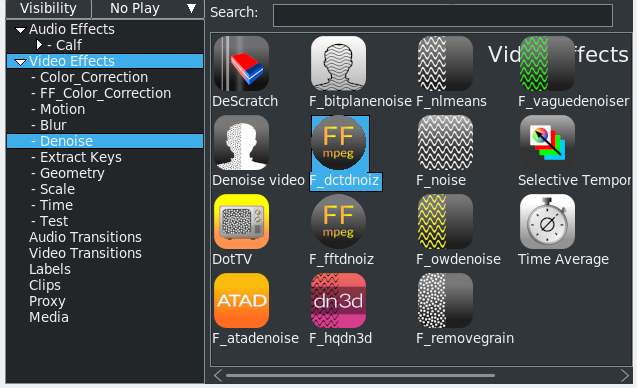
\includegraphics[width=0.8\linewidth]{expander.png}
    \caption{$\triangledown$,$\triangleright$ = expander; "-" = options}
    \label{fig:expander}
\end{figure}

\subsection{Speed-up of Ffmpeg plugin usage with OPTS files}%
\label{sub:speedup_ffmpeg_plugin_opts}

You can speed up some ffmpeg plugins that are quite time-consuming and use a lot of CPU\@. For a specific color-based example, \CGG{} uses 6 primary rendering color models. All of them have 3 components at full scale. Direct usage of a particular ffmpeg plugin from the ffmpeg command line might handle the planar at less than full scale chroma (yuv420), which means there is less data to manipulate. But when cinelerra loads a video it uses full scale color models. In other words:

\begin{itemize}[noitemsep]
    \item \CGG{} uses \textit{yuv444}
    \item ffmpeg uses \textit{yuv420}
\end{itemize}

if using an ffmpeg plugin that uses filters and many passes over the data, the amount of data is a big factor. If you load a file in \CGG{} with a

\texttt{same\_directory\_path\_and\_filename.opts}

file containing the following line, the full scale color modeling upgrade will not be performed until after any plugin, and then the render is faster:

\begin{lstlisting}[style=sh]
video_filter=xxxxxx=threads=8 # where xxxxxx is the desired filter
\end{lstlisting}

When the file loads, however, it will initially take longer because it is running through the video filter. The format \textit{rgb} in ffmpeg uses more cpu time. For comparison, ffmpeg line that might be used:

\begin{lstlisting}[style=sh]
ffmpeg -i /tmp/filename.mpeg -threads 15 -vf format=rgb24,xxxxxxs=threads=8 -acodec ac3 -vcodec libx265 - y /tmp/x.mp4
\end{lstlisting}

This converts the input to rgb before xxxxxx runs, and so it too is slower (because there is more color data). You would ordinarily avoid this conversion by omitting the \texttt{format=rgb24} parameter. An example ffmpeg plugin that could easily take advantage of an auxilliary opts file is \textit{nlmeans}.

\section{Audio Effects - Native}%
\label{sec:audio_effects_native}
\settocdepth{subsection}

\subsection{AudioScope}%
\label{sub:audioscope}

Effect rewritten and improved. Convert input audio to video output representing the audio power spectrum. Shows
% Yes
 %\todo{It's OK to use Subsection every plugin?}%
you the sound wave.

\subsection{Chorus}%
\label{sub:chorus}

It is a multitrack effect, where each track is a channel. For example if you have 4 voices per channel and 2 channels, you will have a total of 8 tracks.
It is an effect that modulates the signal, varies the pitch up and down (instead of modulating the phases as for example in the \textit{Flanger} plugin) and creates voices from the original signal and adds them to the Output. You then get a chorus effect, with multiple voices \textit{singing} the same song but with slightly different modulations. Voices not only modulate the original signal but also start with a certain delay. There are two components of delay, \textit{constant delay} and \textit{oscillating delay} (figure~\ref{fig:chorus}).

\begin{figure}[htpb]
	\centering
	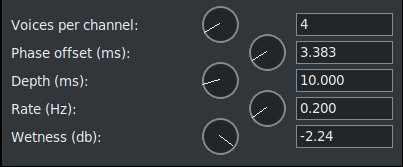
\includegraphics[width=0.5\linewidth]{chorus.png}
	\caption{GUI of configuration for Chorus plugin}
	\label{fig:chorus}
\end{figure}

\begin{description}
	\item[Voices per channel]: number of items we want to put in the effect. Using more than 4 voices creates sound artifacts that lose the feel of a human voice choir, but can still be used as an artificial sound effect.
	\item[Phase offset] (ms): is the constant delay, i.e.\ the amount of delay of the voices compared to the original signal.
	\item[Depth] (ms): is the oscillating delay, i.e.\ the delay in the oscillation of the various voices from the original signal.
	\item[Rate] (Hz): is the speed at which we apply the oscillating delay. In other words, the speed at which the oscillations occur.
	\item[Wetnwss] (db): Indicates how much of the original (dry) signal is taken into account compared to delayed voices.
\end{description}

\subsection{Compressor (Single Band)}%
\label{sub:compressor}

The audio compressor reduces the dynamic range of the audio, not the amount of data required to store the audio. In \CGG{} the compressor actually performs the function of an expander and compressor of the signal's dynamic range. A third and more sophisticated use serves to highlight the voice with respect to the sound background. It is a multitrack effect and can also be applied as a Shared Effect. (figure~\ref{fig:compressor}).

\begin{figure}[htpb]
    \centering
    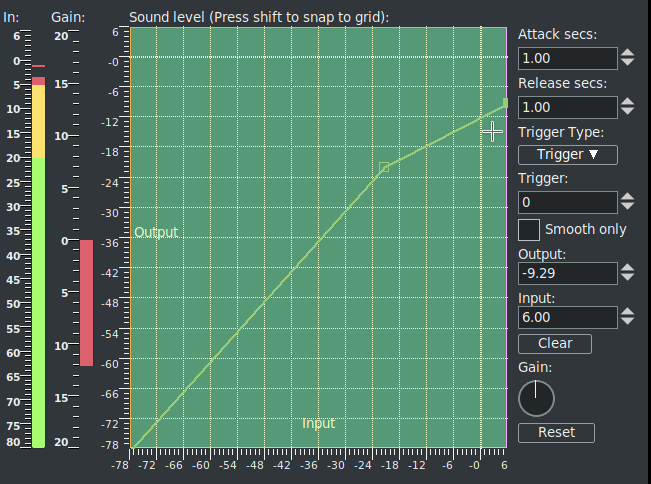
\includegraphics[width=0.7\linewidth]{compressor.png}
    \caption{GUI of configuration for Compressor plugin}
    \label{fig:compressor}
\end{figure}

The compressor works by calculating the maximum sound level within a certain time period of the current position. The maximum sound level is taken as the input sound level. For every input sound level there is an output sound level specified by the user.
The gain at the current position is adjusted so the maximum sound level in the time range is the user specified value.
The compressor has a graph which correlates every input sound level to an output level. The horizontal direction is the input sound level in dB. The vertical direction is the output sound level in dB. The user specifies output sound levels by creating points on the graph. Click in the graph to create a point. If two points exist, drag one point across another point to delete it. Moving the point horizontally is equivalent to the \textit{makeup gain} parameter. Note that it is impossible to create a vertical curve; points would be deleted.
Put a part of the curve in horizontal means clamping the signal to the same, unique value (as Limiter).
The most recent point selected has its values displayed in textboxes (Output and Input) for more precise adjustment.
To have the compressor reduce the dynamic range of the audio, make all the output values greater than the input values except 0\,dB. To make the compressor expand the dynamic range of the audio, make all the output values except 0\,dB less than the input values. The algorithm currently limits all sound levels above 0\,dB to 0\,dB, so to get an overloaded effect put a gain effect before the compressor to reduce all the levels and follow it with another gain effect to amplify all the levels back over 0\,dB.
The volume (in Db) of the input signal is shown in the \textit{In meter} on the left. Next to it is the \textit{Gain meter} which indicates the gain added (green) or subtracted (red) to the original signal according to our settings.

\begin{description}
    \item[Attack secs]: determines where in relation to the current position the maximum sound level is taken and how fast the \textit{gain} is adjusted to reach that peak. It is in seconds. If the reaction time is negative the compressor reads ahead of the current position to get the future peak. The gain is ramped to that peak over one reaction time. This allows it to hit the desired output level exactly when the input peak occurs at the current position. If the reaction time is positive the compressor scans only the current position for the gain and ramps gain over one reaction time to hit the desired output level. It hits the output level exactly one reaction time
    after detecting the input peak.
    \item[Release secs]: if the peak is higher than the current level, the compressor ramps the gain up to the peak value. Then if a future peak is less than the current peak it ramps the gain down. The time taken to ramp the gain down can be greater than the time taken to ramp the gain up. This ramping down time is the decay seconds.
    \item[Trigger type]: the compressor is a multi-channel effect. Several tracks can share one compressor. How the signal from many tracks is interpreted is determined by the \textit{trigger type}. The Trigger type uses the value supplied in the Trigger textbox as the number of the track to use as input for the compressor. This allows a track which is not even heard to determine the loudness of the other tracks. The maximum trigger takes the loudest track and uses it as the input for the compressor. The Total trigger type adds the signals from all the tracks and uses the total as the input for the compressor. This is the most natural sounding compression and is ideal when multiple tracks are averaged into single speakers.
    \item[Trigger]: This parameter is used in conjunction with trigger type as described previously. Normally only one track is scanned for the input peak. This track is specified by the Trigger. By sharing several tracks and playing with the trigger value, you can make a sine wave on one track follow the amplitude of a drum on another track, for example.
    \item[Smooth only]: for visualizing what the compressor is doing to the sound-level, this option causes it to replace the sound wave with just the current peak value. It makes it very easy to see how \textit{reaction secs} affects the detected peak values.
    \item[Gain]: moves the curve in the vertical direction only, to change the gain of the Output.
    \item[Clear] and \textbf{Reset}:  Reset the parameters to the default values (no compression).
\end{description}

\subsection{Compressor Multi (Multi Band)}%
\label{sub:compressor_multi}

Refer to Compressor (Single Band) for common theory and options.
The normal compressor acts over the entire frequency spectrum. The multi-band allows us to distinguish three frequency ranges (low, med and high) on which to intervene separately and in a more sophisticated way. In other plugins there are four bands instead of three, but we can make very precise adjustments so the three present are enough because they are not fixed. Finally the value of the three corrections are added together in the Output.

\begin{figure}[htpb]
	\centering
	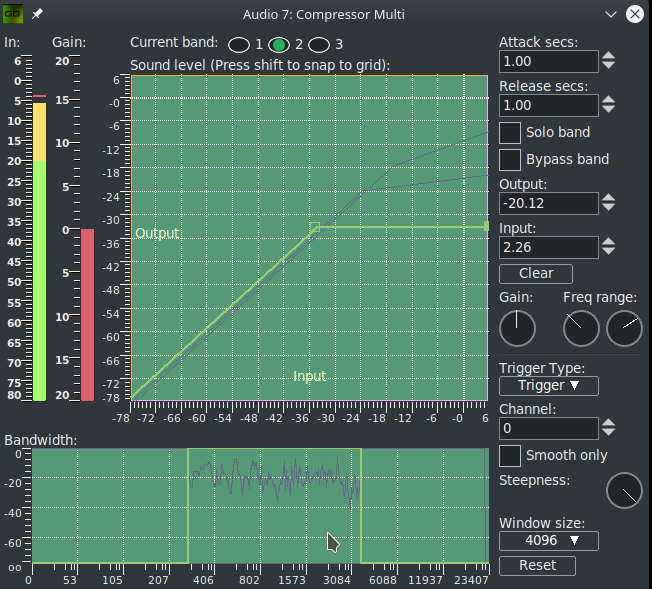
\includegraphics[width=0.7\linewidth]{compressorM.png}
	\caption{GUI of configuration for Compressor Multi plugin}
	\label{fig:compressorM}
\end{figure}

The three bands and their range (adjustable as desired) are shown in the frequency graph visible below (Bandwidth:).
As a first step you choose the band and adjust its range in the Bandwidth graph, then you go to adjust the compression in the top level graph. In this graph we can copy/paste the curve in the other bands via RMB; so we have a similar basis on which to make the adjustments.

In figure~\ref{fig:compressorM} we can see the three bands; the one currently active (\textit{Current band: 2}) presents the waveform of the sound signal. The interval goes roughly between 300\,Hz and 4000\,Hz, the edges are vertical because the \textit{stepness} is set to zero. So we have a clear separation between the bands, but by varying the slope we can have some overlapping of the bands for smoother effects. In the top level graph we can see the yellow curve of the active band, but we can also see in the violet the soft lines of the curves of band 1 and 2.

\begin{description}
	\item[Solo]: brings only the active band to the Output, silencing the others. So we can make more precise adjustments without listening to the whole effect.
	\item[Bypass band]: In contrast to Solo, it only brings the sound signals of the two inactive bands to the Output.
	\item[Freq range]: is used to set bandwidth limits. You act separately on the left and right edge.
	\item[Steepness]: varies the slope of the edges of the band range. Creates some overlap in the band boundaries.
	\item[Channel]: is the equivalent of the \textit{Trigger} option in Compressor (single band). Allows you to choose the channel or track to act on.
	\item[Window size]: Determines the number of samples used in the compression calculation. The more they are, the higher the quality of the result, but the more CPU usage.
\end{description}

\subsection{DC Offset}%
\label{sub:dc_offset}

Use this to remove \textit{DC Offset}, which is usually an undesirable characteristic of a recording normally caused by defective equipment. This effect works like a \textit{high pass filter} and has no controls. DC stands for \textit{Direct Current} which is the average amplitude of the waveform. It sounds best when it is absent, represented by zero, so that there is no imbalance in the audio.

\subsection{Delay Audio}%
\label{sub:delay_audio}

In the Delay Audio effect you can specify the number of seconds you want to delay the video track.

\subsection{DeNoise}%
\label{sub:denoise}

Reduce audio background noise. There is only 1 parameter which is used to regulate the level dial with a range of 0 to 1.

\subsection{DenoiseFFT}%
\label{sub:denoisefft}

Noise removal from audio using FFT editing. Set the Denoise Power dial in dB and choose the number of reference samples.

\subsection{Despike}%
\label{sub:despike}

Detect and eliminate out of range impulse values.

\begin{description}
    \item[Maximum level:] slider to set the maximum value in dB above which the frequency cutting takes place.
    \item[Maximum rate of change:] to adjust peak delete in dB.
\end{description}

\subsection{EQ Graphic}%
\label{sub:eq_graphic}

Graphic equalizer sets the output levels for specified frequency bands. This effect works by setting control points when you click the left mouse button and drag to the desired value. In the textboxes at the bottom can be seen the frequency of the active control point, the level of the signal to be set by entering the numerical value or by dragging the control point, and the number of samples to act on (figure~\ref{fig:equalizer}).

\begin{figure}[htpb]
    \centering
    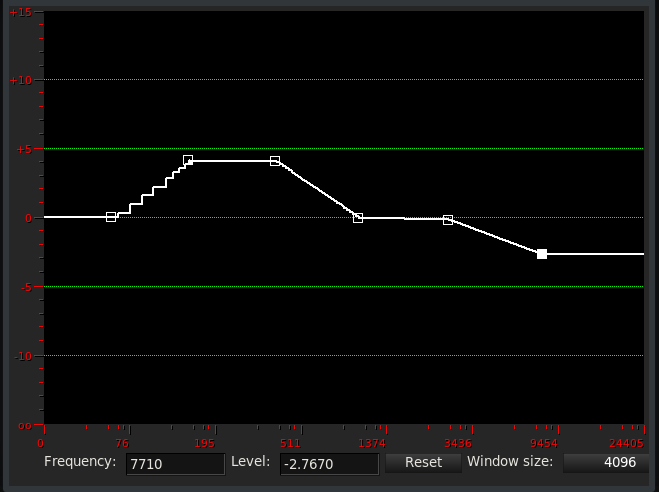
\includegraphics[width=0.8\linewidth]{equalizer.png}
    \caption{Graphic Equalizer audio plugin}
    \label{fig:equalizer}
\end{figure}

\subsection{EQ Parametric}%
\label{sub:eq_parametric}

Parametric equalizer shows and outputs levels for \textit{frequency}, \textit{quality}, \textit{level}, \textit{mode}, and \textit{wetness} (figure~\ref{fig:eq_param}).

\begin{figure}[htpb]
	\centering
	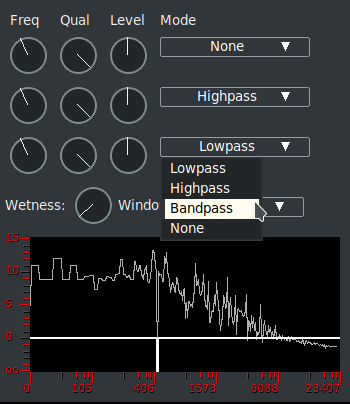
\includegraphics[width=0.4\linewidth]{eq_param.png}
	\caption{EQ Parametric audio plugin}
	\label{fig:eq_param}
\end{figure}

\subsection{Echo}%
\label{sub:echo}

Echo is reflection of sound. This plugin could be used to add echoing to video of your canyon hike (figure~\ref{fig:echo}).

\begin{figure}[htpb]
    \centering
    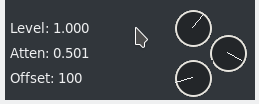
\includegraphics[width=0.4\linewidth]{echo.png}
    \caption{The 3 dials of Echo plugin}
    \label{fig:echo}
\end{figure}

\begin{description}
    \item[Level] represents the volume adjustment.
    \item[Atten] is attenuation which is a general term that refers to any reduction in the echo reflection. Sometimes called \textit{loss}, attenuation is a natural consequence of signal transmission over long distances.
    \item[Offset] is the lag in the attenuated echo signal. Offset means adding a DC level to a signal. It offsets the signal up or down in a DC sense without changing the size of the AC part of the signal. When you add an audio clip to the Timeline, the clip plays back from the beginning of the source audio file. The point in the audio file where the clip starts playing is called the offset. By default, a clip’s offset is zero, the beginning of the source audio file. You can change the offset so that the clip starts playing from a later point in the source audio file.
\end{description}

\subsection{EchoCancel}%
\label{sub:echocancel}

EchoCancel is the process of removing echos from audio in order to improve the quality. Echo cancel may be needed because an audio recording was done in a room that led to echo generation or there was some kind of unwanted feedback. There are many controls for the EchoCancel plugin which are defined here. However, the first thing you will see when you bring up the plugin, is the top portion that is black which will show a + in the middle when you mouse over it. Once you start playing audio, you will see the cepstrum spectral data inside the window. A cepstrum results from taking the inverse Fourier transform (IFT) of the logarithm of the estimated spectrum of a signal. It is used to identify the period of the echo in the audio. It is recommended to just set the \textit{Mode} to On but the below defined parameters can be utilized by professionals (figure~\ref{fig:echo-cancel}).

\begin{figure}[htpb]
    \centering
    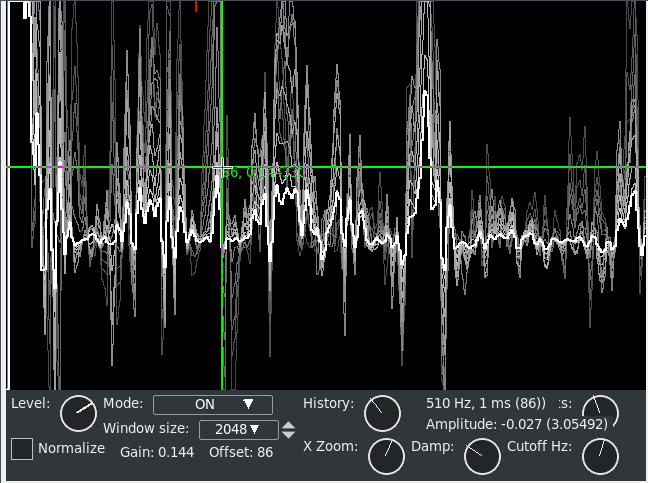
\includegraphics[width=0.8\linewidth]{echo-cancel.png}
    \caption{GUI for EchoCancel with crosshair and mode set to ON}
    \label{fig:echo-cancel}
\end{figure}

\begin{description}
    \item[Normalize:] audio normalization adds variable amounts of gain to an audio recording to bring the average or peak amplitude to a target level (the normal amount), on an ongoing buffer by buffer basis. This is to make the cepstrum graphical data appear between 0 and 1. Checkmark appears if ON.
    \item[Level:] scale factor used to draw the cepstrum output when normalize is not in effect.
    \item[History:] number of previous cepstrum outputs redrawn as fading graphical data.
    \item[X Zoom:] X axis scale factor to magnify low frequency cepstrum graphical output.
    \item[Damp:] echo envelope decay factor used to smooth the cepstrum/correlation data.
    \item[Peaks:] number of maximal envelope values used in the echo gain calculation.
    \item[Cutoff Hz:] low frequency cutoff value to prevent beat frequency (\textit{heterodyne}) echo canceling.
    \item[Mode:] \textit{MAN}, \textit{Off}, or \textit{On}. When Off is selected, the plugin is not active. When MAN is used, the only one peak is used for the echo gain envelope. It is set by pressing mouse button $1$ in the ceptstrum graphical output. The Gain and Offset are updated as the pointer drag operation resets the indicated gain and offset values. When On is selected, the echo gain envelope is automatically calculated by cepstrum and auto-correlation of the input audio in the last window size audio samples.
    \item[Windows size:] parameter can be set to \textit{Default}, $1024$, $2048$, \dots \textit{doubled values\dots} up to $262144$.
    \item[Amplitude:] the cepstrum value at the drag point during manual envelope selection.
    \item[Gain:] echo gain setting determined by manual selection.
    \item[Offset:] echo period setting determined by manual selection. The $Hz$ (frequency), $ms$ (millisecond duration), and sample offset (audio samples) as determined by manual selection.
\end{description}

\subsection{Flanger}%
\label{sub:flanger}

It's a single-track effect. If you apply it to multiple tracks each will work on its own track independently of the others.
It consists of making a copy of the original sound wave and then playing it over the original one with a certain delay. The resulting signal (Output) will then be the sum of the two waves and will have peaks where the two values add up and gaps where the two values compensate each other. The result is a more \textit{evanescent} and \textit{metallic} sound. Much, however, depends on the intensity of the effect.
The delay introduced consists of two distinct components: the \textit{constant delay} and the \textit{oscillating delay}. Their sum constitutes the total delay of the effect (figure~\ref{fig:flanger}).

\begin{figure}[htpb]
	\centering
	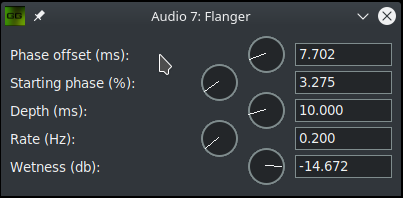
\includegraphics[width=0.6\linewidth]{flanger.png}
	\caption{GUI of configuration for Flanger plugin}
	\label{fig:flanger}
\end{figure}

\begin{description}
	\item[Phase Offset]: it is the constant delay. Once set, its value does not change (unless we change it, for example by use of keyframes) for the duration of the effect.
	\item[Starting phase] \%: is the point of oscillation where we start the oscillating delay; basically it is the attack value at which the effect starts the calculations. Not to be confused with the point on the timeline where we apply the effect. It only matches this for the 0\% value. The position on the timeline where we want to start the flanger at a given starting phase value can be chosen using keyframes.
	\item[Depth]: It is the oscillating delay. This value determines the amplitude variation of the delayed (wet) signal phase. This oscillation will be maintained for the entire duration of the effect unless we change it.
	\item[Rate]: is the speed at which we apply the oscillating delay. Low values indicate a lower oscillation frequency, a high value a rapid succession of oscillations.
	\item[Wetness]: indicates how much of the original (dry) signal is taken into account compared to the delayed (wet) signal.
\end{description}

\subsection{Freeverb}%
\label{sub:freeverb}

Adds effect of multiple decaying echoes to audio signals based on a specific algorithm. Common use of reverb is to simulate music played in a closed room.

\subsection{Gain}%
\label{sub:gain}

Add gain, input level, to increase/decrease loudness.

\subsection{Interpolate}%
\label{sub:interpolate}

Generate a smooth curve based on sound creating a certain softness. There are no controls.

\subsection{Invert Audio}%
\label{sub:invert_audio}

Reverses the numerical sign of the digital audio. There are no controls.

\subsection{Live Audio}%
\label{sub:live_audio}

The Live Audio effect reads audio directly from the sound card input. It replaces any audio on the track so it is normally applied to an empty track. To use Live Audio, highlight a horizontal region of an audio track or define In and Out points. Then drop the Live Audio effect into it. Create extra tracks and attach shared copies of the first Live Audio effect to the other tracks to have extra channels recorded. Live Audio uses the sound driver selected in \texttt{Settings $\rightarrow$ Preferences $\rightarrow$ Playback A $\rightarrow$ Audio Out for recording}, but unlike recording it uses the playback buffer size as the recording buffer size and it uses the project sample rate as the sampling rate. These settings are critical since some sound drivers can not record in the same sized buffer they play back in.

Live audio has been most reliable when ALSA is the recording driver and the playback fragment size is $2048$. Drop other effects after Live Audio to process sound card input in realtime. With live audio there is no read-ahead, so effects like compressor will either delay if they have read-ahead enabled or playback will under-run. A potential problem is that sometimes the recording clock on the sound card is slightly slower than the playback clock. The recording eventually falls behind and playback sounds choppy. Live Audio does not work in reverse.

\subsection{Loop Audio}%
\label{sub:loop_audio}

Loop some number of samples of audio over and over.

\subsection{Overlay}%
\label{sub:overlay}

Overlay has parameter settings of top or bottom for the track and add or multiply for the operation.

\subsection{Pitch Shift}%
\label{sub:pitch_shift}

Like the time stretching methods, there are three pitch shifting methods: \textit{Pitch shift}, \textit{Resample}, and \textit{Asset info} dialog. Pitch shift is a realtime effect which can be dragged and dropped onto recordable audio tracks. Pitch shift uses a fast Fourier transform (FFT) to try to change the pitch without changing the duration, but this introduces windowing artifacts. Because the windowing artifacts are less obtrusive in audio which is obviously pitch shifted, Pitch Shift is mainly useful for extreme pitch changes. For mild pitch changes, use Resample instead. Another way to change pitch slightly is to go to the Resources window, highlight the media folder, right click on an audio file, click on \textit{Info}, then adjust the sample rate in the Info dialog to adjust the pitch. This method also requires left clicking on the right boundary of the audio tracks and dragging left or right to correspond to the length changes.

\subsection{Remove Gaps}%
\label{sub:remove_gaps}

Remove silent gap (below $DB$ threshold) which persist for more than the time limit.

\subsection{ResampleRT}%
\label{sub:resamplert}

Allows you to convert an audio file from one sample rate to another. This effect works similarly to ReframeRT in videos.

\begin{center}
    \begin{tabular}{l l}
        \toprule
        Input / output > 1 &	fast rate \\
        Input / output < 1 &	slow rate \\
        \bottomrule
    \end{tabular}
\end{center}

\subsection{Reverb}%
\label{sub:reverb}

Reverb uses reflections of sound to add depth and fullness; the sound will seem to come from a space that can go from a small bare room to large natural valleys, cathedrals, etc. The reverb is made up of a group of echoes that occur at the same time making it feel like a single effect.
Basically simulates creation of a large number of reflections, like lots of walls, which build up and then decay. You can use the reverb plugin to mix tracks together to simulate ambiance because it is a multitrack effect.
The configuration window (figure~\ref{fig:reverb}) shows a graph of the full band pass filter frequencies.

\begin{figure}[htpb]
	\centering
	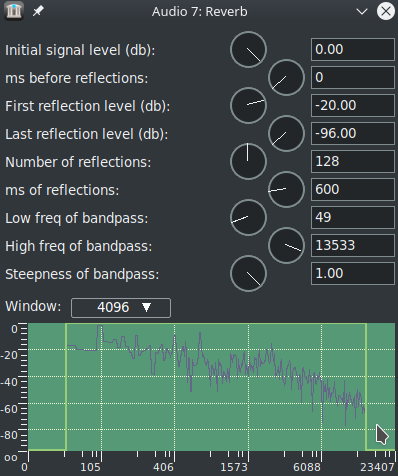
\includegraphics[width=0.6\linewidth]{reverb.png}
	\caption{GUI of configuration for Reverb plugin}
	\label{fig:reverb}
\end{figure}

\begin{description}
	\item[Initial signal level](db): Allows you to set the level of the reflected signal. At 0 you start from its maximum level. Decreasing the signal volume will give more presence to the original signal.
	\item[ms before reflections]: indicates when to start the reflected sounds in relation to the original sound  (delay).
	\item[First reflection level] (db): the sound level of the reflection that starts first.
	\item[Last reflection leve] (db): the level of the last reflection. It is weaker than the first.
	\item[numbers of refelctions]: the number of reflections can be set as desired as long as there is sufficient CPU to handle it. With a few reflections you get closer to the Chorus effect. You can start from values of 100 - 150, up to a maximum of 255.
	\item[ms of refelction]: Sets the action time of the effect. With high values, the sound is more clear and sharp
	\item[Low freq of bandpass] and \textbf{High freq of bandpass}: allow you to set the frequency limits (range) on which the effect acts.
	\item[Steepness of bandpass]: allows you to adjust the slope of the frequency range limits imposed by the previous items. With the value 1.00 we have a vertical edge that clearly separates the range of frequencies on which to act from the remaining ones (as you can see in figure~\ref{fig:reverb}). By sloping the edge we have a certain overlap and a smoother effect.
	\item[Window]: determines the number of frequency samples taken into account by the effect for its calculations. The higher the number, the smoother the effect; but more CPU is used.
\end{description}

\subsection{Reverse Audio}%
\label{sub:reverse_audio}

Apply reverse audio to an audio track and play it backwards. The sound plays forward. Be aware when reversing audio that the waveform on the timeline does not reflect the actual reversed output.

\subsection{SoundLevel}%
\label{sub:soundlevel}

Effect rewritten and improved to handle fragments. Displays the Max/RMS sound level in decibels.

\subsection{Spectrogram}%
\label{sub:Spectrogram}

Effect rewritten and improved. Visual representation of the sound levels at specified frequencies as they vary with time.

\subsection{Synthesizer}%
\label{sub:Synthesizer}

Generate synthesizer sounds; to set key data, turn on Generate keyframes while tweaking (figure~\ref{fig:synthesizer}).

\begin{figure}[htpb]
    \centering
    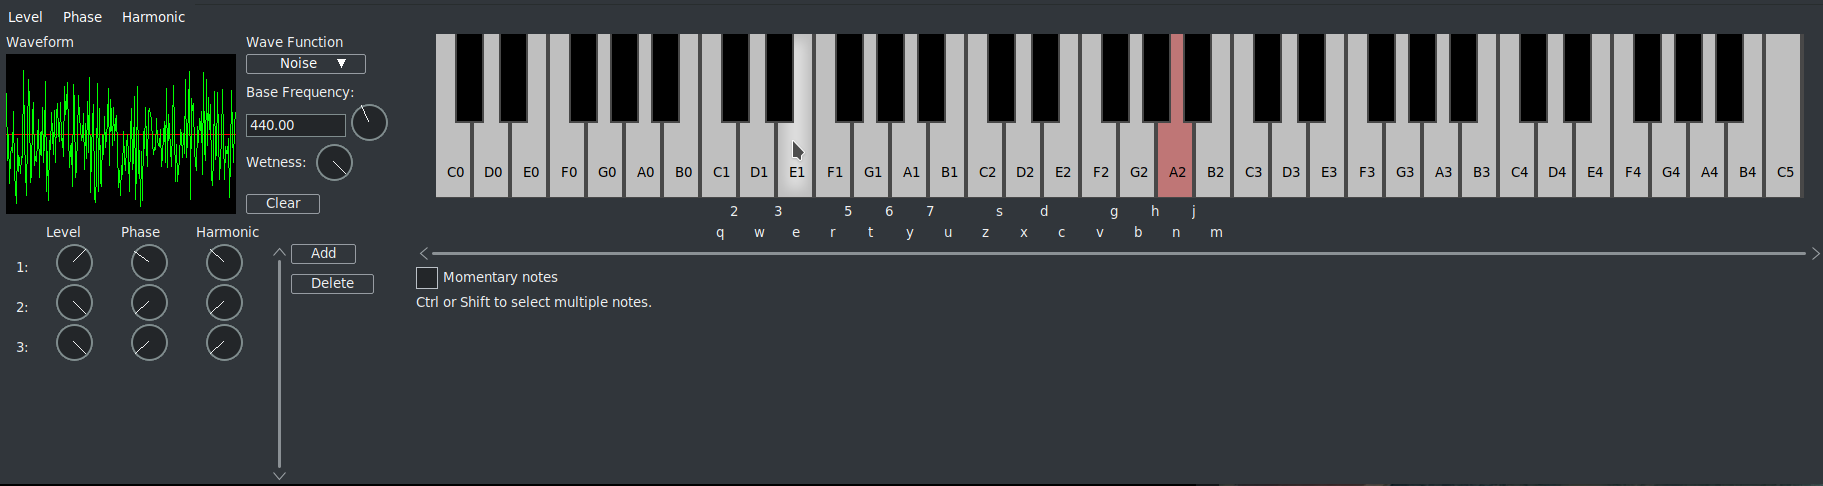
\includegraphics[width=1.0\linewidth]{synthesizer.png}
    \caption{GUI for Synthesizer}
    \label{fig:synthesizer}
\end{figure}

\subsection{Time Stretch RT}%
\label{sub:time_stretch_rt}

Change the speed of an audio signal without affecting its pitch.

\subsection{Tremolo}%
\label{sub:tremolo}

It serves to give various vibes and vitality to the sound by modulating the amplitude of the sound signal and the delay (figure~\ref{fig:tremolo}).

NOTE: There is often confusion between Tremolo and Vibrato, but the vibrato is the periodic variation of the height of a note (frequency) while the tremolo is the periodic variation of the height (amplitude) of the sound wave.

\begin{figure}[htpb]
	\centering
	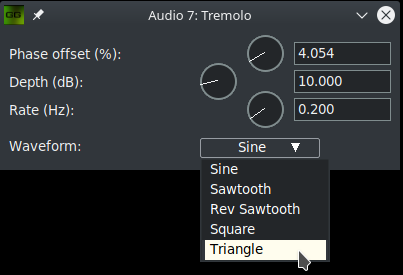
\includegraphics[width=0.5\linewidth]{tremolo.png}
	\caption{GUI of configuration for Tremolo plugin}
	\label{fig:tremolo}
\end{figure}

\begin{description}
	\item[Phase offset] (\%): is where the oscillation effect begins. At 0\% we are at maximum volume; to lower the volume, increase the percentage.
	\item[Depth] (dB): is the oscillation damping value. You can only decrease the level, you cannot increase it.
	\item[Rate] (Hz): is the speed at which the oscillations are repeated.
	\item[Waveform]: you can choose waveform algorithms to use in effect calculations.
Currently available waveforms are: \textit{Sine}; \textit{Sawtooth}; \textit{Rev Sawtooth}; \textit{Square} and \textit{Triangle}.
\end{description}

\section{Audio Ladspa Effects}%
\label{sec:audio_ladspa_effects}
\settocdepth{section}

Ladspa effects are supported in realtime and rendered mode for audio. These audio effects are supported since \CGG{} implements the LADSPA interface as accurately as possible. Besides the supplied LADSPA effects\protect\footnote{credit Steve Harris}, additional LADSPA effects can be enabled by setting the \texttt{LADSPA\_PATH} environment variable to the location of your LADSPA plugins:

\begin{lstlisting}[style=sh]
export LADSPA_PATH=/usr/lib/ladspa
\end{lstlisting}

\section[Audio LV2 / Calf Plugins]{Audio LV2 / Calf Plugins\protect\footnote{Optional Feature - OS dependent}}%
\label{sec:audio_lv2_calf_plugins}

LV2 is an open standard for audio plugins using a simple interface with extensions which add functionality to support audio software. These plugins were written by external developers and provide additional audio effects to \CGG{} audio without having to change \CGG{} every time. Because the LV2 plugins are separate from \CGG{} Infinity, if one fails or does not perform as expected, \CGG{} should stay running and you will have to contact the programmers responsible for that plugin for a fix.

Typically, a user OS has specialized package groups installed. It is difficult to create one build of \CGG{} to accommodate all potential LV2 plugins. Specifically for the \textit{Calf-Studio LV2 plugins}, you should install the \textit{Calf Plugins} package. The user’s computer must have \textit{gtk-2-runtime} installed, which seems to be automatically done already for most distros. For users doing their own builds, you can build \CGG{} without LV2 support by including \texttt{-{}-without-lv2} in the configure step. The default build is \texttt{-{}-with-lv2=yes} and requires that \textit{GTK-2-devel} must be installed or the build will fail and notify you.

LV2 plugins have their own category in the \textit{Audio Plugins Visibility} as lv2. There is a simple text interface which is available via the usual \textit{Show controls} button when the plugin is attached to the audio track. This window has a Reset button to get back to the default settings. To change a value of one of the parameters, highlight that parameter and type in the new value in the topmost text box and then hit Apply to take effect -- the reason for requiring hitting apply is so that the audio is not moving all over the place while you are still typing a value. More easily, you can just move the \textit{pot dial} or the \textit{slider} bar which take effect automatically.

\CGG{}’s buffer size setting may cause a delay in activation of the changes you make taking effect, so you can lessen the time by using a small buffer. Notice that $1024$ samples at $48000$ samples per sec is only $\frac{1}{50}^{th}$ a second. This is not a lot of time to shuffle a bunch of stuff. Short buffers produce low latency, but no time for complex programs or lots of stacked effects. Bigger buffers allow for more complex setups.

To set the buffer size:

\texttt{Settings $\rightarrow$ Preferences $\rightarrow$ tab Playback A $\rightarrow$ section Audio Out $\rightarrow$ variable Playback buffer samples}

However, be forewarned that due to variability in the lv2 plugin programming code, some of the plugins only work with the minimum buffer size of $1024$. In these cases, what you will see is the main track canvas cursor just bounces back and forth over a very small area in the timeline. This does not crash \CGG{} but you will have to remove the plugin to continue working.
You can specify a certain set of LV2 plugins to use by setting \texttt{LV2\_PATH} as shown below before starting \CGG{} -- include a colon ($:$) separator for multiple paths. The default path for most operating systems is \texttt{/usr/lib64/lv2}. To list the system installed lv2 plugins key in: \texttt{lv2ls}.

\begin{lstlisting}[numbers=none]
export LV2_PATH=/tmp/j/balance.lv2/usr/local/lib/lv2/:/usr/local/lv2
\end{lstlisting}

If there is no default \texttt{LV2\_PATH} set automatically, the value will be \texttt{\$CIN\_DAT/\\lv2}, which is a placeholder only so that no lv2 plugins will be loaded. When there is no system \texttt{LV2\_PATH} set it is important to note, that if you do want lv2 plugins loaded, you must set the correct path in:

\texttt{Settings $\rightarrow$ Preferences $\rightarrow$ Interface tab $\rightarrow$ Default LV2 $\rightarrow$ direc\-tory
    path name}

When you change this field, cin will automatically restart and load the newly specified lv2 plugins. If when switching \texttt{LV2\_PATH} or if the lv2 audio plugins are not displayed/usable in the Resources window, you can execute a reload via:

\texttt{Settings $\rightarrow$  Preferences $\rightarrow$ Interface tab $\rightarrow$ Reload plugin in\-dex}
or else before you bring up \CGG{}, delete \texttt{\$HOME/.bcast5/\CGG{}\_\\plugins} so that the plugins get properly reloaded.

There are some lv2 plugins that display a \textit{glitzy} UI (User Interface); for example the \textit{Calf plugins}. For these LV2 plugins, if you want that to automatically come up without having to click on the UI button on the simplified UI interface, there is a flag to enable that. It is at:

\texttt{Settings $\rightarrow$ Preferences $\rightarrow$ Operations} tab

then check the \textit{Auto start lv2 gui} Flag

Below is a screencast showing the auto start gui flag and the \texttt{LV2\_PATH} default directory path on the bottom line. Note the highlighted \textit{Reload plugin index} which will be executed if OKed (figure~\ref{fig:reload}).

\begin{figure}[htpb]
    \centering
    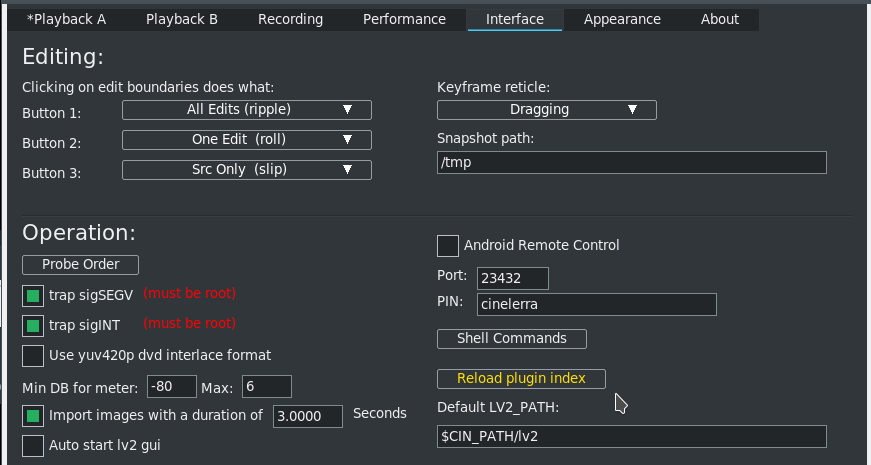
\includegraphics[width=1.0\linewidth]{reload.png}
    \caption{Reload plugin index in yellow and Auto start lv2 gui unchecked}
    \label{fig:reload}
\end{figure}

There is also a blacklist that prevents known problematic-for-\CGG{} lv2 plugins from loading to avoid crashes. If others are found to have problems, once informed about them, they will be added to this blacklist. In order to determine which lv2 plugin causes a SEGV on \CGG{} startup, you can start from a terminal window and you will see each plugin that is being loaded and the last one shown before the crash is a bad plugin. However, many of the plugins causing a crash are due to not having been compiled on your current system with the current compiler so may actually work correctly on other user systems and so will not be added to the \CGG{}-wide blacklist. You can either recompile the problematic plugin, or modify your own blacklist which you will have to maintain and save so as not to be written over when loading a new build.

Note the UI button in the upper right hand corner above the Reset button (figure~\ref{fig:calf}). If you click this button, a glitzy interface window comes up (if available) for changing variable values. It is possible that a bug in the LV2 plugin causes the glitzy window to appear as blank and then die, but in that case the original simple text window might still work -- in either case, if the timeline movement hangs, just detach the plugin to continue your current session. There is an environment variable that you can set,  \texttt{BC\_TRAP\_LV2\_SEGV}, to get a dump of the failure which may be helpful for debugging.

\begin{figure}[htpb]
    \centering
    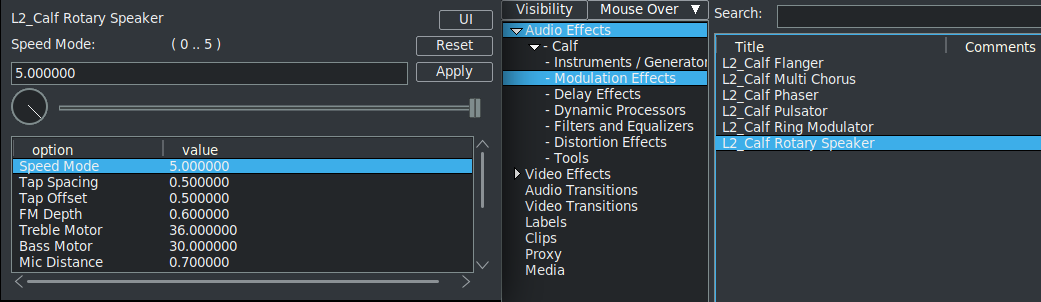
\includegraphics[width=1.0\linewidth]{calf.png}
    \caption{Screencast of simple text interface in the middle of the screen for a Calf LV2 plugin}
    \label{fig:calf}
\end{figure}

When the glitzy ui is up, the simple text window remains up also since it is the \CGG{} side and keeps track of the value changes so they remain in effect for further usage of the plugin. Changes to one or the other will occur in both with the exception of certain features in the glitzy window which are not communicated correctly back to \CGG{}; for example a reset button -- the simple interface Reset button must be used instead. To change values in the glitzy window you use the mouse and move up or down unlike a knob that turns! (Figure~\ref{fig:calf02})

In order to test a particular plugin without bringing up \CGG{}, especially for ones that do not operate, it is possible to manually display an lv2ui gui with: \\
\texttt{/cin-path/lv2ui <lv2-uri>} \\
For example:

\begin{lstlisting}[style=sh]
/tmp/cinelerra-5.1/bin/lv2ui http://calf.sourceforge.net/plugins/Flanger
\end{lstlisting}

\begin{figure}[htpb]
    \centering
    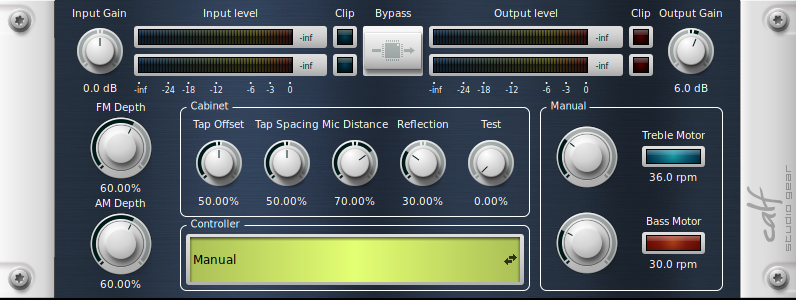
\includegraphics[width=0.8\linewidth]{calf02.png}
    \caption{Screencast with a Calf plugin glitzy window that appears when clicking the simple interface UI button.}
    \label{fig:calf02}
\end{figure}

\section[Video Effects --- Native]{Video Effects -- Native}%
\label{sec:video_effects_native}
\settocdepth{subsection}

\subsection{1080 to 480}%
\label{sub:1080_to_480}

Most TV broadcasts are received with a $1920\times1080$ resolution but originate from a $720\times480$ source at the studio. It is a waste of space to compress the entire $1920\times1080$ if the only resolvable details are $720\times480$. Unfortunately resizing $1920\times1080$ video to $720\times480$ is not as simple as shrinking it.

At the TV station the original $720\times480$ footage was first converted to fields of $720\times240$. Each field was then scaled up to $1920\times540$. The two $1920\times540$ fields were finally combined with interlacing to form the $1920\times1080$ image. This technique allows a consumer TV to display the re-sampled image without extra circuitry to handle $720\times480$ interlacing in a $1920\times1080$ image.

If you merely deinterlace the $1920\times1080$ images, you would end up with resolution of $720\times240$. The \textit{1080 to 480} effect properly extracts two $1920\times540$ size fields from the image, resizes them separately, and combines them again to restore a $1920\times480$ interlaced image. The scale effect must then be applied to reduce the horizontal size to $960$ or $720$ depending on the original aspect ratio.

The tracks to which \textit{1080 to 480} is applied need to be at $1920\times1080$ resolution. The project settings in \texttt{settings $\rightarrow$ format} should be at least $720\times480$ resolution. The effect does not know if the first row in the $1920\times1080$ image belongs to the first row of the $720\times480$ original. You have to specify what the first row is in the effect configuration. The output of this effect is a small image in the middle of the original $1920\times1080$ frame. Use the projector to center the output image in the playback.

Finally, once you have $720\times480$ interlaced video you can either apply \textit{Frames to Fields} or \textit{Inverse Telecine} to further recover original progressive frames.

\subsection{1080 to 540}%
\label{sub:1080_to_540}

Extracts two $1920\times540$ fields from $1920\times1080$ image, resizes them separately, and combines them to $1920\times540$ interlaced image.

\subsection{Aging TV}%
\label{sub:aging_tv}

This effect is the one to use if you want to achieve an old movie or TV show look. It will put moving lines up and down the movie as well as putting snow on the video. Use it along with \textit{Brightness/Contrast} and \textit{Color Balance} to make your movie look like a really old black and white movie. This came from \url{https://effectv.com}.

\subsection{Alpha}%
\label{sub:alpha}

Allows you to apply an alpha value (transparency) to one or more tracks or one or more edits. Being also keyframable, it allows an excellent variety and possibility of use in the most disparate occasions.

\subsection{Auto Scale}%
\label{sub:auto_scale}

Automatically scale to a specified size.

\subsection{Blue Banana}%
\label{sub:blue_banana}

Blue Banana\protect\footnote{credit to Monty Montgomery programmer} is an \textit{HSL Qualifier} (HSL= hue, saturation, lightness), one of the basic tools of any grading software that are based on circumscribing a zone of the frame by extracting a chromatic key and producing a \textit{matte} in the alpha channel (Secondary Color Correction). Blue Banana differs not by creating a real matte, but by creating a \textit{selection mask} exclusively for use within the plugin. The BlueBanana plugin has a couple of useful purposes. It can be used for color transformation or remapping -- by isolating a specific color and then performing color change/correction on only that color (or color ranges). Another useful purpose is for chroma-key filtering, using multiple BlueBanana plugins on the same track. Also, it can be used in conjunction with the mask operation of the Compositor. Usage of BlueBanana may seem complicated at first, but it is necessarily so in order to get enough control to produce the desired effect simply and quickly. Just changing a single color is actually quite easy. BlueBanana is keyframable (figure~\ref{fig:bluebanana}).

The basic strategy for BlueBanana is to:

\begin{itemize}
    \item Select a specific target color.
    \item Create a selection region by expanding color ranges around that color.
    \item Optionally reduce or expand the alpha plane as a regional selection mask.
    \item Optionally apply a color remapping or transformation to the selection.
    \item Optionally reset the output alpha to opaque, or pass the alpha to another BlueBanana plugin.
\end{itemize}

\begin{figure}[htpb]
    \centering
    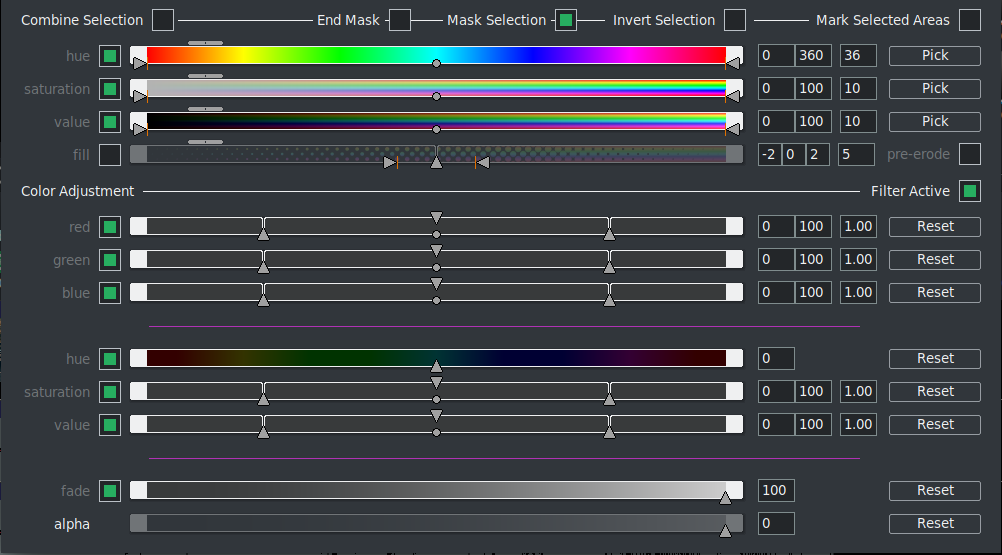
\includegraphics[width=1.0\linewidth]{bluebanana.png}
    \caption{Screencast showing the BlueBanana plugin control}
    \label{fig:bluebanana}
\end{figure}

\subsubsection*{Just a Warning Note:}
\label{ssub:warning_note}
BlueBanana may use a lot of CPU and Memory because it is doing a lot of work. If you turn off the plugin on the plugin bar below the video track in the main track canvas it will stop using cpu when not in use. Or once you uncheck \textit{Mark Selected Area}, it will no longer be using the cpu to mark the selected color area in realtime while drawing the diagonal animated pattern in the compositor window.

\subsubsection{Example Usage\protect\footnote{from original message by Rebecca}}
\label{sssec:example_usage}

If you just want to try this, follow these steps.

\begin{description}
    \item[First ---] Choose your color.
    \begin{enumerate}
        \item Load your video, add the BlueBanana plugin to the track, bring up its control window, and uncheck any checked boxes (mostly just to avoid unexpected results).
        \item In the Compositor window, choose the eyedropper color picker tool on the left-hand side and click on the area of the image that shows the color you want to change/correct.
        \item In the BlueBanana plugin window, to the right of hue, click Pick. And if you want to modify saturation and value, also click on the Pick button for them. To see what it does, Pick them also.
        \item Next, check the Mark Selected Areas box at the top right of the BlueBanana plugin window to see the selected color-matching areas which will become marked in a diagonally striped pattern.
        \item You can now manually modify your selection in the Color Selection area in the obvious ways for hue, saturation, value and fill. The arrows to each side of the small circle widen the selected area. Move the dot and you move the range. The slider on top of the horizontal color strip shifts like the amount of the strip is dedicated to that part of the color spectrum. Fill will fill more area or less area in your selected region.
    \end{enumerate}
    \item[Second ---] Adjust your color choice.
    \begin{enumerate}
        \item There are color strips under color Adjustment which will show color changes as you modify values.
        \item Uncheck Mark Selected Areas and check the Filter Active box to the right of Color Adjustment.
        \item As needed, you can individually check and uncheck all the various parameters using the boxes to the left of each line. Again, these are intuitive and broadly similar to the above. The arrows at the bottom widen the range, the circle at the bottom moves the range, and the top slider, which is an arrow this time, affects distribution. It provides a little histogram effect to give you an idea of what you're changing. The fade adjusts the level of color blending. The alpha is basically the opacity of your changes.
    \end{enumerate}
\end{description}

Definition of Wording/Checkboxes/Buttons/Operators are being described next. Some of the commentary was adopted from information provided by \textit{Monty Montgomery} and from questions and answers from email by \textit{Igor Ubuntu}, who did extensive testing.

\subsubsection*{Operational characteristics for the \textbf{color-related adjusters}:}
\label{ssub:operational_characteristic_color}

\begin{description}
        \item[left arrow slider] operates the range minimum; the numerical value shows in the left-most textbox.
        \item[right arrow slider] operates the range maximum; resulting numerical value is in the middle textbox.
        \item[middle circle slider below] can move the current range up or down and the numerical results will show in the left and middle textbox. Move the dot and you move the range.
        \item[top pad slider] operates the edge slopes (selection attack/decay) and the value will be displayed in the
        rightmost textbox. Sharp edges are represented by 0; 100 represents smooth edges.
        \item[top arrow] affects the distribution skew.
\end{description}

\subsubsection*{Operational characteristics for \textbf{Fill}:}
\label{ssub:operational_characteristic_fill}

\begin{description}
        \item[left arrow slider] operates mask erosion filling. First textbox value.
        \item[center up arrow slider] operates the fill skew midpoint. Second textbox value.
        \item[right arrow slider] operates mask expansion filling. Third textbox value.
        \item[top pad slider] operates the edge slopes. Right textbox value.
\end{description}

The textboxes are available so that you can directly type in numbers from the \textit{color wheel}. This could be helpful if duplicating previous work as it would be an instantaneous exact numerical match without having to continuously fine-tune the movement of a slider.

There are two panes separated by long horizontal lines (through the middle of the screen) in the control window of the BlueBanana plugin, clearly visible in the previous screencast. The top pane is first used to create/modify a selection, and the bottom pane is used to operate a change.

\subsubsection*{Pane 1}
\label{ssub:pane1}

This section is used to select the target color domain. First, a short explanation about alpha. The alpha channel used in BlueBanana is not transparency (\textit{matte}); it is used as the \textit{Selection mask}. Alpha plane is the alpha channel of the current image. So that:

RGBA = red/green/blue color planes, alpha data plane.
YUVA = luma/Cb/Cr color values, alpha data plane.

The alpha data normally is input to the blending operations in the patchbay overlay mode. The alpha data usually creates the appearance of stacking order, and determines which color planes are visible in the rendered result. When BlueBanana is used, the meaning of the alpha data is changed to the selection. It is useful to think of the alpha data as more solid when it is transparency in blending, and more selected when it is used in BlueBanana. In both cases, the greater the alpha value, the more the effect is expressed.

Usually, alpha is normalized to a range from $0$ to $1$, zero = no effect, $1$ = total effect, $0.5$ = partial effect. In both cases, alpha is what math people call an auxiliary variable. It is needed, but is not part of the answer. In this case, the answer is the visible rendered result. Alpha is like meta-data.

Let us now examine the instruments in \textbf{pane 1}:

\begin{description}
    \item[Combine Selection] The selection is the intersection or union of two pixel masks. Mathematically, $A$ and $B$ are normalized, (scaled to between $0$ and $1$) and used as selection mask weights.

    $Intersection (\cap) = A\times B$

    $Union (\cup)= A+B-A\times B$

    where $A$ is the input alpha plane as a mask, $1$=selected, $0.4$=partially selected, and $0$=not selected; $B$ is the color selection of trims and feathers made by varying the sliders.

    The result is a new alpha plane, which will be output (if \textit{End Mask} is not set). The $0\dots1$ selection values are used to weight the color transformation filters if/when they are active and operate a change. The color adjustment filters available in Pane \#$2$ can change red, green, blue, and remap hue, saturation, value in the pane. There is also \textit{fade} which applies to the color channels and \textit{alpha} which applies to the resulting alpha plane.

    The basic plan is to either:

    - reduce a selection area by intersection (Combine selection off) $A \times B$

    - increase a selection area by union (Combine selection on) $A+B-A\times B$
    \item[Mask Selection] applies the current mask to the selection, such that the mask clips/expands the selection. When mask selection is enabled, the result of the and/or will be stored to the alpha result, but when mask selection is unchecked the mask is ignored and the selection is not modified. The selection is used to weight the effect of the filtering, or to control the output alpha.
    \item[End mask] only visible when \textit{Mask Selection} is checked. End Mask causes the entire alpha plane to
    be set to $1$. The image becomes opaque. This is usually only set in the last plugin of a stack (the stack may be just one plugin doing only color modification). In the event that a color selection mask is used with multiple, layered BlueBanana filters on the same track, the grouped BlueBanana filters may share a single mask by all enabling Mask Selection, but with only the last BlueBanana enabling End Mask. This usage pattern gives the End Mask control its name.
    \begin{description}
        \item[End Mask as used in Color Transformation/Remapping:] In many use cases \\
        where you are just remapping color, you are still interested in seeing all of the picture. If this is the case, then checking End Mask on the last BlueBanana plugin will show you the entire picture. The alpha plane may be in use as a selection mask, but it may not be wanted as part of the result.
        \item[End Mask as used in Chroma-key Filtering:] In cases where the selection is for a chroma-key, you are interested in the alpha channel for blending, like \textit{Normal} or \textit{SrcOver}. So for this usage of the BlueBanana, don't check the End Mask.
    \end{description}
    \item[Invert Selection] reverse target color domain, which is 1 minus selection.
    \item[Mark Selected Areas] when this box is checked, the chosen colors are presented in an animated
    diagonally striped pattern.
    \item[Hue] select a hue domain; click on the Pick button to select or check the box to the left of hue or uncheck to ignore.
    \item[Saturation] select a saturation domain; click on the Pick button to select or check the box to the left.
    \item[Value] select a value domain; click on the Pick button to select or check the box to the left.
    \item[Fill] will fill more area or less area of your selected region. This describes how it works. Fill control is an automated way of doing grow and shrink on the selected area, to fill in small holes, or get rid of scattered speckles. If none of the Hue, Saturation, or Value sliders are active -- meaning that the whole frame is selected -- the Fill slider will have no effect even when enabled. The word fill will appear ghosted to indicate this.

    The three lower handles in the fill slider correspond to \textit{Shrink} (the left hand slider), \textit{Final} (the middle slider), and \textit{Grow} (the right hand slider). These are used in combination to alter the selection by first growing it by the amount specified by the right hand Grow slider, shrinking it to the amount specified by the left hand Shrink slider, and then growing it again to the final size specified by the middle Final slider. The top slider then feathers the resulting selection.
    Growing the selection and then shrinking it has the effect of filling small holes in the selected area. Similarly, shrinking and then growing tends to remove small flecks of unwanted selection. The Final slider specifies the overall desired shrinkage or growth of the selection when finished. To specify a pure Grow or Shrink operation, set the Final slider and the Grow/Shrink slider to the same value and leave the other slider at zero.
    \item[Pre-erode] this control reverses the order of operation to Shrink, then Grow, then Final. The change is subtle on most images, but overall removes more small features because it first removes flecks before filling in holes.
\end{description}

\subsubsection*{Pane 2}
\label{ssub:pane2}

This section is used to modify the color of your selection. Descriptive commentary for this pane.

\begin{description}
    \item[Filter Active] checkbox to indicate that the modifications will be shown.
    \item[Color Adjustment ] For Color Adjustment, RGB can be used as color weights while the HSV can transform color.
    For the following items there are three sections on the slider. The \textit{center} section represents the nominal $0\%-100\%$ range; the \textit{left} section represents negative values, and the \textit{right} section represents values greater than $100\%$. Values can be out-of-range within BlueBanana without clipping, but they will clip once they leave the plugin.
    \item[RGB] affect the color channels individually.
    \begin{description}
        \item[Red] modification color; click the Reset button to revert to default. Values are reflected in numerical textboxes on the right-hand side.
        \item[Green] modification color; click the Reset button to revert to default. Values are reflected in numerical textboxes on the right-hand side.
        \item[Blue] modification color; click the Reset button to revert to default. Values are reflected in numerical textboxes on the right-hand side.
    \end{description}
    \item[HSV] reorient the color spectrum, and affect all of the color channels simultaneously.
    \begin{description}
        \item[Hue] a single numerical value will appear in the right-side box. Click the Reset button for default.
        \item[Saturation] for modifying the saturation; click the Reset button to revert to default. Values are reflected in numerical textboxes on the right-hand side.
        \item[Value] for modifying the value; click the Reset button to revert to default. Result is reflected in the numerical textboxes on the right-hand side.
    \end{description}
    \item[Fade] controls the entire color re-mapping, and does nothing if no color adjustment is active.
    \item[Alpha] controls the output alpha (this is not available when End Mask is set); click the Reset button to revert to default. Result is reflected in the numerical textboxes on the right-hand side.
\end{description}

Let's see two examples of HowTo:


\subsubsection*{BlueBanana Use Case \#1: (Color Transform/Remapping)}
\label{ssub:bb_use_case_1}

\begin{itemize}
        \item Load a video track, and add the BlueBanana plugin to your video. The alpha channel is usually all opaque. This serves as an initial full screen selection mask.
        \item Open the controls, and start with all boxes unchecked. Now reduce the selection using the top pane in intersection mode (that is \textit{Combine Selection} is unchecked) to begin the effect.
        \item Use the \textit{eyedropper} on the compositor window to choose a particular color.
        \item Click on the 3 plugin Pick boxes on the right side of each line of HSV to get the color selection.
        \item Check \textit{Mark Selected Area}. The affected zones will be identified on the composer.
        \item Adjust the selection using the HSV and Fill sliders of the top pane. The selection mark will be updated as you operate the controls. The composer mask striping will be strongest as the mask is nearer full selection.
        \item Now uncheck \textit{Mask selected area} \& check \textit{Filter Active} to begin Color Adjustment.
        \item Enable any needed colorspace modifiers, RGB / HSV sliders, and setup the color changes by moving the sliders. The current output may be the desired output.
        \item Enable \textit{Mask Selection} and the alpha output will pass the selection mask to the image alpha channel. This can be used as a very flexible chroma-key filter. It also allows more plugins to be stacked and more selection information to be added, either by intersections or unions with other selections.
        \item \textit{End Mask} simply sets the output image alpha to opaque. This is normally used to end a stack of BlueBanana plugins, and render the entire image with a complex selection.
\end{itemize}

\subsubsection*{BlueBanana Use Case \#2:}
\label{ssub:bb_use_case_2}

This case uses stacked BlueBanana plugins working like \textit{chroma-key} filters. It assumes you have already learned how to operate the plugin.

\begin{itemize}
        \item Bring up 2 tracks of video media -- one for foreground and one for background.
        \item Add 2 BlueBanana plugins on the first track. Turn off all checkboxes in both plugins.
        \item On the top plugin, use the top pane to create a selection mask, using \textit{Mark Selected Areas}.
        \item Turn off top plugin \textit{Mark Selected Areas}, and disable the top plugin via the plugin title bar on/off.
        \item Create another selection using the second plugin's mask, using \textit{Mark Selec\-ted Areas}.
        \item Turn on the top plugin. Make sure both plugins \textit{Mark Selected Areas} is off.
        \item Check \textit{Mask Selection} and \textit{Filter Active} in both.
        \item Check \textit{Combine Selection} on second BlueBanana to see the final results.
\end{itemize}

You will see that there is intersection of the full plane with the first chosen regions, so the $alpha = 0$ everywhere but the area you picked and you see through. And $alpha = 1$, where the intersection selection was 1. The Normal blend shows you the track on top in these regions (the foreground track where $alpha = 1$).

If you are building an alpha selection mask by first intersection and then union, the top BlueBanana should not change the colors or the bottom plugin will need to target the remapped colors since that is the input to the lower BlueBanana.

\subsection{Blur}%
\label{sub:blur}

This is a Gaussian type blur. Other blur plugins -- \textit{Linear}, \textit{Motion}, \textit{Radial}, and \textit{Zoom} --are described later. This plugin is keyframable. Blur is used to blur a video track via the following parameters:
\begin{description}
    \item[Horizontal and vertical] values are used to tell which one of the fields blurring affects; can be both.
    \item[Radius] use this dial to define the amount of blur to apply.
    \item[Alpha determines radius] use alpha to define the amount of blur to apply. (radius=gray value of alpha)
    \item[Blur alpha, red, green, blue] specifies which color channels is to be blurred.
\end{description}

\subsection{BoxBlur}%
\label{sub:boxblur}
Based on ffmpeg’s boxblur, this is a very fast algorithm which can be used to blur horizontal,
vertical, and at a power level.  Simplest usage is to just blur the entire image but with
the following parameters, you can create a specific rectangular section to blur instead.  

\begin{description}
    \item[X/Y:] point coordinates of a rectangular box to be blurred. X and Y of 0 are in the
upper left hand corner.  Default to be blurred is the entire image.
    \item[Drag:] is used when you want to create just a rectangular area to be blurred rather
than the enire image. If you used keyframes to cover a moving area and had left the Drag box
enabled, you can remove the drag box with \textit{Allow keyframe spanning} whose use is
described in \nameref{sec:allow_keyframes_spanning}.
    \item[W/H] the values in these 2 boxes specify the width and height of the drag area box
measured in pixels as shown in the compositor window. You can set these manually and if you
can not see the location of your box, set them to zero because $0$ sets it to the same as the
width/height of the project.
    \item[Horiz:] slider goes from $0\, to\, 100$. Increasing this \textit{horizontal} number,
increases the blurriness in the horizontal direction. The default value is 2. You can also use
the mouse wheel to scroll the slider.  There is a clear button on the right to set the value to 0.
    \item[Vert:] slider goes from $0\, to\, 100$. Increasing this \textit{vertical} number,
increases the blurriness in the vertical direction.  The default value is 2. You can also use
the mouse wheel to scroll the slider. There is a clear button on the right to set the value to 0.
    \item[Power:] the way \textit{Power} works is like stacking up the blur multiple times.
For example, a power of 3 would be like blurring once, then blurring that again, and finally
blurring that a third time. The slider varies from 1 to 10 with 2 being the default value. There
is a clear button on the right to set the value to 1.
    \item[Reset:] button to revert to the default values and turn off Drag if it is on.
\end{description}

\subsection{Brightness/Contrast}%
\label{sub:brightness_contrast}

To brighten a dark shot, or add light, use this plugin. Do not overuse the effect or you risk degrading your video quality.
The \textit{Brightness} slider moves up or down the values of the entire channel and corresponds to the \textit{Master Offset} of the various grading programs.
The \textit{Contrast} slider expands or narrows the brightness values of the entire channel; corresponds to the use of the \textit{cursors} (small triangles) in the \textit{Histogram} plugin. Clear icons are present to reset its slider to default without affecting others.
Use the effect along with keyframing to brighten a long shot that is dark at the beginning but bright at the end. Generally you will want to change the brightness and contrast about the same amount (for example -- brightness $28$, contrast $26$) so that your original colors are kept intact. This effect is also keyframable (figure~\ref{fig:brightness}).

\begin{figure}[htpb]
    \centering
    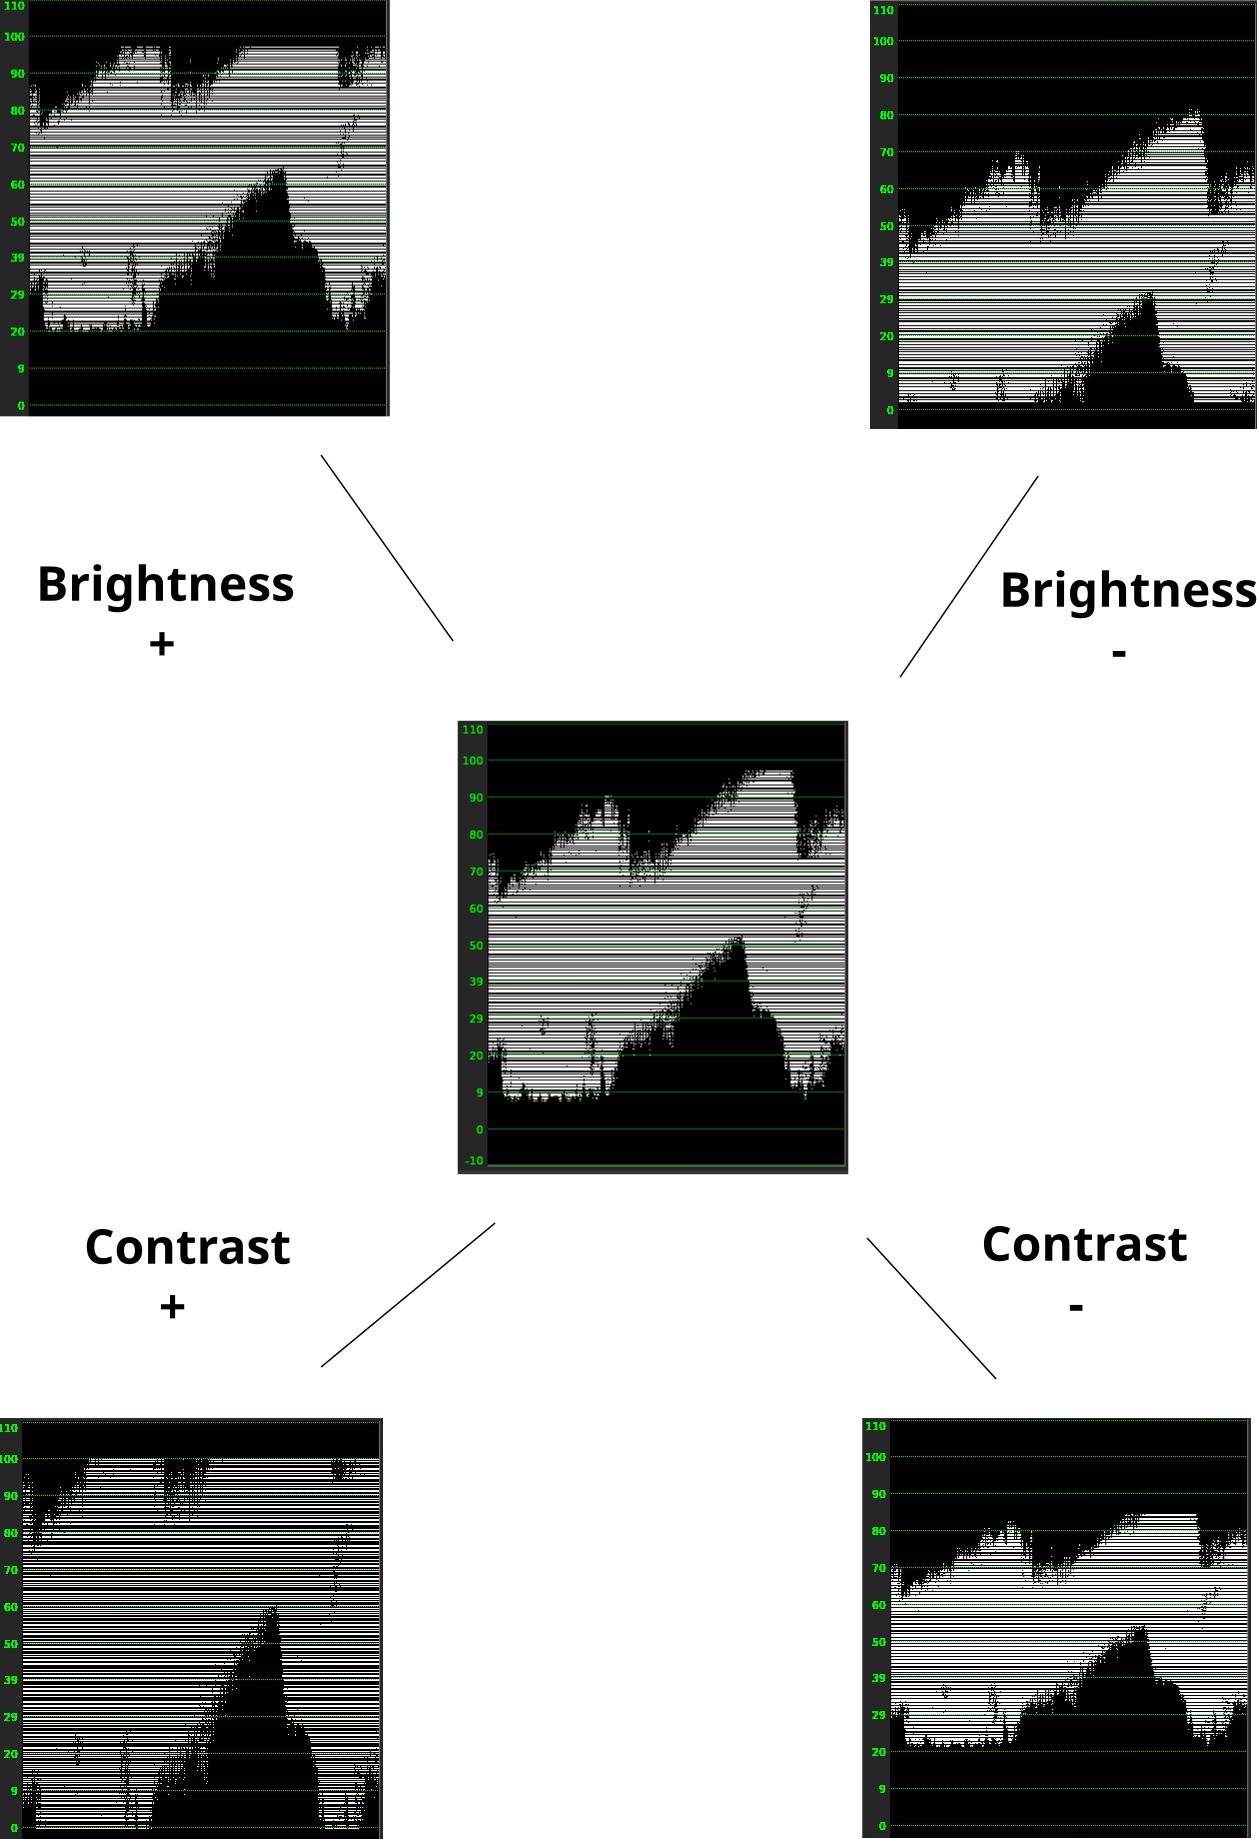
\includegraphics[width=0.6\linewidth]{brightness.png}
    \caption{How it works Brightness and Contrast}
    \label{fig:brightness}
\end{figure}

\subsection{BurningTV}%
\label{sub:burningtv}

Makes your video burn where there are small light colored patches of video. This came from \url{https://effectv.com}.

\subsection[C41]{C41\protect\footnote{credit Florent Delannoy, original program code author, and Edouard Chalaron}}%
\label{sub:c41}

The C41 plugin takes a $16\,bit C41$ digital intermediate negative film as input and outputs a positive image. It became necessary because $C-41$ negatives can fade or color-shift over time which was a problem early on. It is still important today because there is a large amount of documentaries, video clips, and other media out there that was shot on super $16$ film. This works for RGB-float, RGB, and also YUV variations.

There are two sets of data -- the scanned input values and your corrected values. Simple functionality of the plugin is to compute the data, transform to get corrected values, then apply that.

Basic usage strategy:
\begin{enumerate}
    \item first time the controls come up, nothing is checked and everything is set to $0$
    \item check the box \textit{Compute negfix values} to see the current media input values
    \item check \textit{Activate processing} and you see a $1-colored$ screen in the Compositor due to zero values
    \item check the \textit{Apply values box} to see the input values on the left side propagate to the right side
    \item check \textit{Apply default box} if you want to make sure that the borders of the image are not used
    \item correct the output values as desired on the applied right side
\end{enumerate}

It is important to note as you play or change the frame, the plugin re-computes the data as you move along, but it is not propagated to the applied side.


\paragraph{Checkboxes:}
    \begin{description}
        \item[Activate processing] when checked, the c41 operation is used to render the image.
        \item[Compute negfix values] computes the current negative values of the image (inside the box).
        \item[Show active area] draws horizontal and vertical grid lines displaying the boxed area.
        \item[Postprocess] when checked, applies contrast/brightness values as defined in $coef\frac{1}{2}$.
    \end{description}
\paragraph{Values:}
    \begin{description}
        \item[Compute negfix values] (left side) and
        \item[negfix values to apply] (right side):
        \item[Min/Max R/G/B] minimum and maximum values for Red, Green, and Blue.
        \item[Light] value of light; a smaller number is lighter.
        \item[Gamma G/B] values for gamma Green and Blue.
        \item[Contrast] simple color contrast.
        \item[Brightness] white brightness.
    \end{description}
\paragraph{Buttons:}
    \begin{description}
        \item[Apply values] copies computed RGB/Light/Gamma/Contrast/Bright from negfix to applied values.
        \item[Apply default box] copies default computed Box column/row from negfix to applied values.
    \end{description}
\paragraph{Shading box:} The boxing option allows for calculating the inversion of the digital negatives in a given area of the frame as opposed to the entire frame. The program will automatically calculate the columns and rows to shave from the frame when compute negfix values is checked. A default box area is initially calculated, called the shaving box, based on where the min/max difference in a row/column is less than the program defined tolerance. This row/column minimum and maximum difference must be greater than 0.05. The effect is to cut away the border areas with constant color. If you check the Show active area, you can see the box in the compositor window. The boundary search is constrained to a range of 0.1 to 0.9 times the frame dimensions, to create a 10 percent shaved margin to avoid over-scan and negative edge bleeding. Manual adjustment of the shaving box is controlled via the four sliders on the bottom right which move each of the left, right, top and bottom shaving margins. The slider bar new values automatically take effect as you move the box and you will see the right-hand side applied values change. When you have either the rows or the columns where the minimum slider is greater than or equal to the maximum slider, the default box will be in effect instead.

\paragraph{Optional postprocessing:} In order to have the values of Contrast and Brightness take effect, you must check the Postprocess checkbox.
\begin{description}
    \item[Contrast] is the difference in brightness between objects or regions.
    \item[Brightness] refers to the overall lightness or darkness of the image.
\end{description}

Figure~\ref{fig:c41} shows the C41 controls on the left and part of the Compositor window with grid lines showing the default shading box since the Show active area box is checked. Changes have been made to the left-hand side original computed values as seen in the right-hand side such as Gamma G which contains the hairline cursor and has a partial red outline value box.

\begin{figure}[htpb]
    \centering
    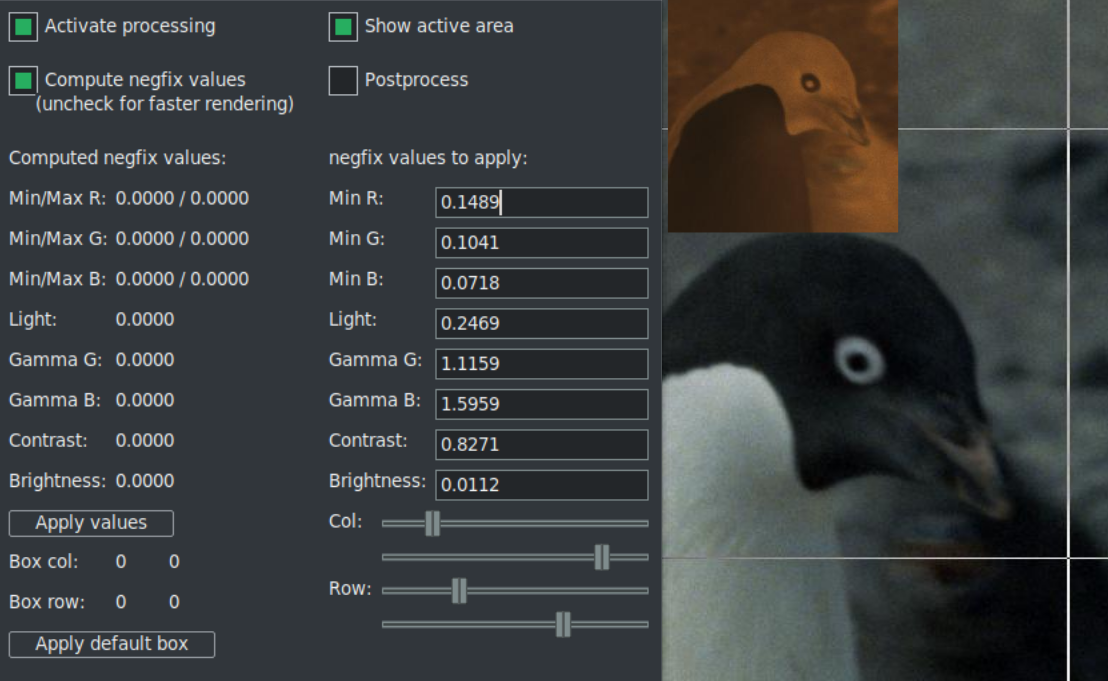
\includegraphics[width=0.9\linewidth]{c41.png}
    \caption{C41 - Control window and compositor window in action}
    \label{fig:c41}
\end{figure}

\subsection{Chroma Key}%
\label{sub:chroma_key}

This effect erases pixels which match the selected color. They are replaced with black if there is no alpha channel and transparency if there is an alpha channel. In this case, you create a matte in the alpha channel, which is not visible to us. The selection of color model is important to determine the behavior (figure~\ref{fig:chroma-key}).

\begin{figure}[htpb]
    \centering
    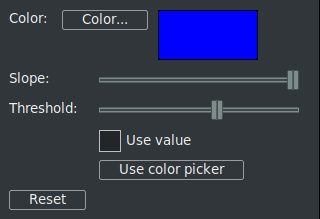
\includegraphics[width=0.5\linewidth]{chroma-key.png}
    \caption{Chroma Key control window}
    \label{fig:chroma-key}
\end{figure}

Chroma key uses either the \textit{lightness} or the \textit{hue} to determine what is erased. Use value singles out only the lightness to determine transparency.
Select a center color to erase using the \textit{Color} button. Alternatively a color can be picked directly from the output frame by first using the \textit{color picker} in the compositor window and then selecting the \textit{Use color picker} button. This sets the chroma key color to the current color picker color.

Be aware that the output of the chroma key is fed back to the compositor, so selecting a color again from the compositor will use the output of the chroma key effect. The chroma key should be disabled when selecting colors with the color picker.

If the lightness or hue is within a certain \textit{threshold} it is erased. Increasing the threshold determines the range of colors to be erased. It is not a simple on/off switch. As the color approaches the edge of the threshold, it gradually gets erased if the \textit{slope} is high or is rapidly erased if the slope is low. The slope as defined here is the number of extra values flanking the threshold required to go from opaque to transparent.

Normally threshold is very low when using a high slope. The two parameters tend to be exclusive because slope fills in extra threshold. The slope tries to soften the edges of the chroma key but it does not work well for compressed sources. A popular softening technique is to use a maximum slope and chain a blur effect below the chroma key effect to blur just the alpha.

\subsection[Chroma Key (HSV)]{Chroma Key (HSV)\protect\footnote{Credit for Plugin by Jerome Cornet \url{http://jcornet.free.fr/linux/chromakey.html}}}%
\label{sub:chroma_key_hsv}

Chroma Key (HSV) (figure~\ref{fig:chroma-key-hsv}) replaces a color with another color or transparency using HSV variables; it is frequently used to remove a color from a video to composite with another image. This process is generally referred to as green screen or blue screen process (because of the color that is keyed out). More information: {\small \url{http://en.wikipedia.org/wiki/Chromakey}}

\begin{figure}[htpb]
    \centering
    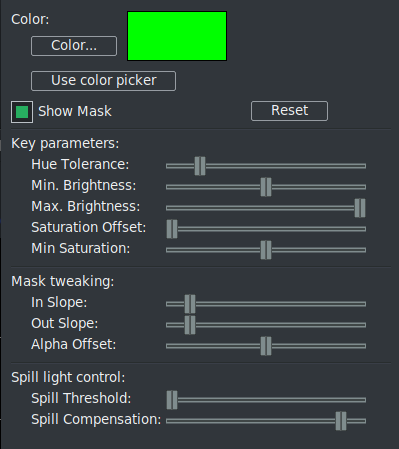
\includegraphics[width=0.55\linewidth]{chroma-key-hsv.png}
    \caption{Keying a green screen with Chroma Key (HSV)}
    \label{fig:chroma-key-hsv}
\end{figure}

\subsubsection*{Requirements}
\label{ssub:requirements}

The subject in the movie should have a good background. The lighting is crucial and good lighting during production will save you time with much less effort than in post-production.
Here we assume that we have a good video, filmed on green (or blue) screen that we want to use. Important: Make sure you are using a color model that has an alpha channel, such as \textit{RGBA8}, \textit{RGBAFloat}, \textit{YUVA8}. To change color model, go to \texttt{Settings $\rightarrow$ Format $\rightarrow$ Color Model}.

\subsubsection*{Usage}
\label{ssub:usage}

As in any other effect, add it to the timeline in the main window. You can tweak each parameter in order to improve the keying.

Start with \textit{Hue Tolerance} at $10\%$, \textit{Min Bright\-ness} at $0$, \textit{Max bright\-ness} at $100\%$, \textit{Saturation offset} at $0$, \textit{Min Saturation} at $0$, \textit{In Slope} at $0$, \textit{Out Slope} at $0$, \textit{Alpha Offset} at $0$ (that’s mid-way through), \textit{Spill Threshold} at $0$, \textit{Spill Compensation} at $100\%$. At any time, you can check what the Mask looks like by clicking on \textit{Show Mask}. This will output a black and white image of the mask (\textit{matte}).

\begin{description}
    \item[Key color:] Select the key color (green, blue, etc) using the color wheel or the color picker. Remember, only the Hue matters, not Saturation or Value. To use the color picker, click on the \textit{color picker} icon in the Compositor window, then click on the color you want in the Compositor window. Finally  in the Chromakey (HSV) parameters window, click on \textit{Use Color Picker}.
    \item[Hue Tolerance:] Because there are slight variations in lighting, the background will not be in a uniform key color hue. Increase or decrease the Hue tolerance to mask out the background. If there are dark spots that are keyed out that shouldn’t be, it can be corrected later.
    \item[Brightness:] ncrease \textit{Min Brightness} so that only the background is masked out, and not parts of the foreground. You can also reduce \textit{Max Brightness} if some clear areas are keyed out (useful for very dark backgrounds).
    \item[Saturation:] Increase \textit{Min Saturation} so that only the background is masked out, and not parts of the foreground. \textit{Saturation Offset} can be used to change this, but for now leave it set to $0$.
\end{description}

Check what it looks like at this stage, your mask should be pretty
clean. Toggle \textit{Show Mask} to check what it looks like, it
should be OK\@. If not, repeat steps $1 to 4$ to get a better
key. The rest of the controls are useful to smear the mask to help
compositing later on. They will help you to make your key look much
cleaner.

\begin{description}
    \item[Slope:] For now, the mask is a full on/ full off mask that can be really harsh and not necessarily what you are looking for. \textit{In Slope} and \textit{Out Slope} will help you to smooth that key. In Slope leaves more colors in the mask, Out Slope takes more colors out of the mask. The colors that are borderline in the mask will see their alpha channel reduced by half instead of being completely on or off.
    \item[Alpha Offset] This control offsets the whole alpha channel by some amount. Be sure to know what you are doing if you change it from the default value of $0$.
    \item[spill light control:] This step helps you remove the green or blue halo around the edges of the mask. It does so by removing the saturation of pixels that have a similar hue to the key color (turning them into grey instead of green or blue). \textit{Spill Compensation} controls the amount of de-saturation. If you start with Spill Compensation at $100\%$, slowly increase the \textit{Spill Threshold} until the remaining green or blue areas turn grey. Then reduce Spill Compensation until the image looks good.
\end{description}

Now the mask is probably still very harsh, so just below the Chromakey (HSV) plugin, add a \textit{Blur} effect, and select only the \textit{Alpha channel}, with a radius of $2$ or $3$ (more if you really want to soften the edges). This will significantly help the keying.

\subsection{Color 3 Way}%
\label{sub:color_3_way}

Together with \textit{Histogram Bezier / Curves} Color 3 Way is the main tool of Color Grading because you can modify the colors of \textit{Shadows}, \textit{Midtones}, and \textit{Highlights} as desired. Color 3 Way is keyframable (figure~\ref{fig:color3way}).

\begin{figure}[htpb]
    \centering
    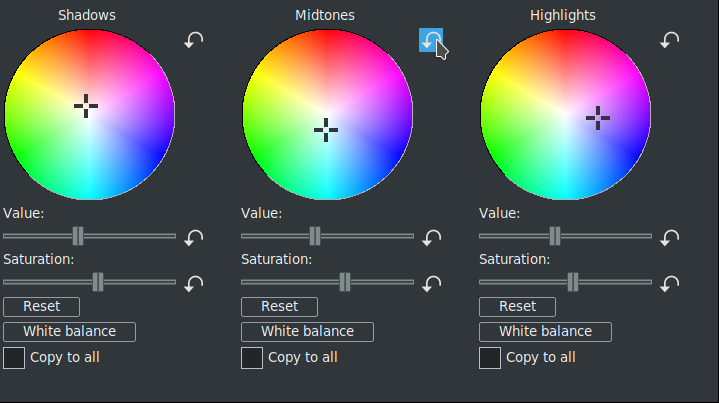
\includegraphics[width=1.0\linewidth]{color3way.png}
    \caption{Color 3 Way control window}
    \label{fig:color3way}
\end{figure}

\begin{itemize}
    \item It allows you to vary the \textit{contrast} of the image using the slider Value, always acting separately on shadows, midtones, and highlights and thus resulting in very precise application.
    \item Allows you to automate the \textit{white balance} by simply choosing a neutral color in the output of the Compositing window using the Color Picker and pressing the corresponding button in the plugin.
    \item Allows you to vary the \textit{Saturation} with sliders in the same manner as contrast was varied by the Value slider. For istance, to decrease the incidence of color dominants present in the shadows or in the highlights, vary the Saturation.
    \item With the \textit{color wheels} you can make very sophisticated adjustments to the shades of the images, in each of the three main areas of shadows, midtones and highlights.
    \item Allows you to copy exactly the setting of one zone to the other two zones using \textit{Copy to all} button.
    \item In addition to the three reset buttons, each slider and each wheel has its own Clear button, to return it to the default value without affecting the others.
\end{itemize}

This plugin allows maximum control over the result and maximum precision of adjustments when used simultaneously with the control monitors, i.e.\ \textit{Waveform}, \textit{RGB Parade} and \textit{Vectorscope}. It is important to keep in mind that the three zones are not clearly separated, but slightly overlapping. This results in less precision but looks better for more smooth shades. By varying the values on the color wheels all RGB channels are affected simultaneously, which can result in unwanted color dominance. Saturation is also affected and must therefore be monitored.
To use more precisely, drag the \textit{crosshair} with the mouse in the desired area and then adjust in steps of $0.001$ using the up/down and right/left arrows on the keyboard.
The most common use cases (but can be adapted to virtually any situation) of the plugin are:

\begin{itemize}
    \item White balancing.
    \item Expand/compress contrast.
    \item Mitigate under and over exposure.
    \item Balance colors, i.e.\ eliminate color dominance.
    \item Color matching Shot to Shot.
    \item Create a Stylized look.
\end{itemize}

\subsection{Color Balance}%
\label{sub:color_balance}

Video Color Balance is a great effect to use along with Brightness/Contrast and Hue/saturation to try to compensate for possible errors in filming (low lighting, for example). It can do so much without greatly lowering the quality of the video. With it you can change the colors being sent to output \textit{CMY} (Cyan, Magenta, Yellow) or \textit{RGB} (Red, Green, Blue). Color Balance is also keyframable.

Since \textit{complementary colors} are neutralized, to eliminate a \textit{color cast}, the pertinent slider is moved in the direction of the complementary color. Clear buttons are present to reset its slider to default without affecting others. If you \textit{Lock parameters} you get the same \textit{Color Offset}, that is the fourth color wheel in the grading programs. The parameters of the plugin are:

\begin{description}
    \item[CMY/RGB sliders:] allows you to adjust the colors.
    \item[Preserve Luminosity:] Adjusts colors while keeping the overall brightness constant.
    \item[Lock Parameters:] works as a Color Offset.
    \item[White Balance] used in conjunction with the \textit{color picker} on a neutral color of the output, it will automatically balance the white.
\end{description}

\subsection{ColorSpace}%
\label{sub:color_space}

This plugin is a tool that can be used to convert your input media, such as a recording from your camera,
from one color space/range to another.  It works for both RGB and YUV as set by your project format.
Options are BT601, BT709, or BT2020 for Color Space input and output and JPEG or MPEG for Color Range
input and output.  The Inverse option checkbox is available in case your media was rendered in the wrong
color space  or range so that you can fix it.

\textbf{Algorithm for conversion} -- where equations is a $3\times3$ matrix multiply

\qquad $output = (input - input\_zero) \times equations + output\_zero$

\textbf{Algorithm for inverse}  -- where equations is a $3\times3$ matrix multiply

\textit{Description}:    invert(equations); swap(input,output); swap(input\_zero,output\_zero)

\qquad $input = (output - output\_zero) \times inverse\_equations + input\_zero$

\begin{figure}[hbtp]
    \centering
    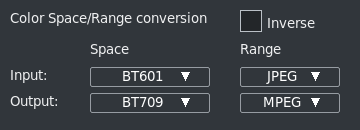
\includegraphics[width=0.6\linewidth]{colorspace.png}
    \caption{ColorSpace control window}
    \label{fig:colorspace}
\end{figure}


\subsection{CriKey}%
\label{sub:crikey}

The Chroma Interpolation Key plugin, CriKey, is a regionally based chroma key with interpolation (figure~\ref{fig:crikey}). This is useful when you only want 1 or some specific zones to be defined by the chroma key as opposed to the entire image. Its most significant feature is that you can select several regions of interests and of different colors as opposed to only $1$.

\begin{figure}[htpb]
    \centering
    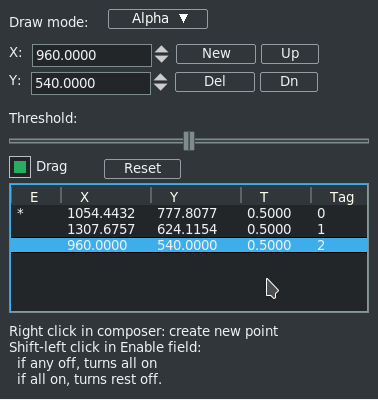
\includegraphics[width=0.5\linewidth]{crikey.png}
    \caption{three active point created in CriKey}
    \label{fig:crikey}
\end{figure}

To start, if not already checked, turn on drag. In the composer window select an area of a certain color by clicking on that point with the \textit{right mouse button} and check to see that it is enabled with an $*$ in the "E" field. The color of the area is used to define the region of interest and then you can use the \textit{threshold} slider to designate the tolerance variation. This creates a region that is the chroma key selection and a fill will be performed in that area, but only within that region. So, say for example, a red colored area was chosen, only the red color inside the region is selected -- not that color red in the entire image. The drag capability makes it easy to check a point before right clicking it to see the effect. You will want to turn off drag when you are finished with CriKey so that it does not interfere with other compositor functions.

\begin{description}
    \item[Draw mode:] options let you use \textit{Alpha} for see-thru, \textit{Edge} to just outline the edges of the region, or \textit{Mask} to block. The pixels which match the selected color are replaced by black if Mask is chosen or see-thru/transparent if Alpha.
    \item[X, Y:] points coordinate.
    \item[Buttons:] \textit{New} to create a new point, \textit{Up/Dn} to move highlighted point up or down \textit{Del} to delete the highlighted point.
    \item[Threshold:] slider goes from $0\, to\, 1$. Increasing the threshold, increases the area to be filled or masked. You can also use the mouse wheel to scroll the slider.
    \item[Drag:] for ease of use. If you need to clear the Drag enabled, you can easily do this with \textit{Allow keyframe spanning} whose use is described in \nameref{sec:allow_keyframes_spanning}.
    \item[Reset:] button to revert to only the default middle point with all others being deleted.
    \item[ListBox:] "E" for Enabled with $*$ marking that; "X" is the point’s $x$ coordinate; "Y" is the point’s $y$ coordinate; "T" is the threshold value of $X,Y$ point; \textit{Tag} represents the \# of the selected
    point.
    \item[Hints:] for usage shortcuts.
\end{description}

\subsubsection*{Some notable caveats}
\label{ssub:some_notable_caveats}

\begin{enumerate}
    \item When choosing an area that has variations of the same color within a region, for less work and for the best results, choose an average color in that region instead of an extreme end of that color.
    \item If the threshold is set appropriately you can see the edges which is helpful.
    \item The mask is computed and shows the fill region.
    \item Use the Gradient plugin to substitute a different color for the selected area.
\end{enumerate}

Figure~\ref{fig:crikey01} and figure~\ref{fig:crikey02} shows how moving the Threshold slider with the Point selected blacks out the single region which has the darker brown hills in it. Because the edge was located, any of the same color in the rest of the video would not be blacked out.

\begin{figure}[htpb]
    \centering
    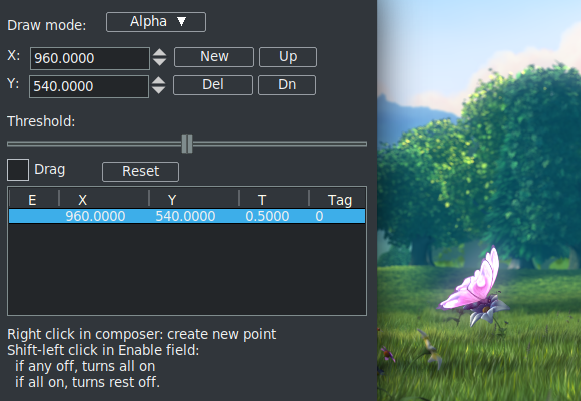
\includegraphics[width=0.7\linewidth]{crikey01.png}
    \caption{The screenshot shows the compositor with some default settings in the controls window.}
    \label{fig:crikey01}
\end{figure}

\begin{figure}[htpb]
    \centering
    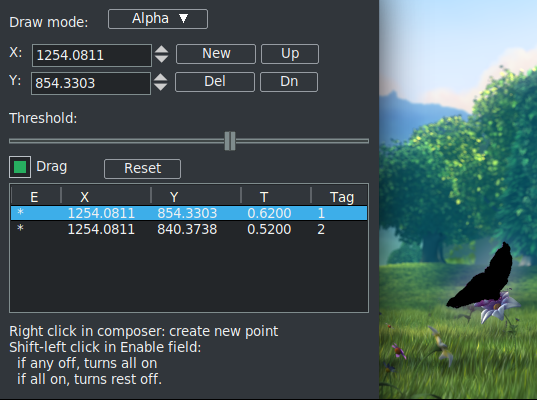
\includegraphics[width=0.7\linewidth]{crikey02.png}
    \caption{same screenshot with moving Threshold}
    \label{fig:crikey02}
\end{figure}

\subsubsection*{Usage steps}
\label{ssub:usage_steps}

\begin{enumerate}
    \item Click \textit{Reset} (there will be a single $X,Y$ coordinate point that is in the middle and not enabled)
    \item Check to make sure \textit{Drag} is on.
    \item In the Compositor, right click on area of interest and an $X,Y$ coordinate will appear in the listbox.
    \item Click on the \textit{E} Enabled field next to this latest point and an $*$ asterisk will show.
    \item Now you will see an area turn black so use the \textit{Threshold} slider to only black out the area of interest.
    \item Repeat steps $3-5$ until you have selected all of the desired areas.
    \item Finally, turn off \textit{drag} so as not to interfere with other compositor functions
\end{enumerate}

\subsection{Crop \& Position}%
\label{sub:crop_position}

It allows you to obtain a rectangle from the frame, whose dimensions are fully adjustable by four sliders for the four sides of the frame. You can also place this rectangle in the canvas using two other sliders for right/left and up/down scrolling. With the Clear buttons we can bring the slider to default values without affecting the other parameters. Unlike the \textit{Crop} tool, the original frame size is not altered and being keyframable allows a wide variety of uses. In figure~\ref{fig:crop_position} the Crop \& Position plugin is compared with the \textit{Crop} tool.

\begin{figure}[htpb]
	\centering
	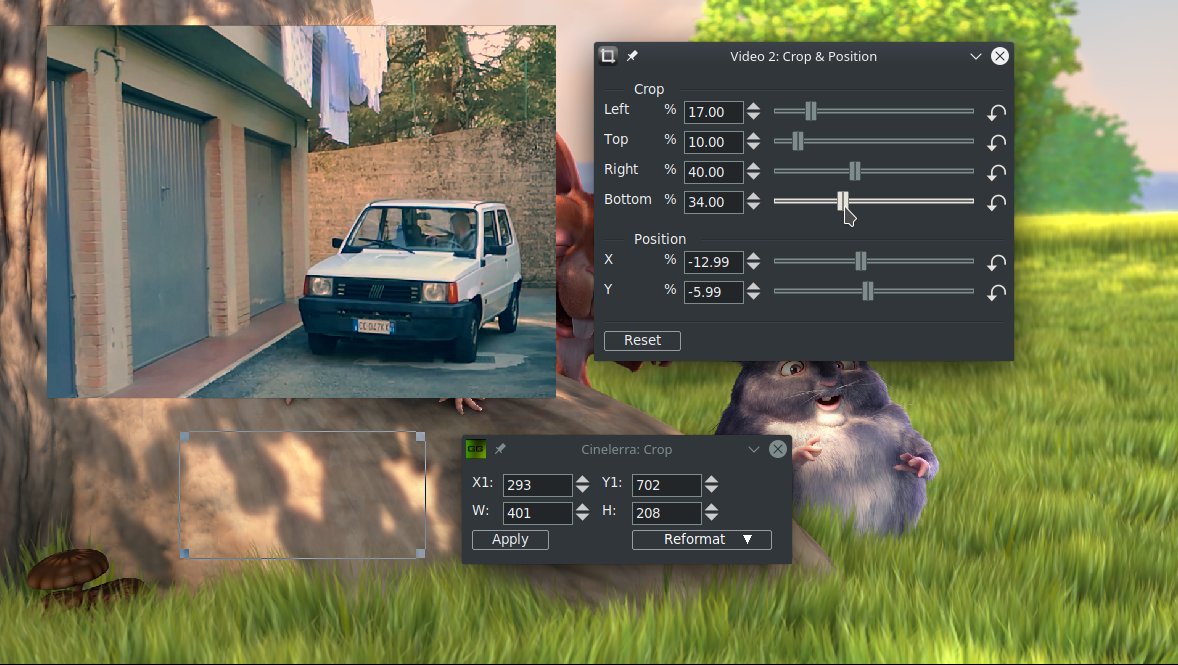
\includegraphics[width=1.0\linewidth]{crop_position.png}
	\caption{Crop tool and Crop \& Position plugin compared}
	\label{fig:crop_position}
\end{figure}

\subsection{DeScratch}%
\label{sub:descratch}

The descratch video plugin can be used to remove vertical scratches
from film. It can also be used, after image rotation, to remove
horizontal noise lines that may appear on analog \textit{VHS}
captures. For best results \textit{YUV} should be the video format;
however if your format is \textit{RGB}, it will first be converted
to YUV\@. There are many tuneable parameters necessary to get good
results for your specific film.

Figure~\ref{fig:descratch01} shows a list of the parameter descriptions:

\begin{figure}[htpb]
    \centering
    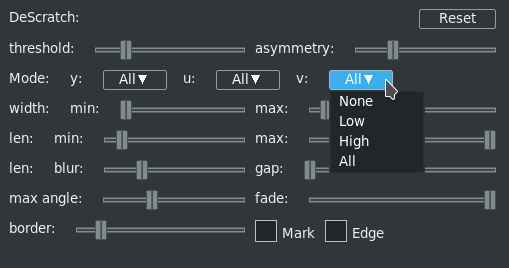
\includegraphics[width=0.6\linewidth]{descratch01.png}
    \caption{DeScratch control window}
    \label{fig:descratch01}
\end{figure}

\begin{figure}[htpb]
    \centering
    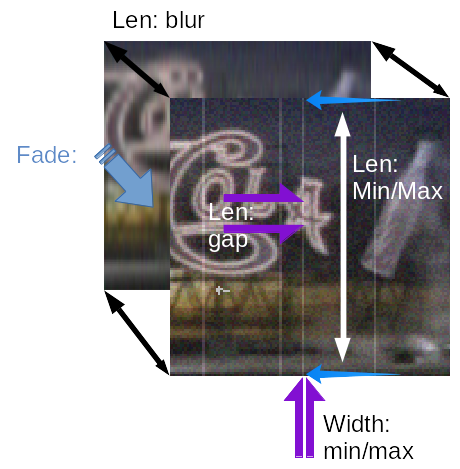
\includegraphics[width=0.5\linewidth]{descratch02.png}
    \caption{Various parameters of DeScratch}
    \label{fig:descratch02}
\end{figure}

\begin{description}
    \item[threshold] instantaneous slope value; chroma difference in numerical pixels.
    \item[asymmetry] maximum asymmetry of surrounding
    pixels.
    \item[Mode] \textit{None}; \textit{Low}=black; \textit{High}=white; \textit{All}=both;
    \textit{y} -- processing mode for \textit{luma} plane;
    \textit{u}-- processing mode for \textit{chroma u} plane;
    \textit{v} -- processing mode for \textit{chroma v} plane.
    \item[width min/max] minimal scratch width in pixels and maximum scratch width in pixels.
    \item[len min/max] percent minimal scratch length and percent maximum scratch length.
    \item[len blur] scaled radius of vertical blur for frame
    analysis.
    \item[len gap] number of pixels for maximum vertical gap
    to be closed.
    \item[max angle] maximal angle to vertical in degrees.
    \item[fade] percent of how much it fades to and how much it. Uses between before image and blurry image.
    \item[border] pixel thickness of border near scratch for partial restoration.
    \item[Mark] shows the potential scratch lines for ease of viewing and for debugging. It shows chosen pixels in the color green, close but still rejected in yellow, and extreme pixels in the color red. This makes it easy to vary some parameters to choose more or fewer scratch lines.
    \item[Reset] activating this button returns all of the parameters to their default values.
\end{description}

Figure~\ref{fig:descratch} shows a before and after DeScratch scenario. With \textit{Mark} set, you can see the black lines which indicate what the program was looking at to determine the scratches to remove.

\begin{figure}[htpb]
    \centering
    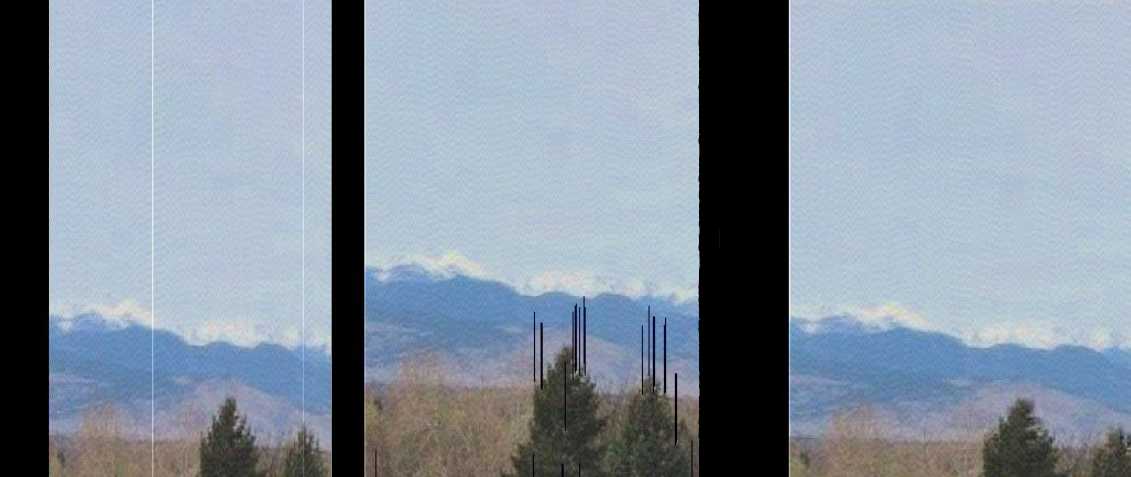
\includegraphics[width=0.9\linewidth]{descratch.png}
    \caption{Original video with scratch; Option Mark selected and Final video}
    \label{fig:descratch}
\end{figure}

\subsection{Decimate}%
\label{sub:decimate}

This is used to decrease the frame rate of a video. Changing the frame rate means eliminating a frame for any given number of frames ($1 in N$); but if frames that are important for visual continuity are deleted, temporal artifacts arise: flickering, slowdowns, accelerations, etc. The Decimate filter maintains a higher quality because it first eliminates duplicate frames or frames that are most similar, thus limiting the appearance of artifacts. It is often used after the \textit{Invert Telecine} plugin to make the video more smooth.

One use of the decimate effect can be applied to a DVD to convert the 29.97\,\emph{fps} video to the 23.97\,\emph{fps} film rate, but the effect can take any input rate and convert it to any lower output rate. The output rate of decimate is the project frame rate. The input rate is set in the decimate user interface. To convert 29.97\,\emph{fps} progressive video to 23.97\,\emph{fps} film, apply a decimate effect to the track. Set the decimate input rate to 29.97 and the project rate to 23.97.

Keep in mind that every effect layered before decimate, processes video at the decimate input rate and every effect layered after decimate, processes video at the project frame rate. Computationally intensive effects should come below decimate.

\subsection{Deinterlace}%
\label{sub:deinterlace}

The deinterlace effect has evolved over the years to deinterlacing and a whole lot more. In fact two of the deinterlacing methods, \textit{Inverse Telecine} and \textit{Frames to Fields}, are separate effects. The deinterlace effect offers several variations of line replication to eliminate comb artifacts in interlaced video. It also has some line swapping tools to fix improperly captured video or make the result of a reverse effect display fields in the right order.

\subsection{Deinterlace-CV}%
\label{sub:deinterlace_cv}

Selection of deinterlacing mode for your video to eliminate comb artifacts (figure~\ref{fig:deinterlace}).

\begin{figure}[htpb]
    \centering
    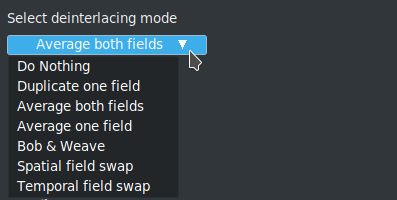
\includegraphics[width=0.6\linewidth]{deinterlace.png}
    \caption{Pulldown menu}
    \label{fig:deinterlace}
\end{figure}

\subsection{Delay Video}%
\label{sub:delay_video}

Delay the video by some number of seconds.

\subsection{Denoise Video}%
\label{sub:denoise_video}

Denoise video (figure~\ref{fig:denoise}).

\begin{figure}[htpb]
    \centering
    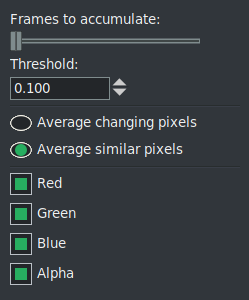
\includegraphics[width=0.4\linewidth]{denoise.png}
    \caption{Control window of the DeNoise plugin}
    \label{fig:denoise}
\end{figure}

\subsection{Difference key}%
\label{sub:difference_key}

The difference key creates transparency in areas which are similar between two frames. The Difference key effect must be applied to two tracks. One track contains the action in front of a constant background and another track contains the background with nothing in front of it. Apply the difference key to the track with the action and apply a \textit{shared effect} of it to the track with the background. The track with the background should be muted and underneath the track with the action and the color model should have an alpha channel. It’s hard to get good results.

Pixels which are different between the background and action track are treated as opaque. Pixels which are similar are treated as transparent. Change \textit{threshold} in the difference key window to make more pixels which are not the same color transparent. Change \textit{slope} to change the rate at which the transparency tapers off as pixels get more different. The slope as defined here is the number of extra values flanking the threshold required to go from opaque to transparent. A high slope is more useful with a low threshold because slope fills in extra threshold.
\textit{Use value} causes the intensity of pixels (\textit{luma}) to be compared instead of the color. Applying a \textit{blur} to the top track with just the alpha channel blurred can soften the transparency border (figure~\ref{fig:diff-key}).

\begin{figure}[htpb]
    \centering
    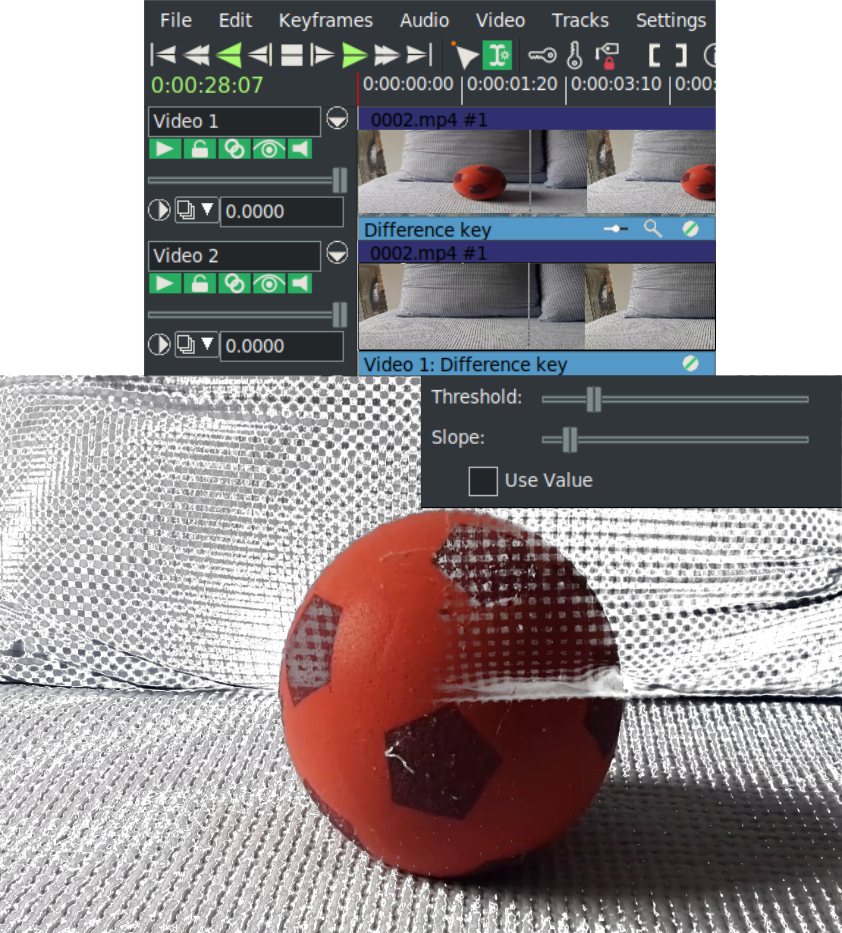
\includegraphics[width=0.8\linewidth]{diff-key.png}
    \caption{Difference key and its problematic output}
    \label{fig:diff-key}
\end{figure}

\subsection{DotTV}%
\label{sub:dottv}

Puts various size dots over the picture to simulate TV effect. This came from: {\small \url{https://effectv.com}}.

\subsection{Downsample}%
\label{sub:downsample}

Downsampling is the process of reducing the size of an image by throwing out data, reducing sampling rate.

\subsection{Edge}%
\label{sub:edge}

Display only the edges of the video throughout the image.

\subsection{Fields to frames}%
\label{sub:fields_to_frames}

See the theory description in the \textit{Frames to Fields} plugin. This effect reads frames at twice the project framerate, combining two input frames into a single interlaced output frame. Effects preceding fields to frames process frames at twice the project frame rate. Each input frame is called a field.

Fields to frames needs to know what field corresponds to what lines in the output frame. The easiest way to figure it out is to try both options in the window. If the input fields are the result of a line doubling process like frames to fields, the wrong setting results in blurrier output. If the input fields are the result of a standards conversion process like \textit{1080 to 480}, the wrong setting will not make any difference.

\subsection{Flip}%
\label{sub:flip}

This effect flips a video track either vertically or horizontally.

\subsection{Foreground}%
\label{sub:foreground}

Whatever the visual content of the frame, the Foreground plugin application applies a uniform color that can be chosen by color picker; color wheel; color presets; the various HSV, RGB, YUV sliders or by entering the hexadecimal value. The alpha slider is not missing either.

\subsection{Frames to fields}%
\label{sub:frames_to_fields}

\subsubsection*{Theory behind the Frames to Fields and Fields to Frames plugins}
\label{ssub:theory_frames_fields}

Historically, CRT-type TVs used interlaced signals to save bandwidth. An interlaced video consists of two \textit{fields} that are read and drawn on the screen one after the other. Each field must be played at a framerate double that of the resulting video. In two steps the complete frame will be reconstructed.

Frame 1 $\implies$ F1-field1 (\textit{Top} or \textit{Odd}), F1-field2 (\textit{Bottom} or \textit{Even})

Frame 2 $\implies$ F2-field1, F2-field2

Interlaced video reading: $F1-f1$ then $F1-f2$ then $F2-f1$ then $F2-f2$ \dots
There may be visual problems if the Top type interlacing is read according to a Bottom scheme. So it's important to know if a video is Top or Bottom. Generally an \textit{HD} video is Top; a \textit{DV} video (both PAL and NTSC) is Bottom; \textit{SD} (PAL) is Top; \textit{SD} (NTSC) is Bottom (but not always). Instead, high-definition videos need to be more compressed and this contrasts with the interlacing that is little and badly compressible, so modern videos are mostly \textit{progressive}.

\subsubsection*{In \CGG{}}
\label{ssub:in_cin_gg}

\begin{enumerate}
    \item upload an interlaced video to the Timeline and Resources and play it for viewing.
    \item The video presents visual artifacts because PC monitors are progressive.
    \item In the Resources window, open the media \textit{Info} with the right mouse button. Below you can see that the \textit{asset's interlacing} is active. It has four options for settings interlacing type: \textit{Unknown}, \textit{Top Fields first}, \textit{Bottom Fields first}, and \textit{Not interlaced}. If the file is (H)DV type, recognition and configuration is done automatically. All other media types will be set \textit{unknown}. We need to set the type of interlacing, so we have to manually set the interlacing.
    \item Now we can to use the \textit{Frames to Fields} plugin, but we have to configure it and act manually.
\end{enumerate}

Now for the practical use of this plugin which applies the operation reverse to the \textit{Fields to Frames} plugin. It extracts the two interlaced fields stored in alternating lines of interlaced source footage and outputs them as separate full frames. The alternating lines missing on each output frame are interpolated.

This plugin is only useful if its output is pulled with doubled framerate with respect to the source footage. One typical usage scenario is to do \textit{masking}, \textit{scaling} and \textit{translating} on interlaced footage without the need to destroy the additional temporal information contained in such source material. This is helpful if your intended target format is interlaced. If on the other hand, you just want to target a progressive display (for example, you create video for display on a computer monitor solely) then it is much more convenient to de-interlace the source material prior to any further processing.

\subsubsection*{Processing interlaced footage without deinterlacing}
\label{ssub:processing_interlace_footage}

\begin{enumerate}
    \item Create a new project with doubled frame rate. That is, make it $50\,fps$ if your source footage is $25i$.
    In \texttt{Resources $\rightarrow$ Media $\rightarrow$ Info} set the interlaced type (or unknown)
    \item Insert your source footage onto a video track in the timeline. Now, \CGG{} will playback each
    frame of your footage twice. There will be visual artifacts because the video is interlaced and the
    monitor is progressive.
    \item Apply the \textit{Frames to Fields} effect. Be sure to choose the correct field order. If we know or believe that the original video is \textit{Top First} let's try it first, but it doesn't have to be the right solution. The only way is to playback and look for visual artifacts.
    \item Then apply any further effects afterwards, including translations, scaling, slow motion, precise
    frame-wise masking or use of the motion tracker plugin.
    \item Render your project to an intermediate clip. Be sure to choose a rather lossless video codec, for
    example \textit{Motion-JPEG-A} or even \textit{uncompressed YUV} if you have plenty of storage.
    \item Insert the intermediate clip into your original project. Make sure the doubled framerate has been
    detected correctly by \CGG{} (by looking in the clip's media \textit{info} in the media resources folder).
    \item Apply the \textit{Fields to frames} effect to the intermediate clip. This will combine two adjacent fields
    into one interlaced field with the original frame rate.
    \item Do the final render on your original project. Now there will be no visual artifacts on the monitor.
\end{enumerate}

\subsection{Freeze Frame}%
\label{sub:freeze_frame}

In its simplest form, highlight a region of the track to freeze, drop the \texttt{freeze frame} effect on the highlighted region, and the lowest numbered frame in the affected area will play throughout the entire region. Freeze Frame has an enabled option which can be keyframed. Regions of a freeze frame effect which are enabled, repeat the lowest numbered frame since the last keyframe. This has unique possibilities.

\begin{itemize}
    \item If a freeze frame effect has a keyframe in the middle of it set to enabled, the frame in the middle is repeated in the entire effect.
    \item If a freeze frame effect has several keyframes, each set to enabled, every time a keyframe is encountered the frame under it becomes the frozen one.
    \item If a freeze frame effect alternates between enabled and disabled, each time an enabled keyframe is encountered the frame under it is replicated until the next disabled keyframe. The disabled regions play through.
\end{itemize}

\subsection{Gamma}%
\label{sub:gamma}

\textit{Log} camera images store colors in a $logarithmic$ scale. The blacks in these images are nearly $0$ and the whites are supposed to be infinity. The graphics card and most video codecs store colors in a $linear$ scale but \CGG{} keeps log camera images in their original logarithmic scale when it renders them. This is necessary because the raw image parser can not always decode the proper gamma ($\gamma$) values for the images. It also does its processing in $16\,bit$ integers, which takes away a lot of information.

Mathematically, the gamma function is exponential
($output = input^{\gamma}$) and therefore the inverse of the
logarithmic function [$output = \log(input)$]. Actually the formula
used by the \CGG{} plugin is: $output = input^{\frac{1}{\gamma}}$
which allows for a range of values $0 \div 1.0$. The gamma effect
converts the logarithmic colors to linear colors through a
\textit{gamma value} and a \textit{maximum value}. The gamma value
determines how steep the output curve is (i.e.\ the value of the
gamma parameter; for color space Rec709 is $2.4$
($\frac{1}{\gamma} =0.41\dots$), for sRGB is $2.2$
($\frac{1}{\gamma} =0.45\dots$), etc.). The maximum value is where
$1.0$ in the output corresponds to maximum brightness in the
input. It serves to avoid clipped values because it allows you to
set the maximum value of the output, $1.0$, whenever range
adjustment is done (see figure~\ref{fig:gamma01}). It is important
to adjust the two parameters accurately in order to avoid undesired
and unexpected effects, such as excessive values, unbalanced image,
incorrect linearization, etc.

\begin{figure}[htpb]
    \centering
    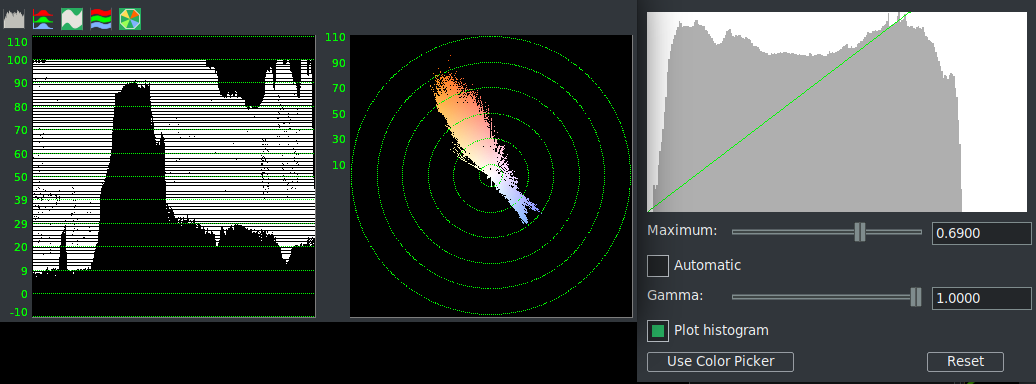
\includegraphics[width=1.0\linewidth]{gamma01.png}
    \caption{settting \textit{Maximun} to $0.6900$}
    \label{fig:gamma01}
\end{figure}

The gamma effect has two more parameters to simplify gamma correction. The automatic option causes it to calculate max from the histogram of the image. Use this when making a preview of a long list of images since it changes for every image. The use color picker option uses the value currently in the color picker to set the maximum value. Note that every time you pick a color from the compositor window, you need to click on use color picker to apply the new value.

The best use of the gamma is manually monitoring the waveform as shown in figure~\ref{fig:gamma02}.

\begin{itemize}
    \item Look at the highest peak on the \textit{waveform} and measure it with the crosshair observing the numerical value at the top left.
    \item Set this value with the \textit{maximum} slider.
    \item Then adjust the slider of the \textit{gamma} to our liking, always checking the result on the waveform so to be sure never to exceed the values of clipping, $0 \div 1.0$.
\end{itemize}

\begin{figure}[htpb]
    \centering
    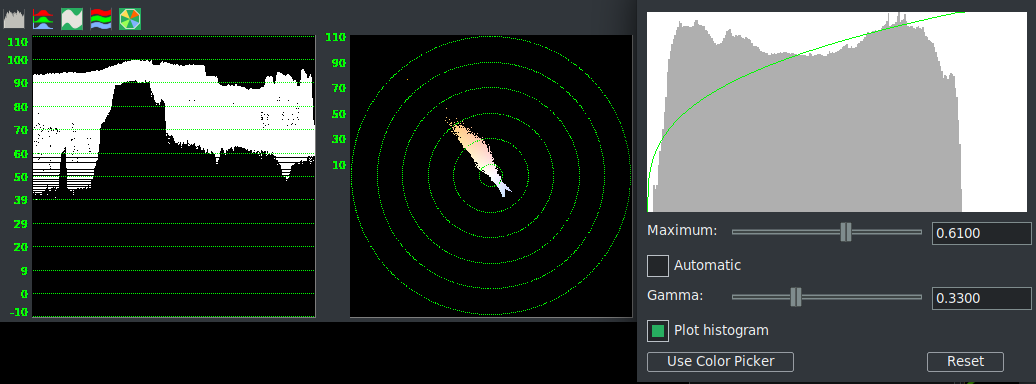
\includegraphics[width=1.0\linewidth]{gamma02.png}
    \caption{Setting \textit{Maximun} to $0.6100$ and \textit{Gamma} to $0.3300$}
    \label{fig:gamma02}
\end{figure}

Care must be taken when using gamma correction: if the image carries a specific gamma value, or if it has already been corrected previously (for example automatically in the camera), etc.; then a second application of the gamma leads to excessive and artificial results. Gamma is keyframable.

\subsection{Gradient}%
\label{sub:gradient}

The \textit{gradient} effect overlays a smooth color gradient on top of every video frame. It is useful for all sorts of background fills, for partially filtering, adding depth to the image, or for adding moving highlights. The Gradient effect can generate linear or circular color fills / shape. For linear fills, you can choose the \textit{angle}, for circular fills the \textit{center $(X,Y)$} of the created gradient pattern. You can control the \textit{slope} of the color transition by selecting a transition function ($linear$, $logarithmic$, $squared$) and by changing the start (\textit{inner}) and stop (\textit{outer}) radius. Note that both colors used in this color transition can contain an arbitrary \textit{Alpha} value (transparency). All parameters can be keyed and will be interpolated between keyframes.

The first time you use the plugin it may seem complicated, but if you understand that we have to adjust the gradient from an inner spot we choose to an outer spot we also choose, the work will become easy and fast.

\subsubsection*{Use case (Vignette)}
\label{ssub:use_case_vignette}

\begin{enumerate}
    \item Setting the shape to radial
    \item Setting the rate to Linear (or Log or Square)
    \item Position $X$ and $Y$ to center the main figure.
    \item Choose inner color=black
    \item Adjust inner radius
    \item Bring the inner color alpha slider to $0$
    \item Choose outer color=black
    \item Check that the outer color alpha slider is $1$.
    \item Adjust outer radius
\end{enumerate}

\textit{Note:} The inner and outer colors are visibly mixed in the gradient area. If you want to make a vignetting of only black, you must set the two colors to black and then make the inner one transparent so that it does not cover the figure.

\subsection{HistEq}%
\label{sub:histeq}

Remap colors using blended histogram weights. Figure~\ref{fig:histeq} shows the GUI and the results in a split screen.

\begin{figure}[htpb]
    \centering
    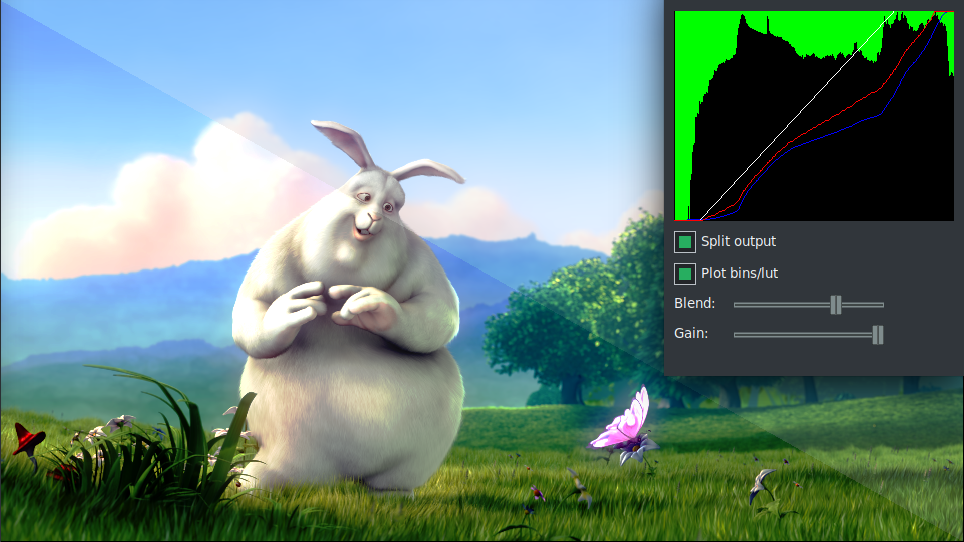
\includegraphics[width=0.8\linewidth]{histeq.png}
    \caption{Control window and split screen}
    \label{fig:histeq}
\end{figure}

Histeq equalizes the colorspace through use of a \textit{histogram equalization algorithm} -- a technique for adjusting image intensities to enhance contrast. Parameters are:

\begin{description}
    \item[Gain:] when set to $1$, the colorspace is best effort. If the gain is set to $0$, the result is the entire regression line of the color map.
    \item[Blend:] goes between a straight and a twisted line.
    \item[Split output:] diagonally shows in the compositor, the new results on the left and old on the right.
    \item[Plot bins/lut:] displays a plot of the result.
\end{description}

\subsection{Histogram}%
\label{sub:histogram}

The histogram allows an immediate view of the contrast amplitude of an image with its distribution of \textit{luma} and \textit{colors} values. If the columns of values occupy the whole range $0-100\%$ then we have maximum contrast; if the range is smaller the contrast is smaller. If most of the values are on the right of the histogram you have an image with highlights at the limit with values clamped to $1.0$. This is called \textit{overexposure}. However, if most of the values are moved to the left, with the limit of the values clamped to $0$, we have a lowlight image and we talk about \textit{underexposure}. Histogram is keyframble (figure~\ref{fig:histogram}).

\begin{figure}[htpb]
    \centering
    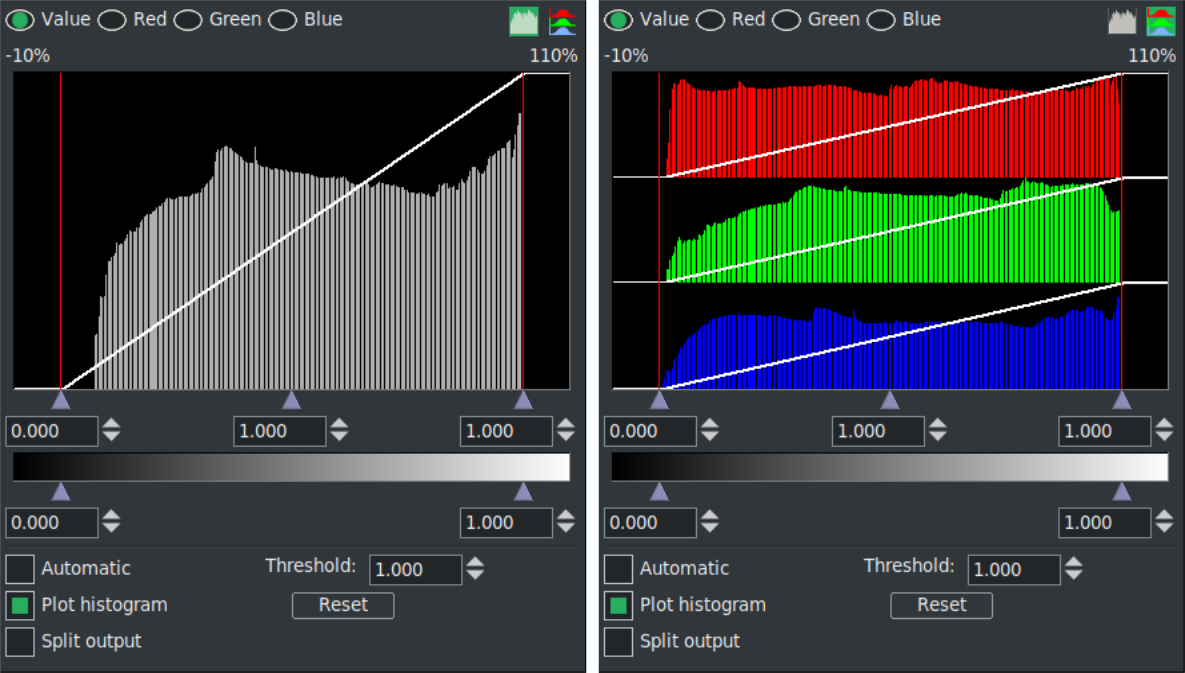
\includegraphics[width=0.9\linewidth]{histogram.png}
    \caption{Master Histogram and RGB Histogram}
    \label{fig:histogram}
\end{figure}

The Histogram is always performed in floating point RGB regardless of the project color space. The histogram has two sets of transfer parameters: the \textit{input transfer} and the \textit{output transfer}. The input transfer has value on the horizontal axis of $x$; it is a scale of values ranging from 0 to 255 in the case of an $8\,bit$ image, or it can have normalized values in the range ($0-1.0$) or even be a scale in percentage ($0-100\%$). In the output transfer (the $y\,axis$) is represented the number of times (that is, $y$) a given value $x$ appears. A higher column ($y$ greater) indicates that many pixels have the corresponding value $x$; a lower column indicates that fewer pixels have that value. On the left we have the minimum value $0$, which is the black point. On the right we have the maximum value $1.0$ which is the white point. The intermediate values pass smoothly from one extreme to the other. The three important points (including the midtones, i.e.\ the Master Offset) are indicated by cursors (small triangles) at the base of the histogram. You can adjust them to change the values of the three points if you want.

There are 4 possible histograms in the histogram viewer. The red, green, blue histograms show the input histograms for red, green, blue and multiply them by an input transfer to get the output red, green, blue. Then the output red, green, blue is scaled by an output transfer. The scaled red, green, blue is converted into a value and plotted on the value histogram. The value histogram thus changes depending on the settings for red, green, blue. The value transfers are applied uniformly to R, G, B after their color transfers are applied. Mathematically, it is said that the values of $x$ are linked to the values of $y$ by a transfer function. This function is represented by a line that leaves the values of $x$ and $y$ unchanged, but we can intervene by modifying this line with the cursors.

You need to select which transfer to view by selecting one of the channels on the top of the histogram. You can also choose whether to display the master, i.e.\ only the values of the \textit{luma}, or show the \textit{Parade}, i.e.\ the three RGB channels. You can switch from one to the other with the two buttons in the upper right corner. The input transfer is defined by a graph overlaid on the histogram; this is a straight line. Video entering the histogram is first plotted on the histogram plot, then it is translated so output values now equal the output values for each input value on the input graph.

After the input transfer, the image is processed by the output transfer. The output transfer is simply a minimum and maximum to scale the input colors to. Input values of $100\%$ are scaled down to the output's maximum. Input values of $0\%$ are scaled up to the output minimum. Input values below $0$ are always clamped to $0$ and input values above $100\%$ are always clamped to $100\%$. Click and drag on the output gradient's triangles to change it. It also has textboxes to enter values into.

Enable the \textit{Automatic} toggle to have the histogram calculate an automatic input transfer for the red, green, and blue but not the value. It does this by scaling the middle $99\%$ of the pixels to take $100\%$ of the histogram width. The number of pixels permitted to pass through is set by the \textit{Threshold} textbox. A threshold of $0.99$ scales the input so $99\%$ of the pixels pass through. Smaller thresholds permit fewer pixels to pass through and make the output look more contrasty.
\textit{Plot histogram} is a checkbox that enables plotting the histogram.
\textit{Split output} is a checkbox that enables a diagonal split showing in the compositor.
\textit{Reset} returns the four curves to their initial state (neutral) as well as the Value/RGB histogram buttons.

\subsection{Histogram Bezier / Curves}%
\label{sub:histogram_bezier_curves}

Histogram Bézier allows an immediate view of the contrast amplitude of an image with its distribution of luma and colors values using a piecewise linear method. In addition it uses a Bézier curve (parametric) on the histogram plot. When mapping color spaces, it has a variety of presentations to get smoother transitions and more pleasing output. It uses more general remapping, not just straight lines but more contour lines. Curves are perhaps the most powerful and sophisticated tool for color correction. For some repetitive details, see the previous description of the Histogram plugin. Histogram Bézier is keyframable.

The input graph is edited by adding and removing any number of points. Click and drag anywhere in the input graph to create a point and move it. Click on an existing point to make it active and move it. The active point is always indicated by being filled in. The active point's input X and output Y values are given in textboxes on top of the window. The input and output color of the point can be changed through these textboxes. Points can be deleted by first selecting a point and then dragging it to the other side of an adjacent point. They can also be deleted by selecting them and hitting delete (figure~\ref{fig:bezier}).

\begin{figure}[htpb]
    \centering
    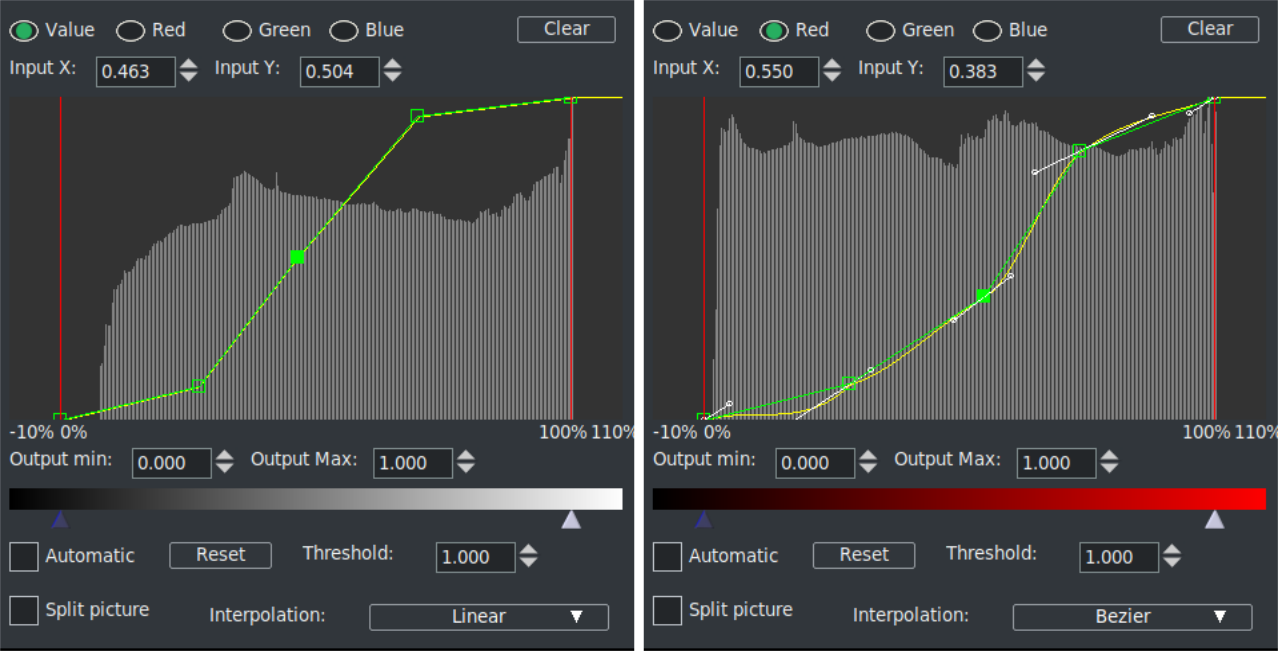
\includegraphics[width=0.9\linewidth]{bezier.png}
    \caption{Histogram Bezier / Curves}
    \label{fig:bezier}
\end{figure}

\begin{itemize}
    \item \textit{Master} (value) and \textit{R}, \textit{G}, \textit{B} histograms.
    \item Textbox for input $x$ (\textit{input}) and input $y$ (\textit{output}).
    \item \textit{Output min} and \textit{output max}: sets black or white points. If you use both points it works as Master/Color
    Offset. Values can also be less than $0$ and greater than $1.0$.
    \item Scale for \textit{contrast range}: sets with cursors shown as little triangles.
    \item \textit{Automatic} and \textit{Threshold}: enable the Automatic toggle to have the histogram calculate an automatic input transfer for the red, green, and blue but not the value. It does this by scaling the middle $99\%$ of the pixels to take $100\%$ of the histogram width. The number of pixels permitted to pass through is set by the Threshold textbox. A threshold of $0.99$ scales the input so $99\%$ of the pixels pass through. Smaller thresholds permit fewer pixels to pass through and make the output look more contrasty.
    \item \textit{Reset:} returns the four curves to their initial state (neutral).
    \item \textit{Split picture:} a checkbox that enables a diagonal split showing in the compositor.
    \item \textit{Interpolation:} type of algorithm for the parametric curves; linear, polynomial and Bezier.
\end{itemize}

Curves are used by introducing \textit{control points} simply with
the left mouse button and adjusting the value by dragging and
dropping. If you drag along the horizontal line only, you change the
value of $x$ and you can read this value in the input $x$
textbox. If you drag along the vertical line only, you change the
value of $y$ and you can read the value in the input $y$
textbox. This is the output value. The newly clicked control point
becomes active and is full green in color. To delete a point we have
to make it active and then press the Del key, or we can drag the
point beyond the position of another control point to its right or
left or, finally, pressing RMB\@. The control points corresponding to
the black point and the white point are automatically created from
the beginning, to fix their values and prevent clipping.

Curves are generally adjusted by introducing several control points, some to be kept fixed (as anchors) to prevent curve modification beyond them, and others to be dragged to make the desired correction. The power of the curves lies in being able to circumscribe a small interval at will and intervene only on this without involving the remaining parts of the frame. The precision with which you can work is such that you can almost arrive at a secondary color correction.

\begin{figure}[htpb]
    \centering
    \includegraphics[width=0.8\linewidth]{ex-bezier.png}
    \caption{Gain Up/Down; clamp; S-Shaped curve and Luma Key}
    \label{fig:ex-bezier}
\end{figure}


The most used type of modification is to create a \textit{S curve}. There can be a lot of shapes that use the S curve; the simplest is to create a control point in the shadows, one in the midtones (anchors) and one in the highlights. Moving the highlight point upwards and the shadow point downwards increases the contrast, making the image sharper and improving the color rendering. With the type of \textit{linear} curve you can make hard adjustments, similar to the result of the use of \textit{Color 3 Way}, even if this acts on the color wheel (Hue) while the curves act on individual RGB channels.

The \textit{Polynomial} and \textit{Bézier} types introduce \textit{control handles} that allow for more sophisticated and smoother adjustments. The quality of the result is much better, but they require more experience for their optimal use. Extending the handles away from the control point increases the \textit{radius} of the curve at that point. By varying the angle of the handles we change the \textit{tangent} and thus the curvature of the curve below. The difference between Polynomial and Bézier lies in the underlying mathematics, but for practical purposes the use is similar.

Some examples of the use of curves to demonstrate the variety of possible interventions (figure~\ref{fig:ex-bezier}):

\begin{itemize}
    \item Scale the image values by increasing the white point or decreasing the white point (gain up and gain down).
        You can decide the scaling value with the formula: $(Input \div Output) = Scale Factor$
    \item Limit a value beyond a certain point of brightness (clamp to the value $0.587$ in the figure).
    \item S-shaped curve to increase contrast without changing the black and white point (i.e.\ without \textit{clipping}).
    \item Make a real \textit{Luma Key} by bringing a certain value of gray to $100\%$ (white) and lowering everything else to $0\%$ (black). The slope of the two sides indicates how much we want to fade the edges of the matte obtained.
\end{itemize}

\subsection{HolographicTV}%
\label{sub:holographictv}

Incoming objects are projected like holovision seen in the movie Stars Wars as in R2-D2's video message projector of the Princess Leia. You need a movie or background image and above it a track containing the figure on which to apply the effect. This must have a transparent background. There are no configuration parameters; it only has to be applied to the upper track (figure~\ref{fig:holographictv}).

This effect originated from {\small \url{https://effectv.com}}.

\begin{figure}[htpb]
    \centering
    \includegraphics[width=0.8\linewidth]{holographictv.png}
    \caption{Holographic messages in CinGG!}
    \label{fig:holographictv}
\end{figure}

\subsection{Hue saturation}%
\label{sub:hue_saturation}

With this effect you can change hue, saturation and value. The parameters are modified using 3 simple sliders. The \textit{hue} control shifts the colors circularly in the color plane, normally resulting in false colors. The \textit{saturation} control can be used to reduce color footage to black and white. The \textit{value} control makes any given colors more bright or more subdued. Clear buttons are present to reset its slider to default without affecting others.

\subsection{Interpolate Bayer}%
\label{sub:interpolate_bayer}

Uses a Bayer filter algorithm to interpolate (estimate) missing color information. This is needed for some cameras where each pixel location only has an R or G or B value instead of all R, G, and B values for each location. The algorithm creates values for each of the three colors at every location by smearing (interpolating) each set of partial R, G and B values to create values at every pixel location.

\subsection{Interpolate Video}%
\label{sub:interpolate_video}

\subsubsection*{Theory}
\label{ssub:theory}

Each video has its own framerate. If we want to change it (for \textit{timelapse} or \textit{slowmotion}) the best thing is to shoot the scene with suitable framerate. But even in post production we can do something. The simplest method is to remove some frames to speed up the movie or add some to slow it down (from now on, for simplicity we will consider only the timelapse). Needless to say, the result is not smooth and the viewer will notice it immediately. A better method is to use the interpolation, mediating the pairs of frames that alternate. For example, if we have a sequence of frames $1, 2, 3, 4, 5, 6, 7, 8\dots$ we can make a timelapse mixing frames $1$ and $2$, $3$ and $4$, $5$ and $6$, $7$ and $8$ and so on. So we will have a new sequence of $4$ frames instead of the initial $8$: $\underline{12, 34, 56, 78}\dots$ We will get $50\%$ acceleration but it will always be of bad quality because of the too rough blending between the pairs of frames. Blending can be improved by weighing it differently by $50\% frame 1 + 50\% frame 2$, but the result is still unsatisfactory. Further improvements can be achieved by using $logarithmic$ or $exponential$ interpolation instead of $linear$ interpolation. But the most sophisticated methods that lead to better results are based on \textit{optical flow analysis}. These analyses the movement of circumscribed areas over a given period of time. With this method the intermediate frames do not derive from an approximate blending, but from the calculation of the \textit{vector} of the motion between two frames that determines the displacement (\textit{warping}) of the moving figure in the new intermediate frame. \textit{Interpolate Video} works this way.

\subsubsection*{Practice}
\label{ssub:practice}

The practical use of \textit{Interpolate Video} is a little different than the theory. The interpolate effect tries to create the illusion of a higher frame rate from source footage of very low framerates by averaging frames over time. It averages two input frames for each output frame. You choose a zone to be evaluated (\textit{macroblock size}) and a radius (\textit{search radius}) where you can search for this macroblock in the following frames. The \textit{Use optic flow} button is activated and playback starts. The plugin will calculate the motion vector (which can be made visible by the \textit{draw motion vectors} button) and apply it to intermediate frames. This operation is CPU intensive. Once the analysis is done, we can scroll the video by unchecking the two buttons and obtaining the desired result. There are two ways of specifying the input frames. You can specify an input frame rate which is lower than the project frame rate (\textit{imput frames per seconds}). This causes input frames to be taken at even intervals. You can also specify keyframe locations as the positions of the input frames (\textit{use keyframes as input}). In this mode the output frame rate is used as the input frame rate and you just create keyframes wherever you want to specify an input frame.

\subsection{Inverse Telecine}%
\label{sub:inverse_telecine}

This is the most effective deinterlacing tool when the footage is a video transfer of a film. This can be used to solve the problem, i.e., undo the damage caused by making film into a TV broadcast.
That process came about because film is at 24\,\emph{fps} while TV is at 29.97\,\emph{fps} and fields are at 60.
So the film was converted from 24\,\emph{fps} to 60\,\emph{fps}.
Roughly speaking, converting every 4 frames into 5 frames plus a slight slow down in speed.
Then the 60\,\emph{fps} was down-sampled to 30\,\emph{fps} by extracting odd and even lines and interlacing the lines.
This process is referred to as \textit{three-two pull down} ($3:2$ pull down) in filmmaking and television production for the post production process of transferring film to video.
The three-two pull down is where the telecine adds a third video field (a half frame) to every second video frame, but the untrained eye cannot see the addition of this extra video field.
The \texttt{IVTC} effect is primarily a way to convert \textit{interlaced} video to \textit{progressive} video.
It reverses the effect of three patterns of interlacing. In the next lines \texttt{A}, \texttt{B}, and \texttt{C} represent fields.

\texttt{A AB BC CD D}

\texttt{AB CD CD DE EF}

\texttt{Automatic}

The first two options are fixed patterns and affected by the pattern \textit{offset} and \textit{odd field first} parameters. The last option creates several combinations of lines for each frame and picks the most progressive combination. It is a brute force algorithm that is trying to resample the lines. This technique does not rely on a pattern like other techniques and is less destructive but the timing is going to be jittery because of the lack of a frame rate reduction. In order to smooth out the timing, you need to follow \textit{inverse telecine} with a \textit{decimate} effect.

\subsection{Invert Video}%
\label{sub:invert_video}

Invert video is a method of reversing the colors of a video track. The four parameters refer to channels -- \textit{Red}, \textit{Blue}, \textit{Green}, \textit{Alpha}. A very common use is to invert the alpha channel to change transparency.

\subsection{Lens}%
\label{sub:lens}

Create the effect of looking through a lens.

\begin{description}
    \item[R, G, B, A Field of View:] quantity of deformation of the relative fields. Often used with \texttt{Lock} to simultaneously affect the 4 fields.
    \item[Aspect Ratio:] determines the aspect ratio that you intentionally set.
    \item[Radius:] radius of curvature of the distortion. At minimum, it is a sphere (\textit{fish eye}) and at maximum, it is a rectangle (no distortion).
    \item[Center X, Y:] determines the coordinates of the center of the sphere. It can be made visible with \textit{Draw Center}.
    \item[Mode:] determines the type of distortion. The choice is between \textit{sphere shrink}, \textit{sphere stretch}, \textit{rectilinear shrink} and \textit{rectlinear stretch}.
    \item[Interpolation] determines the interpolation algorithm; from the fastest and least precise \textit{Nearest}, passing through \textit{BiLinear} to the better \textit{BiCubic}.
\end{description}

\subsection{Linear Blur}%
\label{sub:linear_blur}

This effect acts only in one direction which can vary up to an angle of $180\degree$ with these parameters:

\begin{figure}[htpb]
	\centering
	\includegraphics[width=0.8\linewidth]{linear.png}
	\caption{For clarity of presentation only 2 fields are shown}
	\label{fig:linear}
\end{figure}

\begin{description}
    \item[Lenght:] distance between original image and final blur step; corresponds to the distance of the fields.
    \item[Angle:] angle of motion in one direction for linear blur
    \item[Steps:] number of blur steps to be used in the calculation. Increasing the number takes more CPU.
    \item[Channels:] R,G,B,A.
    \item[Clear] With the Clear buttons we can bring the slider to default values without affecting the other parameters.
\end{description}

Figure~\ref{fig:linear} shown here has the parameters: $Length=19$, $Angle=25$, and $Steps=2$.

\subsection{Live Video}%
\label{sub:live_video}

This effect reads video directly from the capture card input. It replaces any video on the track so it is normally applied to an empty track. Only one \textit{Live Video} effect can exist at any time on the timeline. It can not be shared by more than one track. The configuration for the capture card is taken from the recording preferences. Go to \texttt{Settings $\rightarrow$ Preferences $\rightarrow$ Recording} to set up the capture card.

In the \textit{Video In} section where it says \textit{Record driver}, it should be set to either \textit{Video4Linux2} or \textit{IEC 61883}. Other video drivers have not been tested with Live Video and probably will not work. For live video, the selection for \textit{File} Format and \textit{Video} needs to be set to a format the timeline can use. The file format must be Quicktime for Linux and video recording must be enabled for it. Click on the wrench to set the video compression.

The video compression depends on the recording driver. For the \textit{Video4Linux2} recording driver, the compression must be \textit{Motion JPEG A}. For the \textit{IEC 61883} driver, the compression must be \textit{DV}. This gets the driver to generate output in a color model that the timeline can use. Some cards provide color and channel settings. Live video takes the color settings from the values set in the Video In window. Go to \texttt{File $\rightarrow$ Record} to bring up the recording interface and the Video In window. Values set in the Video in window are used by Live Video. Any channels the capture card supports need to be configured in the Video In interface since the same channels are used by the Live Video effect.

With the video recording configured, highlight a horizontal region of a video track or define in and out points. Then drop the Live Video effect into it. Drop other effects after Live Video to process the live video in realtime. For best results, you should use OpenGL and a video card which supports GL shading language. Go to \texttt{Settings $\rightarrow$ Preferences $\rightarrow$ Playback $\rightarrow$ Video Out} to enable the OpenGL driver.

\subsection{Loop video}%
\label{sub:loop_video}

Sections of video can be looped by dropping a loop effect on them. Contrary to the \texttt{settings $\rightarrow$ loop playback} option, the loop effects can be rendered where the \texttt{settings $\rightarrow$ loop playback} option can not be. The loop effects are also convenient for short regions.

The loop effects have one option: the \textit{number of frames} or \textit{samples} to loop. This specifies the length of the region to loop starting from either the beginning of the effect or the latest keyframe. The region is replicated for the entire effect.

Every time a keyframe is set in a loop effect, the keyframe becomes the beginning of the region to loop. Setting several keyframes in succession causes several regions to loop. Setting a single keyframe causes the region after the keyframe to be looped throughout the effect, no matter where the keyframe is. The end of an effect can be looped from the beginning by setting the keyframe near the end.

\subsection{Motion51}%
\label{sub:motion51}

This plugin compensates for unwanted motion and stabilizes the picture. The \textit{Motion51} Plugin simplifies motion stabilization so that without a lot of tweaking you can easily achieve reasonable results, either by using the defaults or varying a single parameter. Since the motion in every clip is specific, there are some additional parameters useful to adjust the settings accordingly. Alternatively, the \textit{MotionCV} and \textit{MotionHV} plugins can still be used as the originals, if more control over specific parameters is needed. The Motion51 plugin uses different methods for tracking than the other motion plugins. Motion Stabilization is very useful if you have jittery video, for example when taken from a car window, or while walking.

The better results require more samples. Setting the \textit{sample set size} is probably the most important setup change. Also, when computing motion compensation, the entire history of the image motion is important, and so it is desirable to enable the playback setting \textit{play every frame} in order to get good results. When every frame has to be processed, it can be time-consuming. Reasonable results are possible with small sample sets. After setup, the sample size can be increased to produce a high quality rendered result.

\subsubsection*{Description of what the program is doing}
\label{ssub:description_program_doing}

The motion is detected by \textit{sampling} the video image in a circular field. This size and placement of the sample region defaults to most of the image area. When the \textit{draw vectors} feature is enabled, the outer line trace encloses the searched region. The dotted circles define the target pixel set as the reference sample. The image is sampled using the circle pattern in a grid search. The best match is used to find the center and amount of rotation to transform the current image so that the reference area motion is canceled.

The amount of sampling does not significantly change for smaller or larger search areas. This means that a wide area can be searched just as easily as smaller areas. The main parameter which determines how hard it looks at the image is the \textit{samples} parameter. It represents the number of possible rotations, as well as the search precision. More samples mean more precision, and less jitter, but the program will run more slowly (figure~\ref{fig:motion51}).

\begin{figure}[htpb]
    \centering
    \includegraphics[width=0.9\linewidth]{motion51.png}
    \caption{Motion51 plugin window with its default options set.}
    \label{fig:motion51}
\end{figure}

The Samples box at the top is most often the only parameter that you may want to vary.

\subsubsection*{Program Parameters Description follows}
\label{ssub:program_parameters_description}

\begin{description}
    \item[X11-OpenGL:] setting can speed up the computation significantly in some cases when hardware OpenGL is available.
    \item[Samples:] is the number of pixels which the software will examine to stabilize the picture. The sample set is arranged in 4 equal concentric circular sets. Each sample dot represents content and position for a pattern matching test. Setting the samples to larger values improves the match by adding lots of placement possibilities. The samples/pixels that will be utilized are distributed throughout the selected area -- this is seen within the circles drawn when Draw Vectors is enabled. See figure~\ref{fig:motion51}.
    \item[Draw vectors:] demonstrates the search operation of motion stabilization. When enabled, the outer search boundary (oval), the search grid area (rectangle), and the reference sample (circles) are visible. 4 concentric circles show the reference sample set (target). You will also see an arrow in the center of the circle which shows each image displacement from frame to frame. When you render the video using the motion plugin, these dots/lines/circles are drawn into the rendered output. Draw vectors helps to visualize the meaning of the parameters to aid in setup. You should disable Draw Vectors before the final rendering.
    \item[Sample Radius:] is the radius of a circle that denotes the area of the sample locations. It is expressed as a percentage of the smallest image edge. For example, if it is set to $50\%$, then the circle will overlap about $\frac{1}{2}$ of the image. This does not change the number of samples. It does change the area from where the samples are gathered. If you have Draw vectors on, you can see the faint outline of a circle used for the radius.
    \item[Center X/Y:] is the center position of the sample circle, as a percentage of image width and height.
    This is useful to reset the reference focal point in cases where the important feature target is off-center.
    When both $X$ and $Y$ are set to $50\%$, the samples will be used from around the center of the video.
    \item[Search W/H:] determines the width and height of the rectangular area used for the grid pattern search. Samples are taken by moving the center of the circles in a grid pattern.
    \item[Horiz/Vert shake limit:] (Shaking refers to image translation) determines translation constraints. If the motion determined by the search exceeds the limit, it is clipped to a value that is at the limit boundary. For example, if the match indicates that the motion is $60\%$ off the reference target, but the limit is $50\%$, then the actual translation used will be limited to only $50\%$.
    \item[Shake fade:] determines how fast the translation cancellation fades away, and the image resettles to its actual appearance. Every frame that is processed accumulates the motion of the past. The amount of the past motion which is applied is reduced by the fading factor. The current match is then added to the fading past motion history. Fading works fast. It is applied every frame. So if fade is $10\%$, and no new motion occurs in the input, the history will be $90\%, 81\%, 73\%, 66\%\dots$ and in $30$ frames only $4.2\%$ of the past motion will be present in the effect. Fading insures that the image will eventually settle re-centered when the image motion ends.
    \item[Twist limit:] (Twisting refers to image rotation) determines the rotation constraints. If the rotation determined by the search exceeds the limit, it is clipped to the limit boundary. Its operation is similar to the shake limits.
    \item[Twist fade:] determines how fast the rotation cancellation fades away, and the image resettles to its actual appearance. Its operation is similar to the shake fade.
    \item[Enable Tracking:] caches the search results in a file so that subsequent playback does not have to be recalculated. When tracking is enabled, before a frame is processed the frame number is used to look for cached results. If cache data is available, it is used. If no data is available, the frame is processed by the motion tracking search, and the results are added to the cache file. If tracking is not enabled, the data is always sourced from the motion tracking search and the tracking file is not updated.
    \item[Tracking file:] is the name of the file which will contain the calculated values to be saved. Note that the default is \texttt{/tmp/motion51} which can be hazardous, since a system crash or a reboot can delete \texttt{/tmp} files.
    \item[Reset Defaults:] button is used to revert to the initial defaults built into the program.
    \item[Reset Tracking:] will delete the current Tracking file and disables tracking so that any previously calculated values are no longer available. However, because motion stabilization can often be cpu intensive, if the default file already exists, it will create a file name from the loaded asset.
    \item[Play Every Frame:] shows if you are Currently using: Play every frame. For best results, set play every frame. This can be set in \texttt{Settings $\rightarrow$ Preferences $\rightarrow$ Playback A} Tab in the \textit{Video out} section.
\end{description}

\subsection{Motion}%
\label{sub:motion}

The \textit{motion tracker} is almost a complete application in itself. The motion tracker tracks two types of motion: \textit{translation} and \textit{rotation}. It can track both simultaneously or one only. It can do $\frac{1}{4}$ pixel tracking or single pixel tracking. It can stabilize motion or cause one track to follow the motion of another track. Although the motion tracker is applied as a realtime effect, it usually must be rendered to see useful results. The effect takes a long time to precisely detect motion so it is very slow.

Motion tracker works by using one region of the frame as the region to track (Match Box). It compares this region between $2$ frames to calculate the motion. This region can be defined anywhere on the screen. Once the motion between $2$ frames has been calculated, a number of things can be done with that \textit{motion vector}. It can be scaled by a user value and clamped to a maximum range. It can be thrown away or accumulated with all the motion vectors leading up to the current position.

To save time the motion result can be saved in a file for later reuse, recalled from a previous calculation, or discarded. The motion tracker has a notion of $2$ tracks, the \textit{master} layer and the \textit{target} layer. The master layer is where the comparison between $2$ frames takes place. The target layer is where motion is applied either to track or compensate for the motion in the master layer.

Motion tracking parameters:

\begin{description}
    \item[Track translation] Enables translation operations. The motion tracker tracks $X$ and $Y$ motion in the master layer and adjusts $X$ and $Y$ motion in the target layer.

    \item[Translation block size] For the translation operations, a block is compared to a number of neighboring blocks to find the one with the least difference. The size of the Match Box to search for is given by this parameter.
    \item[Translation search radius] The size of the area to scan for the translation block.
    \item[Translation search steps] Ideally the search operation would compare the translation block with every other pixel in the translation search radius. To speed this operation up, a subset of the total positions is searched. Then the search area is narrowed and re-scanned by the same number of search steps until the motion is known to $\frac{1}{4}$ pixel accuracy.
    \item[Block X, Y] These coordinates determine the center of the translation block based on percentages of the width and height of the image. The center of the block should be part of the image which is visible at all times.
    \item[Maximum absolute offset] The amount of motion detected by the motion tracker is unlimited if this is $100$. If it is under $100$ the amount of motion is limited by that percentage of the image size.
    \item[Settling speed] The motion detected between every frame can be accumulated to form an absolute motion vector. If the settling speed is $100$ the absolute vector is added to the next frame. If the settling speed is less than $100$ the absolute vector is downscaled by the settling amount before being added to the next frame.
    \item[Track rotation] Enables rotation operations. The motion tracker tracks rotation in the master layer and adjusts rotation in the target layer.
    \item[Rotation block size] For rotation operations a single block is compared to equally sized blocks, each rotated by a different amount. This is the size of the rotation block.
    \item[Rotation search radius] This is the maximum angle of rotation from the starting frame the rotation scanner can detect. The rotation scan is from this angle counterclockwise to this angle clockwise. Thus the rotation search radius is half the total range scanned.
    \item[Rotation search steps] Ideally every possible angle would be tested to get the rotation. To speed up the rotation search, the rotation search radius is divided into a finite number of angles and only those angles compared to the starting frame. Then the search radius is narrowed and an equal number of angles is compared in the smaller radius until the highest possible accuracy is achieved. Normally you need one search step for every degree scanned. Since the rotation scanner scans the rotation search radius in two directions, you need two steps for every degree in the search radius to search the complete range.
    \item[Draw vectors] When translation is enabled, $2$ boxes are drawn on the frame. One box represents the translation block. Another box outside the translation block represents the extent of the translation search radius. In the center of these boxes is an arrow showing the translation between the $2$ master frames. When rotation is enabled, a single box the size of the rotation block is drawn rotated by the amount of rotation detected.
    \item[Track single frame] When this option is used the motion between a single starting frame and the frame currently under the insertion point is calculated. The starting frame is specified in the Frame number box. The motion calculated this way is taken as the absolute motion vector. The absolute motion vector for each frame replaces the absolute motion vector for the previous frame. Settling speed has no effect on it since it does not contain any previous motion vectors. Playback can start anywhere on the timeline since there is no dependence on previous results. We talk about \textit{Keep shape} and it is the most precise way to calculate the motion vector; but it only works well when the object to be traced does not change along the clip, remaining identical in shape, size and without rotation.
    \item[Track previous frame] Causes only the motion between the previous frame and the current frame to be calculated (\textit{Follow shape}). This is added to an absolute motion vector to get the new motion from the start of the sequence to the current position. After every frame processed this way, the block position is shifted to always cover the same region of the image. Playback must be started from the start of the motion effect in order to accumulate all the necessary motion vectors. This method is less precise because you have error propagation between frames. However, it is essential when the object changes shape or size or rotates.
    \item[Previous frame same block] This is useful for stabilizing jerky camcorder footage. In this mode the motion between the previous frame and the current frame is calculated. Instead of adjusting the block position to reflect the new location of the image, like Track Previous Frame does, the block position is unchanged between each frame. Thus a new region is compared for each frame.
    \item[Master layer] This determines the track which supplies the starting frame and ending frame for the motion calculation. If it is Bottom the bottom track of all the tracks sharing this effect is the master layer. The top track of all the tracks is the target layer.
    \item[Calculation] This determines whether to calculate the motion at all and whether to save it to disk. If it is \textit{Don't Calculate} the motion calculation is skipped. If it is \textit{Recalculate} the motion calculation is performed every time each frame is rendered. If it is \textit{Save} the motion calculation is always performed but a copy is also saved. If it is \textit{Load}, the motion calculation is loaded from a previous save calculation. If there is no previous save calculation on disk, a new motion calculation is performed.
    \item[Action] Once the motion vector is known this determines whether to move the target layer opposing the motion vector or following the motion vector. If it is \textit{Do Nothing} the target layer is untouched. If it is \textit{Track\dots} the target layer is moved by the same amount as the master layer. This is useful for matching titles to objects in the frame. If it is \textit{Stabilize\dots} the target layer is moved opposite to the motion vector. This is useful for stabilizing an object in the frame. The motion operations can be accurate to single pixels or subpixels by changing the action setting.
\end{description}

\subsubsection*{Secrets of motion tracking}
\label{ssub:secrets_motion_tracking}

Since it is a very slow effect, there is a method to applying the motion tracker to get the most out of it. First disable playback for the track to do motion tracking on. Then drop the effect on a region of video with some motion to track. Then rewind the insertion point to the start of the region. \textit{Set Action $\rightarrow$ Do Nothing}; \textit{Set Calculation $\rightarrow$ Don't calculate}; Enable \textit{Draw vectors}. Then enable playback of the track to see the motion tracking areas.

Enable which of translation motion or rotation motion vectors you want to track. By watching the compositor window and adjusting the \textit{Block x,y} settings, center the block on the part of the image you want to track. It is advisable to choose elements that have evident edges in the $x$ and $y$ directions because the calculations are made on these coordinates. Then set \textit{search radius}, \textit{block size} and \textit{block coordinates} for translation and rotation.

Once this is configured, set the calculation to \textit{Save coords} and do test runs through the sequence to see if the motion tracker works and to save the motion vectors. Next, disable playback for the track, disable \textit{Draw vectors}, set the motion action to perform on the target layer and change the calculation to \textit{Load coords}. Finally enable playback for the track.

When using a single starting frame to calculate the motion of a sequence (Keep Shape), the starting frame should be a single frame with the least motion to any of the other frames. This is rarely frame $0$. Usually it is a frame near the middle of the sequence. This way the search radius need only reach halfway to the full extent of the motion in the sequence.

If the motion tracker is used on a render farm, Save coords and previous frame mode will not work. The results of the save coords operation are saved to the hard drives on the render nodes, not the master node. Future rendering operations on these nodes will process different frames and read the wrong coordinates from the node filesystems. The fact that render nodes only visualize a portion of the timeline also prevents previous frame from working since it depends on calculating an absolute motion vector starting on frame $0$.

\subsubsection*{2 pass motion tracking}
\label{ssub:2_pass_motion_tracking}

The method described above is \textit{two-pass motion tracking}. One pass is used just to calculate the motion vectors. A second pass is used to apply the motion vectors to the footage. This is faster than a single pass because errors in the motion vector calculation can be discovered quickly. This also allows the motion tracking to use a less demanding colormodel like \textit{RGB888} in the scanning step and a more demanding colormodel like \textit{RGB Float} in the action step. The scanning step takes much longer than action. This has the disadvantage of not being practical for extremely long sequences where some error is acceptable and the picture quality is low to begin with, like stabilizing camcorder footage.

The slower method is to calculate the motion vectors and apply them simultaneously. This method can use one track as the motion vector calculation track and another track as the target track for motion vector actions. This is useful for long sequences where some error is acceptable.

\subsubsection*{Pre-processing the shot}
\label{ssub:pre_processing_shot}

\begin{enumerate}
    \item The motion plugin uses \textit{luminance} to do its own calculations, so we can edit the clip to enhance contrast and make it easier to calculate motion vectors. You can even create a copy of the monochrome clip and optimize it for the plugin. It lengthens the time but minimizes errors. The saved file can then be used for the original clip.
    \item  Correct lens distortion, especially if the object to be tracked moves to the edges of the frame.
    \item Study the entire shot well: if necessary, divide it into many edits, each with its own Motion plugin. For example, if the object to be tracked leaves the frame or is covered by some other element or changes in shape, size or rotation. You can try to use the \textit{Offset Tracking} technique described below.
\end{enumerate}

\subsubsection*{Using blur to improve motion tracking}
\label{ssub:blur_improve_motion_tracking}

With extremely noisy or interlaced footage, applying a blur effect before the motion tracking can improve accuracy. Either save the motion vectors in a tracking pass and disable the blur for the action pass or apply the blur just to the master layer. You can even use a copy of the track formed only by the channels of Red + Green, because the channel of Blue is the noisiest. Another trick is to enlarge the Match Box to minimize the effect of noise.

\subsubsection*{Using histogram to improve motion tracking}
\label{ssub:histogram_improve_motion_tracking}

A histogram is almost always applied before motion tracking to clamp out noise in the darker pixels. Either save the motion vectors in a tracking pass and disable the histogram for the action pass or apply the histogram just to the master layer. Finally, you can use the histogram to increase contrast.

\subsubsection*{Possible sources of errors}
\label{ssub:possible_sources_errors}

\begin{description}
    \item[Search radius too small:] the traced object moves too fast with respect to the size of the search box set.
    \item[Search radius too large:] The search box is so large that it also collects other similar items in the frame.
    \item[Occlusions:] the traced object is temporarily hidden by some other element. \textit{Offset tracking} or splitting of the video into several homogeneous clips is required.
    \item[Focus change:] you may get errors if the object changes its focus. The video must be divided into several homogeneous clips.
    \item[Motion Blur:] blurs the object making the calculation of the motion vector less precise. Very little can be done.
    \item[Shape change:] you can use \textit{Track previous frame} or the subdivision of the video in more homogeneous clips.
    \item[Lighting change:] Contrast change can produce errors. \textit{Track previous frame} or color correction can be used to return to the initial illumination.
\end{description}

\subsubsection*{Tracking stabilization in action}
\label{ssub:tracking_stabilization_action}

This is an explanation of how to stabilize a video as in the case of a video taken from a vehicle.

First select on the timeline the part of the footage you want to stabilize, using the in and out points. Then apply the motion effect on that part of the video. Select the \textit{Previous frame same block} option. That option is recommended for stabilizing jerky camcorder footage. Its goal is not to \textit{follow} an object. The block stays exactly at the same place during all the effect length.

Enlarge the block and select almost half the size of the video. Select the \textit{Stabilize subpixel} option as it will give a finer stabilization. Reduce the \textit{Maximum absolute offset} value to limit the stabilization amplitude. You probably prefer to get a non-perfect stabilization on some places on the video rather than having a very large black border on one side of the picture during big shakes. Set the \textit{Translation search steps} value to $128$. Increasing that value will not give a better result and only considerably increases the rendering time. Make sure the \textit{Draw vectors} option is selected, and render the part of the video where the motion effect is applied.

If the result is good, deselect the \textit{Draw vectors} option so that the block and vectors are not drawn anymore on the video. Then, render your video to a \texttt{.dv} file, and import it into your project. You will notice the video is stabilized but there are black borders which appear on sides of the frame. You have to \textit{zoom in} and define projector keyframes to move the projector around the screen, in order to remove those black borders. The more your footage is jerky, the more you have to zoom in to discard the black borders. That is why the result is better with HDV footage than with DV footage.

An interesting side note about \textit{add offset} usage is explained next\protect\footnote{credit Pierre Marc Dumuid}

To stabilize video, the motion plugin uses a \textit{tracking frame} to which to track to and a region within that frame to track (generally an object in the background) in the current frame.  When the region is obscured, often by something in the foreground or by leaving the screen, then the motion compensation would fail, and the video jumps all over the place.

You set a second region to track, and then \textit{add offset}.

This shows how it is used.  It works very well:

\begin{verbatim}
------k-------k-----------------
^      ^^
A      BC

A - object1 is visible in the background up until C
B - (the frame before C) has both object1 and object2 visible
C - has only object2 visible
\end{verbatim}

\begin{enumerate}
    \item Make a keyframe and set to track object1.
    \item Make a keyframe at C and track frame at B, set to track object2.
    \item Set keyframe at C to add offsets that were calculated at B.
\end{enumerate}

\subsubsection*{Tips}
\label{ssub:tips}

\begin{enumerate}
    \item The motion vector is a text file located in \texttt{/tmp}. We can open it with a plain editor and modify the wrong $X\,Y$ coordinates, i.e.\ those that deviate from the linearity, to correct the errors that always happen when we perform a motion tracking (jumps). It can be a long and tedious job, but it leads to good results.
    \item You can try tracking using reverse playback of the track. Sometimes it may lead to a better calculation.
\end{enumerate}

\subsection{Motion 2 Point}%
\label{sub:motion_2_point}

Motion stabilization using 2 pass tracking. For theory and explanations refer to the \hyperref[sub:motion]{Motion} plugin.

\subsection{Motion Blur}%
\label{sub:motion_blur}

Uses X/Y camera automation vectors to apply a linear blur trailing camera direction due to movement.
\begin{description}
    \item[Length] distance between original image and final blur step; corresponds to the distance of the fields.
    \item[Steps] number of blur steps to be used in the calculation. Increasing the number takes more CPU.
\end{description}

\subsection{MotionCV}%
\label{sub:motioncv}

Motion tracking/stabilization from the community version of \CGG{}. For theory and explanations refer to the \hyperref[sub:motion]{Motion} plugin.

\subsection{MotionHV}%
\label{sub:motionhv}

Updated motion tracking/stabilization of 2017 from the original author of \CGG{}. For theory and explanations refer to the \hyperref[sub:motion]{Motion} plugin.

\subsection{Oil painting}%
\label{sub:oil_painting}

This effect makes video tracks appears as a painting. It can be controlled by \textit{Radius} slider and \textit{intensity of colors} can be chosen as an option.

\subsection{Overlay}%
\label{sub:overlay}

This effect can combine several tracks by using the so called Overlayer. This is a basic internal device normally used by \CGGI{} to create the dissolve transitions and for compositing the final output of every track onto the output bitmap. The Overlayer has the ability to combine one or several image layers on top of a bottom layer. It can do this combining of images in several different (and switchable) output modes such as \textit{Normal}, \textit{Additive}, \textit{Subtractive}, \textit{Multiply} (Filter), \textit{Divide}, \textit{Max} and \textit{Replace}. For a detailed list refer to the on \hyperref[cha:overlays]{Overlays} chapter  -- PorterDuff.

The \textit{overlay} plugin enables the use of this Overlayer device in the middle of any plugin stack, opening endless filtering and processing possibilities. It is only useful as a \textit{shared plugin} (i.e.\ a multitrack plugin). To use the overlay plugin:

\begin{enumerate}
    \item Add the effect to Track A.
    \item Choose \textit{attach effect} from the context menu of another track (Track B).
    \item Choose Track A: Overlay as a shared plugin.
    \item Manipulate the plugin parameters in Track A.
\end{enumerate}

\subsection{Perspective}%
\label{sub:perspective}

The \textit{perspective} plugin (aka Corner Pinning) allows you to change the perspective of an object and is used to make objects appear as if they are fading into the distance. Basically, you can get a different view. A transformation is used which preserves points, lines, and planes as well as ratios of distances between points lying on a straight line.

In (figure~\ref{fig:perspective}) you can see that there are four options for the endpoints used for the edges.

\begin{figure}[htpb]
    \centering
    \includegraphics[width=0.5\linewidth]{perspective.png}
    \caption{perspective control window}
    \label{fig:perspective}
\end{figure}

\begin{description}
    \item[Default] if OpenGL is being used with your graphics card, this will be the option in effect. If no OpenGL, then it will be Cubic.
    \item[Nearest] using software, nearest neighbor can look step-py.
    \item[Linear] software implementation of a linear algorithm.
    \item[Cubic] smoothest looking on the
    edges and considered the best.
\end{description}

Key Presses for using the Perspective plugin:

\begin{tabular}{l l}
    \toprule
    Left mouse button & drags the corner that is closest to current location \\
    Alt key + left mouse & translates the perspective; drags the whole image \\
    Shift key + left mouse & zooms the perspective \\
    Alt+Shift + left mouse & translates view but does not change output \\
    \bottomrule
\end{tabular}

Note that the red color lines in the box show the composer boundary.

In order to see endpoints that go off the screen, you can use the zoom slider which changes only the zoom view and does nothing else. The slider uses a logarithmic scale ranging from $\frac{1}{100} to 100$.

Figure~\ref{fig:perspective01} show the results of the 4 different smoothing options.

\begin{figure}[hbtp]
    \centering
    \includegraphics[width=0.8\linewidth]{perspective01.png}
    \caption{Clockwise: Nearest; Linear; OpenGL and Cubic}
    \label{fig:perspective01}
\end{figure}

\subsection{Polar}%
\label{sub:polar}

The \textit{Polar} effect bends and warps your video in weird ways. Mathematically, it converts your video from either \textit{polar} coordinates to \textit{rectangular} coordinates, or the reverse. With the Clear buttons we can bring the slider to default values without affecting the other parameters.

\subsection{RGB-601}%
\label{sub:rgb-601}

For analog video or MPEG (including DVD) output, the maximum range for R,G,B is $[16,235]$ ($8\,bit$). For YUV, the maximum range for intensity (\textit{Y}) is $[16, 235]$ ($8\,bit$). This range corresponds to gray levels from $6\%$ to $92\%$. When rendering, values outside of these ranges will be clipped to these limits.

To render to MPEG, add the \textit{RGB-601} effect to all video tracks where material uses the full intensity scale ($0-100\%$), and enable \textit{RGB$\rightarrow$601} compression. Consider adding the \textit{Videoscope} effect after RGB-601 to see how RGB-601 affects your dynamic range. To preview how your rendered MPEG would look without \textit{RGB$\rightarrow$601} compression, instead enable \textit{601$\rightarrow$RGB} expansion and you will observe a noticeable contrast increase. Although RGB-601 will reduce contrast in your video tracks, the contrast will be restored during MPEG playback.

\subsection{RGBShift}%
\label{sub:rgb-shift}

Most cameras take the light coming into the lens, and convert that into $3$ sets of numbers, one for Red (R), one for Green (G), and one for Blue (B). Some of the older cameras were composed of $3$ sensors and originally the RGB sensors were on $3$ separate planes and had to be aligned. If they were misaligned in the video, you can use \textit{RGBShift} to get them realigned. To move a specific color up/down, modify the \textit{dy} value using the slider bar in the RGBShift window. To move a color left/right, modify the corresponding \textit{dx} value. Clear buttons are present to reset its slider to default without affecting others. Note that the current values of the RGBShift are maintained in the \texttt{.bcast5} defaults file and will be retained across sessions. If using the YUV color space, you will want to use \textit{YUVShift} instead. Figure~\ref{fig:rgbshift} showing RGB shift before and after.

\begin{figure}[hbtp]
    \centering
    \includegraphics[width=0.8\linewidth]{rgbshift.png}
    \caption{Bad Misaligned color and after color aligned}
    \label{fig:rgbshift}
\end{figure}

\subsection{Radial Blur}%
\label{sub:radial_blur}

Radial blur is a \textit{Bokeh} effect that creates a whirlpool which simulates a swirling camera. You can vary the location, type, and quality of the blur.

\begin{description}
    \item[X,Y] center of the circle of movement.
    \item[Angle] angle of motion in one direction.
    \item[Steps] number of blur steps to be used in the calculation; increasing this number uses more CPU.
    \item[Clear] to reset its slider to default without affecting others.
\end{description}

Figure~\ref{fig:radial} has the parameters: $Angle=-35$ and $Steps=2$.

\begin{figure}[hbtp]
    \centering
    \includegraphics[width=0.8\linewidth]{radial.png}
    \caption{For clarity of presentation only 2 fields are shown}
    \label{fig:radial}
\end{figure}

\subsection{ReframeRT}%
\label{sub:reframert}

ReframeRT changes the number of frames in a sequence of video
directly from the timeline. The faster method for getting the same
results as this plugin is to use the \textit{speed curve} which was
a later addition. But if you need very precise results,
\textit{ReframeRT} is most useful. There are two ways to do this,
which can be selected from the checkboxes in the configuration
GUI\@. The first \textit{Stretch} mode changes the number of frames in
the sequence, and therefore its length, but not the framerate. The
\textit{Downsample} mode instead keeps the length of the movie by
varying the framerate.  It is important to understand that the
plugin works by varying the frames, the possible change of
\textit{fps} is only a side effect of the creation of new frames due
to interpolation.

\subsubsection*{Stretch}%
\label{ssub:stretch}

Stretch mode multiplies the current frame number of its output by the \textit{scale factor} to arrive at the frame to read from its input. The scaling factor is not entered directly but using a number of \textit{input} frames to be divided by the number of \textit{output} frames.

\vspace{1ex} \texttt{Scale factor = Input frames / Output frames}

\[\frac{1}{8} \Rightarrow scale\, factor = 0.125 \qquad (slowmotion)\]

That is, one input frame of the original movie corresponds to $8$ new output frames originated by interpolation. It is the opposite with regard to \textit{fast play}.

The stretch mode has the effect of changing the length of output video by the inverse of the scale factor. If the scale factor is greater than $1$, the output will end before the end of the sequence on the timeline. If it is less than $1$, the output will end after the end of the sequence on the timeline. The ReframeRT effect must be lengthened to the necessary length to accommodate the scale factor. Change the length of the effect by clicking on the endpoint of the effect and dragging.

Although stretch mode changes the number of the frames read from its
input, it does not change the framerate of the input. Effects before
ReframeRT assume the same frame rate as ReframeRT\@.  In stretch
mode to create a fast play effect enter a value greater than $1$ to
get accelerated playback.  For a slow motion effect, use ReframeRT
in stretch mode with a value less than $1$.

\textit{Example:} you have a clip that you want to put in slow motion. The clip starts at $33.792\, seconds$ and ends at $39.765$. The clip is $5.973\, seconds$ long. You want to play it at $\frac{4}{10}^{ths}$ normal speed. You divide the clip length by the playback speed ($5.973\div0.4$) to get a final clip length of $14.9325\,seconds$. You create an in point at the start of your clip: $33.792\,seconds$. You put an out point $14.9325\,seconds$ later, at $48.7245\,seconds$ ($33.792 + 14.9325$). You attach a \texttt{ReframeRT} effect, set it to $0.4$ and stretch. You change the out point at $48.7245$ to an in point. You start your next clip after the slow motion effect at the $48.7245$ out point. You can do this without making any calculations by first applying the effect and then lengthening or shortening the bar to where the stretched movie ends.

\subsubsection*{Downsample}%
\label{ssub:downsample}

Downsample mode does not change the length of the output sequence. It multiplies the frame rate of the output by the scale factor to arrive at a frame rate to read the input. This has the effect of replicating the input frames so that they only change at the scaled frame rate when sent to the output. It does not change the length of the sequence. If the scale factor is $0.5$ and the output frame rate is $30 \,fps$, only $15$ frames will be shown per second and the input will be read at $15 \,fps$. Downsample is only useful for scalefactors below $1$, hence the name downsample.

Downsample mode changes the frame rate of the input as well as the number of the frame to read, so effects before ReframeRT see the $frame rate \times scale factor$ as their frame rate. If the scale factor is $2$ and the output frame rate is $30$, the input frame rate will be $60$ and the input frame number will by doubled. This will not normally do anything, but some input effects may behave differently at the higher frame rate.

\subsubsection*{Other important points}%
\label{ssub:other_important_points}

\begin{itemize}
    \item ReframeRT uses the fps indicated in \texttt{Settings$\rightarrow$ Format$\rightarrow$ fps} project and not the \texttt{fps} of the assets.
    \item It can be associated with Nested Clips.
    \item As an alternative to ReframeRT you can use the \textit{speed curve}, or change the framerate in \texttt{Resources$\rightarrow$ info} and in the \texttt{Project}.
    \item It is keyframmable.
\end{itemize}

\subsection{Reroute}%
\label{sub:reroute}

The \textit{Reroute} plugin enables you to selectively transfer the Alpha channel or the Components (RGB or YUV) or both from a \textit{source} track to a \textit{target} track, partially overwriting the target's contents. It works as a \textit{shared plugin}. The typical usage scenario is to build up a possibly animated Mask in one track and then to transfer the Alpha channel to another content track.

\subsection{Reverse video}%
\label{sub:reverse_video}

Media can be reversed on the timeline in realtime. This is not to be confused with using the reverse playback on the transport panel. The \texttt{reverse} effects reverse the region covered by the effect regardless of the transport direction. The region to be reversed is first determined by what part of the track the effect is under and second by the locations of keyframes in the effect. The reverse effects have an enabled option which allows you to set keyframes. This allows many possibilities.

Every enabled keyframe is treated as the start of a new reversed region and the end of a previous reversed region. Several enabled keyframes in succession yield several regions reversed independent of each other. An enabled keyframe followed by a disabled keyframe yields one reversed region followed by a forward region.

\subsection{Rotate}%
\label{sub:rotate}

The \textit{Rotate} filter can rotate the video in $90$ degree increments or by any number of degrees through use of the \textit{wheel} and about any \textit{pivot point}. It can also reverse and flip the video.

\subsection{Rumbler}%
\label{sub:rumbler}

The \textit{Rumbler} plugin can be used to create dream-like or earthquake-like noise in the video. It creates noise by jiggling the corners through use of perspective transformation at the corners. The algorithm used is:

\[Rumbler\,(value) = (value\, at\, time) + amplitude \times (random\, generator)\]

The random generator varies from $-0.5\, to\, 0.5$. The rumble perturbs the normal values at time points which occur rate times a second. The values used between the rumble points are interpolated, so that the value jiggles rate times a second, by as much as the rumble amplitude. The time unit is frames per second. The corners are in units of percent width/height (figure~\ref{fig:rumbler}).

\begin{figure}[hbtp]
    \centering
    \includegraphics[width=0.45\linewidth]{rumbler.png}
    \caption{Rumbler control window}
    \label{fig:rumbler}
\end{figure}

Screencast shows:

\textit{Time jittering} - $20\, fps$ 1 time a second.
\textit{Corners jittering} - $25\%$  $5$ times a second.
Using \textit{random seed} $0$ for a rumble sequence.

Plugin variables:

\begin{description}
    \item[Rumbler:] gain applied to random rumbler.
    \item[Rate:] number of times per second.
    \item[Time:] number of frames per rate times a second; if 0 has no effect on results.
    \item[Space:] corners jiggling in percentage per rate times a second; if 0 has no effect on results.
    \item[Seq:] is a random seed number; any reasonable positive or negative number you choose.
\end{description}

\subsection{SVG via Inkscape}%
\label{sub:svg_via_inkscape}

This plugin allows the user to manipulate an SVG (scalable vector graphics) image with \textit{Inkscape} without having to leave the program. The associated \CGG{} window provides the ability to change the DPI, the Out $x/y$ coordinates, and the Out w/h values. For more information on use of inkscape, refer to: {\small \url{https://inkscape.org/develop/about-svg/}}

\begin{description}
    \item[DPI] is Dots per inch and it represents the resolution of the SVG image. Since the image is scaled with interpolation mode linear, the edges will look blurry when the input resolution is lower than the output resolution. You can either set the desired \textit{DPI value} in the window or use the tumbler on the integer text box, then use the \textit{update dpi} button to have the change take effect. Changing DPI causes the entire image to be re-exported via inkscape. DPI changes cause adjustments in the resolution, speed of re-import, and storage needed for the image data.
    \item[Out\_x/Out\_y] allow for changing the location of the SVG via the $x$ or $y$ coordinates.
    \item[Out\_w/Out\_h]  The scaling is controlled by width and height as they are normal parameters to overlay.
\end{description}

\begin{figure}[hbtp]
	\centering
	\includegraphics[width=1.0\linewidth]{svg.png}
	\caption{Control window and Inkscape}
	\label{fig:svg}
\end{figure}

Figure~\ref{fig:svg} shows the menu options plugin window and the SVG image in the Inkscape window.

\subsection{Scale}%
\label{sub:scale}

Reduce or expand the image size depending on the ratio.

\begin{description}
    \item[Size] Height and Width in pixel; plus pulldown menu with preset.
    \item[Scale] Aspect ratio
    \item[Constrain ratio] Lock height to width rate
\end{description}

\subsection{Scale Ratio}%
\label{sub:scale_ratio}

With the Scale Ratio plugin you can manipulate your video to maintain the pixel aspect ratio (proportional geometry), possibly for a different output Display device (figure~\ref{fig:scaleratio}).

\begin{figure}[hbtp]
    \centering
    \includegraphics[width=0.5\linewidth]{scaleratio.png}
    \caption{Many parameters of scale ratio}
    \label{fig:scaleratio}
\end{figure}

\textit{In R} and \textit{Out R} representing the current input and output aspect ratios. Use the arrows to change to your desired values. Next you have the \textit{In W/H} and the \textit{Out W/H} for Width and Height. In the middle of the plugin on the right-hand side, you can set the Scale type of \textit{None}, \textit{Scaled}, \textit{Cropped}, \textit{Filled}, \textit{Horiz edge} and \textit{Vert edge}. The top part (aspect ratio data) is used to compute the bottom part when the Apply button is pressed. The bottom part allows you to reposition the image input or output to customize the results. When the in/out aspect ratios are different, the output must be cropped or filled to fit the output and maintain pixel square appearance. Left and right sides of the bottom portion show the \textit{Source} and the \textit{Destination X, Y, W, H} values. As you change the values on the left side, you can see how this will affect the output as you observe the results in the compositor window. For example, as you change the values for \textit{SrcY} in a \textit{cropped} Scale scenario, you see up/down movement.

\subsection{Selective Temporal Averaging}%
\label{sub:selective_temporal_averaging}

This plugin is designed to smooth out non-moving areas of a video clip (figure~\ref{fig:staveraging}).
\vspace{2ex}
\begin{wrapfigure}[18]{O}{0.4\linewidth}
   \vspace{-2ex}
    \includegraphics[width=0.9\linewidth]{staveraging.png}
    \caption{STA control window}
    \label{fig:staveraging}
\end{wrapfigure}

\textit{Denoise} is generally done on a spatial basis, mediating the values of a group of adjacent pixels to achieve greater uniformity. The effectiveness of Denoise can be increased by also introducing a \textit{time average} between a group of successive frames. The union of these two phases is the basis of the plugin. In fact the smoothing is performed by averaging the color component for each pixel across a number of frames. The smoothed value is used if both the standard deviation and the difference between the current component value and the average component value are below a threshold. The standard deviation is a mathematical index used to estimate the variance of a group of pixels: at high values corresponds more variation of the pixels and therefore more noise.

The \textit{Selective Temporal Averaging} plugin plays on the homogenization of the values of a group of pixels in a group of frames, based on a threshold below which the original values are left and above which the average is performed and then the noise reduction.

The \textit{average} and \textit{standard deviation} are calculated for each of the components of the video. The type of components averaged is determined by the color model of the entire project. The average and standard deviation of the frames can be examined by selecting the specific radio button in the plugin options window.
The region over which the frames are averaged is determined by either a \textit{fixed offset} or a \textit{restart marker system}. In a restart marker system, certain keyframes are marked as beginning of sections. Then for each section, the frames surrounding the current frame are used as the frames to average over, except when approaching the beginning and end of a section, where the averaging is performed over the $N$ beginning or ending frames respectively.

An example of common usage is to select the number of frames you wish to average.

\begin{enumerate}
    \item Enter a reasonable number of frames to average (for example, $10$).
    \item Select the \textit{Selective Temporal Averaging} method and enter $1$ and $10$ for all the \textit{Av. Thres.} and \textit{S.D. Thres.} respectively. This basically causes all pixels to use the average value.
    \item Turn the \textit{mask} for the first component on. This should make the whole frame have a solid color of that specific component.
    \item Slowly reduce the \textit{S.D. Thres.} value. As you do so, you will notice that the regions vastly different from the average will have a flipped mask state. Continue to reduce the threshold until you reach the point at which non-moving regions of the video have a flipped masked state. This value is known as the \textit{noise-floor} and is the level of natural noise generated by the CCD in the camera.
    \item Repeat the same procedure for the \textit{Av. Thres.}
    \item Turn off the \textit{mask}.
    \item Repeat this for all channels.
\end{enumerate}

\subsection{Sharpen}%
\label{sub:Sharpen}

Sharpen the video, either the \textit{luminance}, \textit{horizontal}, or \textit{interlace}. With the Clear buttons we can bring the slider to default values without affecting the other parameters.

\subsection{Shift Interlace}%
\label{sub:shift_interlace}

Shift the interlace lines using \textit{odd} or \textit{even}. With the Clear buttons we can bring the slider to default values without affecting the other parameters.

\subsection{Sketcher}%
\label{sub:Sketcher}

Now you can sketch \textit{lines}, \textit{curves} or \textit{shapes}, on your video in different colors using various pen widths and pen type with the \texttt{sketcher} plugin. You can even fill them. You can do rotations and scaling and apply two anti-aliasing modes; single and double. Getting started is fairly easy -- simply hold down the \textit{shift key} while using the \textit{left mouse button} to create a bunch of points in the compositor window. However, to do more than that you will need to understand the buttons and options or you may end up with unexpected results.

(figure~\ref{fig:sketcher}) shows the Sketcher gui and the sketch lines/curves created in the Compositor.

\begin{figure}[hbtp]
    \centering
    \includegraphics[width=1.0\linewidth]{sketcher.png}
    \caption{Sketcher control window and sketch on Compositor}
    \label{fig:sketcher}
\end{figure}

In the screencast, note the Sketcher window gui \textit{Curve top section} and the \textit{Point bottom section}. The pink circle sketch is $id\,\#1$ in the curve section. Since $id\,\#2$ is highlighted in the Curve section, the X/Y coordinates in the Point section below show the points used to create the blue shape. Point 6 is selected so we see a red crosshair (\textit{Drag point}) inside the rectangle. The yellow arrow on the image is $id\,\#3$ curve. Finally the cursor shows Double anti-aliasing.

\subsubsection*{Some basic rules}%
\label{ssub:some_basic_rules}

Uncheck \textit{Drag} before rendering; if you do not uncheck, the drag points will show in your output.
Drag must be checked on to edit the data. Drag must be checked off to use \textit{Click to play}.
If the drag button flickers when clicked then another window has drag focus. Un-focus it first.
Turn drag off to see what the sketcher figure will look like when rendered.

Curves can be any number of points or just a single point.  You must
create a \textit{new} curve if you want a new string of points not
connected to the current curve.  Highlight the curve $id\,\#$ for a
specific curve to modify its values.
%
Left mouse click or right mouse click on an existing point on the
highlighted line/curve $id\,\#$ will automatically highlight the
selected point in the Point section of the gui and turn red in the
image. We can drag this point to the desired position using
\texttt{CTRL + LMB}; or we can translate the entire selected curve
using \texttt{CTRL + RMB}.

With the mouse wheel we can rotate our curves; the center of rotation is given by the position of the cursor. Normally the scroll is slow to be more precise. If you make a fast scroll you have an acceleration that allows you to make complete rotations in a short time. Using the mouse wheel with the SHIFT key we can instead scale the size of the curve; the fixed scaling point is still given by the mouse position.

There will always be $1$ empty curve automatically defined when you start or even reset.
You can not delete the empty default curve but you can use it for a curve.

LMB click almost anywhere on the compositor screen will automatically show, in the currently highlighted curve, the closest point by turning it red.

There is no \textit{undo} recorded between gui updates. It is recommended that you use the option "b" to save a backup if you get to a place where you want to make sure you do not lose your sketch.

\begin{center}
	\small
	\begin{longtable}{{m{12em}m{13em}m{12em}}}
		\caption{Sketcher controls}
		\label{tabular:sketcher_controls} \\ % note that double backslash is mandatory here
		\toprule
		\textbf{Compositor: Mouse usage} &
		\textbf{Compositor: Action} &
		\textbf{Plugin GUI}\\\midrule
		shift+left mouse button &
		create a new line point &
		New button in Point (line)\\\midrule
		shift+right mouse button &
		create a new arc (curve) point &
		New button in Point (curve)\\\midrule
		left mouse button &
		select a single line point &
		Click point listbox item \\\midrule
		right mouse button &
		select a single arc (curve) point &
		Click curve listbox item \\\midrule
		ctrl+left mouse button &
		drag point & \\\midrule
		ctrl+right mouse button &
		drag curve & \\\midrule
		alt+left mouse button &
		drag all of the curves together & \\\midrule
		alt+right mouse button &
		create a new curve &
		New button in Curve section \\\midrule
		ctrl+shift+left mouse button &
		create a new fill point &
		New button in Point (fill) \\\midrule
		ctrl+shift+right mouse button &
		create a new off point &
		New button in Point (off) \\\midrule
		Wheel mouse &
		rotate curve &
		\\ \midrule
		Wheel mouse + shift &
		scale curve &
		\\ \midrule
		delete key &
		deletes highlighted points &
		Del button in Point section \\\midrule
		delete key+shift &
		deletes highlighted curves &
		Del button in Curve section \\
		\bottomrule
	\end{longtable}
\end{center}

\subsubsection*{Other Button and Label Descriptions}%
\label{ssub:other_button_label_description}

\begin{description}
	\item[Anti-Aliasing] You can set Off; On or Double. Default is On.
    \item[Color] refers to the current curve pen color. Click on the \textit{Color rectangle} to bring up the Color window to change any of the color values, including alpha.
    \item[Drag] check to create curves and to be able to see any Off type curves. Uncheck for render/viewing.  If you need to clear the Drag enabled, you can easily do this with \textit{Allow keyframe spanning} whose use is described in \nameref{sec:allow_keyframes_spanning}.
    \item[Reset] -- in the \textit{Curve section}, all of the curve lines will be deleted except for an empty default curve;
    -- in the \textit{Point section}, all points for the highlighted curve in the Curve section will be deleted.
    \item[Width] integer width of line; width of $1$ is the default; width of $0$ is the smallest size of $1$ pixel.
    \item[ID] is the label number of the curve or point.
    \item[Pen] value can be set with the pulldown to \textit{box} (a square), \textit{+}, \textit{/}, \textit{x} or \textit{off}. The default is \textit{x}.
    \item[Alpha] alpha value as set in the Color window. Default is $1$ which is totally opaque.
    \item[Arc Type] value can be set with this pulldown, which is to the right of the \texttt{Drag} checkbox, to either \textit{off}, \textit{line}, \textit{curve}, or \textit{fill}. \textit{Off} is the default. If the line type is off when you uncheck drag, you will no longer see the line/curve. \textit{Fill} specifies a point be inside the region to be filled with the chosen color. Multiple fill points can be used within a single curve.
    \item[Up] moves the highlighted Curve or Point Up in the stacking order. Multiple points, but not multiple curves, can be highlighted and moved.
    \item[Dn] moves the highlighted Curve or Point(s) down in the stacking order.
    \item[X] is the point’s $X$ coordinate.
    \item[Y] is the point’s $Y$ coordinate.
\end{description}

\subsubsection*{ID number detailed information}%
\label{ssub:id_number_detailed_information}

Points and curves are identified by numeric ids, and not the table position. This is so that deleting and inserting points/curves does not shift the interpretation of which points are associated for interpolation. For purposes of this discussion, \textit{prev} refers to \textit{previous}. The prev keyframe constitutes the draw list of curves and points. The prev ids are used to access the next keyframe interpolation input data. When \textit{next} exists for prev.id the interpolation functions apply. When next does not exist, prev is returned for the interpolation value. The keyframes may be any id sequence; both the prev and next keyframe id sequences are arbitrary non-unique sets. This means that if an id is specified redundantly, it causes a redundant draw when it is the prev keyframe, and only the last item with the id in the next keyframe is used for interpolation.

\subsubsection*{Fill detailed information}%
\label{ssub:fill_detailed_information}

The \textit{fill} point is a marker point, and not really part of the curve. That point identifies the inside of the loop. It can also be used to identify the outside of the loop in order to fill that. The loop is created by drawing a line from the last point to the first point in the curve. The line of this last segment is from the last point of the curve. If there are isolated loops in the curve (it is self intersecting) then you will be able to use multiple fill points to fill these regions.

\subsection{Sphere Cam}%
\label{sub:sphere_cam}

Converts multiple fisheye images into a panoramic projection.

\subsection{Swap Frames}%
\label{sub:swap_frames}

Swap the position of two consecutive frames. There are two modes of exchange:

\qquad \textit{swap: 0-1, 2-3, 4-5\dots} \qquad or \qquad \textit{swap: 1-2, 3-4, 5-6\dots}

\subsection{Swap channels}%
\label{sub:swap_channels}

Swap R G, B, Alpha with another color channel.

\subsection{Threshold}%
\label{sub:threshold}

\textit{Threshold} converts the image to pure luminance, and replaces pixels with one of three colors based on the luminance. Pixels with luminance values in the low range are replaced with black, pixels in the middle range are replaced with white, and pixels in the high range are replaced with black. \textit{Color} and \textit{alpha} (transparency) for each range are configurable with the buttons and interpolate according to keyframes.

The threshold window shows a \textit{histogram} of luminance values for the current frame. Click dragging inside the histogram creates a range (blue) to convert to white. SHIFT-clicking extends one border of this range. Values for the threshold range can also be specified in the \textit{text boxes}.

This effect is basically a primitive \textit{luminance key} to produce a \textit{matte}. A second track above the track with the threshold effect can be \textit{multiplied}, resulting in only the parts of the second track within the threshold being displayed.

\subsection{Time average}%
\label{sub:time_average}

\begin{wrapfigure}[18]{O}{0.35\linewidth}
	\vspace{-2ex}
	\includegraphics[width=0.9\linewidth]{timeaverage.png}
	\caption{GUI for Time Average}
	\label{fig:timeaverage}
\end{wrapfigure}

Time average is one effect which has many uses besides creating trail patterns of moving objects (figure~\ref{fig:timeaverage}).
The main use is reducing noise in still images (or in the motionless parts of a video). Merely point a video camera at a stationary subject for $30$ frames, capture the frames, and average them using time average and you will have a high quality print. In floating point color models, time average can increase the dynamic range of low quality cameras.

Inside the time average effect is an accumulation buffer and a divisor. A number of frames are accumulated in the \textit{accumulation} buffer and divided by the divisor to get the average (for $10$ accumulated frames the divisor is $10$). Because the time average can consume large amounts of memory, it is best applied by first disabling playback for the track, dropping the time average in it, configuring time average for the desired number of frames, and re-enabling playback for the track.

\begin{description}
    \item[Frames count] this determines the number of frames to be accumulated in the accumulation buffer. Ranges from $1 to 1024$ frames.
    \item[Accumulate] this outputs the accumulation buffer without dividing it.
    \item[Average] this causes the accumulation buffer to be divided before being output. This results is the average of all the frames. The result is similar to \textit{Selective Temporal Averaging}, but not configurable.
    \item[Replace] (\textit{Threshold}, \textit{Border}): causes the accumulation buffer to be replaced by any pixels which are not transparent. In combination with motion tracking it allows entire sequences to be combined to form panoramas.
    \item[Restart for every frames] if an effect before the time average is adjusted the time average normally does not reread the accumulation buffer to get the change. This forces it to reread the accumulation buffer when other effects change.
    \item[Don’t buffer frames] in order to represent the accumulation of only the specified number of frames, the time average retains all the previous frames in memory and subtracts them out as it plays forward. It would run out of memory if it had to accumulate thousands of frames. By disabling subtraction the previous frames are not stored in memory and only the average function is affected by the frame count.
\end{description}

\subsection{Timefront}%
\label{sub:timefront}

Space-temporal warping enables time to flow differently at different locations in the video (figure~\ref{fig:timefront}).
\begin{wrapfigure}[13]{O}{0.3\linewidth}
    \vspace{-2ex}
    \includegraphics[width=0.8\linewidth]{timefront.png}
    \caption{Temporal bands for Timefront}
    \label{fig:timefront}
\end{wrapfigure}
This plugin divides the frame into segments (bands) whose type, position and size can be configured at will. Each segment will move with a different speed from the others, greater than the band that precedes it and less than the band that follows.

\textit{Type} allows you to choose a \textit{Linear} or \textit{Radial} segmentation; or to make it depend on the alpha channel or on another track (with \textit{Shared Effect}). In the case of Linear you can choose the orientation of the strips (\textit{Angle}); in the case of Radial you can choose the coordinates (\textit{X,Y}) of the center. For a more precise adjustment we can make the bands visible with the button \textit{Show Grayscale} (for tuning).

With \textit{Inner} and \textit{Outer Radius} we can position the beginning and end of the bands in the frame (similar to the \texttt{Gradient} plugin), so you can choose the spatial range in which to apply the effect.

With \textit{Time Range} we decide the size (and therefore the number) of the bands.

\textit{Rate} allows you to choose the type of algorithm to use when switching between the start and end bands. You can reverse the direction with the \textit{Invers} button. The three modes are: \textit{Linear}, \textit{Log} or \textit{Quadratic} (exponential). This is a warping framework plugin based on this article: {\small \url{http://www.vision.huji.ac.il/videowarping/HUJI-CSE-LTR-2005-10_etf-tr.pdf}}

\subsection{Title}%
\label{sub:title}

The \textit{Titler} allows you to add text from within \CGG{}. The titler has standard options for font, size, and style plus many options as described next (figure~\ref{fig:title01}).

\begin{description}
    \item[Justify] justifies the text relative to the entire frame. Once justified, the $X$ and $Y\, offset$ is applied. This allows text to be justified while at the same time letting you push it within the title safe region.
    \item[Motion type] scrolls the text in any of the four directions. When using this, the text may disappear. Make sure the speed is set to a reasonably high value (for example $150$) and move the insertion point along the timeline until the text is far enough along the animation to reappear. The text scrolls on and scrolls off. Setting \texttt{loop} causes the text to scroll completely off and repeat. Without loop the text scrolls off and never reappears. The speed of the animation is determined by speed in pixels per second. Set it higher to speed up the animation.
    \item[Smooth] with \textit{Chroma Key}, a shadow may show; remove by enabling this to add/remove the shadow.
    \item[Drop shadow] draws a black copy of the text to the bottom right of the original text. This is useful when drawing text over changing video to keep the border always visible.
    \item[Fade in/Fade out] are a second type of animation. If the fade seconds are $0$, no fading is done.
    \item[Color and Outline] allows you to pick the color for using to draw the text or its outline.
    \item[Stamp timecode] replaces text with the current position on the timeline in seconds, frames or samples.
\end{description}

\begin{figure}[hbtp]
    \centering
    \includegraphics[width=0.9\linewidth]{title01.png}
    \caption{GUI of the Title plugin}
    \label{fig:title01}
\end{figure}

To create special effects for your title you can place it on a dedicated track and insert other realtime video effects just under the title effect and/or use camera and projector. With keyframing you can animate your title and make it change position, size, color, transparency, texture, or shape over time.

For improving playback performances of titles with effects, you can reduce the size of the dedicated track. Right click on the track and select \textit{Resize track\dots} Enter the smallest resolution that still keeps the title visible.

To include graphical elements like \textit{logos}, you may want to import your title as a PNG image (alpha channel transparency is possible), move it with camera and projector or add effects.

\subsubsection*{Adding fonts to the titler}%
\label{ssub:adding_fonts_to_titler}

The X Window system originally did not have a suitable font renderer for video. It also is restricted to the current bit depth. It does not have a convenient way to know which fonts work with the suitable font renderer in the desired bit depth. The easiest way we have found to support fonts in the titler is to have a directory for them at \texttt{/usr/lib/cinelerra/fonts}.

The titler supports mainly \textit{TTF}, true type fonts. It supports others but TTF are the most reliable. To add true type fonts, copy the \texttt{.TTF} files to the fonts directory. In that directory run
\vspace{1ex}
\begin{lstlisting}[style=sh]
    # /usr/lib/cinelerra/fonts
    ttmkfdir && mv fonts.scale fonts.dir
\end{lstlisting}
and restart \CGG{}. The new fonts should appear. The usage of ttmkfdir changes frequently so this technique might not work.

If the video is displayed on a consumer TV, the outer border is going to be cropped by $5\%$ on each side. To avoid text which is too close to the edge looking bad, you may want to enable the \textit{title-safe} tool in the compositor window. The text should not cross the inner rectangle.

\subsubsection*{Some recently added options}%
\label{ssub:some_recently_added_options}

\begin{description}
    \item[Drag] initial default checkbox is \textit{off} so that the Title plugin will work as it always has.
    \begin{description}
        \item[Anchors] When you turn on the Drag feature, nine different anchors/handles will appear on compositor window. The \textit{middle anchor} allows you to drag your title wherever you want in the compositor window ($X, Y$ coordinates). The other 8 handles, drawn as arrows in each corner and in the middle of each side, let you change the size of the drag area box so that your title is within that area if it fits and as it is directed.  If you need to clear the Drag enabled, you can easily do this with \textit{Allow keyframe spanning} whose use is described in \nameref{sec:allow_keyframes_spanning}.
        \item[W/H] the values in these 2 boxes specify the size of the drag area box measured in pixels as shown in the compositor window. You can set these manually and if you can't see the location of your box or find your handles, set them to zero because $0$ sets it to the same as the width/height of the media.
        The Drag effect ignores all boundaries, including the \textit{Title Safe Region} of the Compositor so that if you drag your titles off the screen, it will look like they disappeared completely. Reset X and Y to reasonable values to have it reappear. The Title \textit{text}, \textit{background}, and \textit{pngs} are applied on a single layer so that they will drag together as an entity. All of the Title capabilities work in conjunction with dragging so if you want to justify the title, you can still use the \textit{Left/Center/Right/Top/Mid/Bottom} within the drag area. Be sure to turn off Drag when rendering or the box will show in the video; keep in mind that drag bars do not appear until there is some text in the text box and you can not actually drag until the Title window controls are available.
    \end{description}
    \item[Attributes] in the Text box where you type your Title information, you can now change several attributes to give you plenty of flexibility (figure~\ref{fig:title02}). Each of these special attributes begin with an open angle bracket < and ends with a closing angle bracket >. Until the closing angle bracket is keyed in, the actual characters you type, will be seen in the compositor window. In addition, if you do not use the exact syntax or you keyin a filename that is not available, all of the characters will continue to show up. This helps to see what needs to be fixed or is missing. The attributes usage is described in the table below.
\end{description}

\begin{figure}[hbtp]
    \centering
    \includegraphics[width=0.3\linewidth]{title02.png}
    \caption{Pulldown Attributes}
    \label{fig:title02}
\end{figure}

\begin{center}
    \small
    \begin{longtable}{{m{6em}m{14em}m{14em}}}
        \caption{Titler attributes}
        \label{tabular:titler_attributes} \\ % note that double backslash is mandatory here
        \toprule
        \multicolumn{1}{c}{\textbf{Attribute name}}&\multicolumn{1}{c}{\textbf{Attribute value}}&\multicolumn{1}{c}{\textbf{Notes}}\\
        \midrule % \endhead  % here the common page header
        color &
        color name such as RED from \textit{<cin\_path>/guicast/colors.h} &
        Or use the hex value like \textit{\#a000a0}; color-hex.com shows examples \\\midrule
        font &
        exact name from \textit{Font} pulldow &
        When you set font, bold/size and  italic will be as currently set up \\\midrule
        alpha &
        floating-point number between 0 and 1&
        0 is transparent; 1 is opaque \\\midrule
        size &
        + increases the size by $\frac{5}{4}$, - decreases $\frac{4}{5}$ or use a number > 0 but less than 2048 &
        Examples: \textit{<size +++>}, or \textit{<size ->} or \textit{<size 14.5>} (floating-point ok) \\\midrule
        png &
        filename of a \textit{.png} file &
        Example, add a logo. Full pathname needed if not in current directory \\\midrule
        bold &
        1 for \textit{on} (default) or use 0 for \textit{off} &
        Font used must have bold available \\\midrule
        italic &
        1 for \textit{on} (default) or use 0 for \textit{off} &
        Font must have italic already set up \\\midrule
        blink &
        a number in seconds to flash on and off; a negative number for fade in and out &
        Can be a floating-point number; \textit{<blink>} with no value is like 1 \\\midrule
        ul &
        underline 1 for \textit{on} (default), 0 for \textit{off} &
        \\\midrule
        caps &
        1 for \textit{on}, 0 for \textit{off}, -1 for lower case &
        If no value set, treated same as 1 \\\midrule
        sup &
        1 for superscript; 0 ends; -1 for subscript; positive bumps up by $\frac{1}{2}$ of font size;  negative sinks by 1/2 of current size &
        Size of text will be $\frac{1}{3}$ of font size; example: \textit{12<sup 1>10<sup 0>}; <sup> with no values, acts like 1 \\\midrule
        fixed &
        number of pixels between characters;  fixed with no value uses $\frac{3}{4}$ current size &
        A fixed font is very useful for tables; /fixed reverts to previous fixed size \\\midrule
        nudge &
        x,y to move the text by that amount;  displacement is in number of pixels. Can be negative or positive &
        Example: \textit{<nudge 8,8>abc</nudge>} \\\midrule
        smooth &
        add anti-aliasing to smooth jagged edges &
        Turn off smooth for chroma key
        \\\bottomrule
    \end{longtable}
\end{center}

These attributes stay in effect until you change them or reset them. Additional cpu time is needed for the \textit{blink} attribute because it requires redrawing every frame and for the background option described below. Note that some Title window controls can not be set, such as Justify and Outline color. The lines below are examples for testing purposes. The accompanying screenshot displays the corresponding \CGG{} output.

\vspace{1ex} Examples of Title line keyins:

Figure~\ref{fig:title03}.

\vspace{1ex}
\begin{lstlisting}[style=sh]
<size 15>Buddy, the <color red><bold 1>bad dog</bold><color white> ate my homework !<png /tmp/buddy.png><ul 1><size +>There are<ul 0><size +>2<sup 1>10<sup 0>cats <font Action man (misc)>to chase?
\end{lstlisting}

\begin{figure}[hbtp]
    \centering
    \includegraphics[width=1.0\linewidth]{title03.png}
    \caption{Final result of the exemple}
    \label{fig:title03}
\end{figure}

\paragraph{Special Characters (< > / \textbackslash \#)} Besides the previously described <, >, and / characters, there are two special characters: backslash “\textbackslash”, and the pound sign “\#”. The backslash character is used for two things. With the advent of the attribute name and value, your line may become quite long so you can use “\textbackslash” followed by the carriage return to continue on the next line as if it is just a single line. It also can be used to designate that the following character does not represent the beginning of an attribute. For example, if you want to use the opening angle character “<“ as a title character, precede it with the backslash character. The pound sign, “\#”, designates the whole line as a comment or if in the middle of the line, then the rest of the line is a comment (this includes the carriage return).

\begin{description}
    \item[Background] in this box you can keyin the name of a file of the type that \CGG{} accepts and use that file as a background for your Title characters. This will be seen in the compositor window on top of the video that is loaded in the main track canvas. Besides typing in the filename, you must also check the checkbox. This makes it easy to turn it \textit{On} and \textit{Off} to see what it looks like. Next to the background box is a \textit{Loop} checkbox. If the background file takes less time than the main track canvas video to run, you can turn on the loop checkbox so that it runs over and over again to match the time size of your video.
    \item[Stroker] to add \textit{pen strokes} to the text letters, adjust the stroke width numerically. This looks particularly nice on certain fonts and with a negative adjustment of the \textit{Drop shadow}.
    \item[Unicode Insertion] if you want to enter a special character like the mathematical \textit{summation} symbol, you can use the unicode equivalent to do so. Press Ctrl-Shift-U followed by $2022$ and a carriage return is an example of the bullet. Refer to section \hyperref[sec:textbox_non_std_character_unicode]{17.5} for details.
    \item[Popup Helper] put your cursor where you want to add an attribute, then right mouse will bring up a list of the available attributes for you to choose, along with a submenu to choose from. The program will insert that attribute for you and all you have to add is a value when required! (see figure~\ref{fig:title02}).
\end{description}

\subsubsection*{Color Picker Usage}%
\label{ssub:color_picker_usage}

The Text Color window has several enhanced features as listed here and seen in figure~\ref{fig:title04}.

\begin{enumerate}
    \item The hex value of the color you choose shows in the textbox and you can also keyin a value there.
    \item A small square next to the hex text box, is a green \textit{eyedropper} color picker. Use the left mouse button to click on the square to enable picking and you will see it turn red to designate that it is enabled. Your cursor will switch to a two-colored reticle. You can now move the mouse around to choose a color anywhere on the screen and then click there to have it picked. If you hold down the right or left mouse button while moving, you can see the color changing in the vertical bar in the color palette area as you move to give you a bigger view of the actual color. The eyedropper square is seen in figure~\ref{fig:title04}.
    \item A history of $16$ of your last chosen colors is available to easily use again. Any time you choose a new color in any methodology, it will become the latest choice in the history either immediately or after checking OK/and leaving. History shows latest color starting left to right.
    \item Besides HSV, RGB, there is also a YUV color model to choose from.
    \item Several of these items may have associated \textit{Tool Tips}.
\end{enumerate}

\begin{figure}[hbtp]
    \centering
    \includegraphics[width=0.7\linewidth]{title04.png}
    \caption{Screencast showing the Color Picker menu.}
    \label{fig:title04}
\end{figure}

\subsubsection*{Font Choice}%
\label{ssub:font_choice}

In order to choose a font faster, you can keyin the first few characters of the font name, being sure to use capital characters if used since it is case-sensitive. The steps to follow are:

\begin{enumerate}
    \item next to the font box, click on the \textit{down arrow} pulldown;
    \item keyin the first character(s) of the desired font and you will see the first match become highlighted;
    \item you can see the characters you keyed in the upper right corner of the fonts.
\end{enumerate}

\subsubsection*{Font Addition / Font Subtraction}%
\label{ssub:font_addition_subtraction}

Some of the system fonts are automatically included in the set of fonts being used by \CGG{}. The easiest way to add additional fonts for the Title plugin's set, is to use ones available in specific directories on your computer as long as they have a \texttt{fonts.scale} file already set up. You can run \texttt{mkfontscale} to create this file within that directory. In order to include a specific directory you set an environment variable before starting \CGG{} which stays in effect until it is unset or until the next reboot. Below is the method and an example.

\vspace{1ex}
\begin{lstlisting}[style=sh]
export BC_FONT_PATH=<colon-separated-search-path-for-fonts>
export BC_FONT_PATH=/usr/share/fonts
\end{lstlisting}

The current set of fonts in \CGG{}'s directory will be automatically included and will be the default set if this environment variable is not set. Keep in mind that if you add a lot of fonts, it will considerably slow down the startup every time you bring up the Title plugin.

If you want to only have a limited number of fonts set up, you can manipulate the \CGG{} directory directly at \texttt{<cinelerra\_install\_path> /bin/plug\-ins/fonts}.
Here you will find the default set of fonts that come with the install. Copy any other fonts you would like to include here with read permission, delete any fonts you do not want to have, then execute \texttt{mkfontscale} which creates the file \texttt{fonts.scale} that \CGG{} will read. However, the next time you install a new version of \CGG{}, your changes will be written over so you will have to make sure to save them elsewhere and then re-establish.

If you have problems with a specific font or set of fonts, there is a debug option available to determine which font is an issue. When starting \CGG{}, you should set up the variable:

\vspace{1ex}
\begin{lstlisting}[style=sh]
export BC_FONT_DEBUG=1	(default is 0 for no debug)
unset BC_FONT_DEBUG		(to remove debug messages)
\end{lstlisting}

Then start \CGG{} from a terminal window to see the fonts being loaded and previewed in the Titler. This should point out any issues. Another debug methodology is to remove all fonts from being used and subsequently add in the ones that you want. For example:

\vspace{1ex}
\begin{lstlisting}[style=sh]
export BC_FONT_PATH=:   #(the : "colon" removes all automatic system and Cinelerra fonts)
export BC_FONT_PATH=:/usr/share/fonts #(remove all fonts and then add /usr/shar/fonts)
\end{lstlisting}

One last item of information about fonts that may lead to some confusion. The checkbox for Bold and Italic will occasionally be ghosted out if no bold or italic version of the selected font is available. This is no guarantee, but currently as good as it can get due to inconsistency in the creation of fonts. It is mostly just a hint. If boxes are checkmarked, but ghosted, you can not uncheck until you change to a font that does not ghost out the boxes. If you use the popup helper with the boxes checked, and attempt to keyin a font that does not have the bold/italic attribute as checked, the font will be considered illegal.
Text: chars is output and updated to indicate the number of characters already used. The only limit to the number of characters based on a count of single $8\, bit$ characters is the available resources on the user computer available for \CGG{} use. Keep in mind that unicode or other special characters may consist of $2$ to $4$ $8\,bit$ bytes. Also, newlines are a character and any of the attributes you use count in the total. There is now a horizontal scroll bar as well as the vertical one in the textbox and they only appear when there are more lines or characters that can fit in the original sized textbox.

\begin{figure}[hbtp]
	\centering
	\includegraphics[width=0.4\linewidth]{title05.png}
	\caption{Kerning in action}
	\label{fig:title05}
\end{figure}

\subsubsection*{Kerning}%
\label{ssub:kerning}

When using the Titler, kerning is applied in order to allow parts of a letter to go outside the standard sized letter box.  Kerning is the process of adjusting the space between individual letters.  It is not the same as proportional spacing.  In kerning, a bounding box is allowed to overlay another bounding box.  The philosophy here is to aim at the ability to have boxes overlap in order to make the letters look more visually appealing.  Bounding box and escapement are tracked separately.  In addition to adjusting individual letter spacing, the program will also expand the render box in order to have any parts of the letter extend outside the standard letter box.  Kerning is applied to any and all fonts (figure~\ref{fig:title05}).

\subsection{Tracer}%
\label{sub:tracer}

Tracer creates an outline around an object after a few points are designated, so it traces the object. Its operates in a similar manner to that of Gimp's \textit{magic wand}. You can then Fill the alpha channel with a mask, like with a gradient or another object on another track or Invert that fill. Although it works best for still images or objects that stay in the same place on a video like a logo, you can also add keyframes. To limit the mis-tracking that occurs when working on a moving object, we can increase the number of points so that the tracking is more accurate and relies on a solid foundation. Rather than \textit{points} as in a mask, tracer is based on \textit{edges} to form an outline (figure~\ref{fig:tracer-01}). Frequently it will be desirable to use either RGB or YUV as the color model without the -A for Alpha.

\begin{figure}[hbtp]
	\centering
	\includegraphics[width=0.55\linewidth]{tracer-01.png}
	\caption{Gui for Tracer plugin}
	\label{fig:tracer-01}
\end{figure}

\begin{figure}[hbtp]
	\centering
	\includegraphics[width=0.7\linewidth]{tracer-02.png}
	\caption{Rug in the top picture is traced in order to black it out or replace later}
	\label{fig:tracer-02}
\end{figure}

\begin{description}
	\item[New] to create a new point.
	\item[Up/Dn] to move highlighted point up or down.
	\item[Del] to delete the highlighted point.
	\item[X, Y] are the point’s $x/y$ coordinate.
	\item[Invert] to change the mask to outside.
	\item[Feather] to sort of blur the edges (inward and outward). Feather influences the softness of the edge. The higher the number Feather is set to, the softer the edges become.
	\item[Radius] for varying the size a little. Radius extends the area further in or out to cover more or less area.
	\item[Drag] to enable or disable moving.  If you need to clear the Drag enabled, you can easily do this with \textit{Allow keyframe spanning} whose use is described in \nameref{sec:allow_keyframes_spanning}.
	\item[Draw] to draw the outline for visual.
	\item[Fill] to black out the object (no alpha); figure~\ref{fig:tracer-02}.
	\item[Mouse wheel] rotate the outline, centered on cursor. Note that this rotates the outline around the nearest point. The slower you scroll, the more precise the the result. If you scroll faster, an accelerator kicks in that allows you to make complete rotations more quickly.
	\item[Mouse wheel + shift] scale the outline, centered on cursor.
\end{description}

Be sure to uncheck \textit{Draw} and \textit{Drag} before rendering so that the lines do not show in the video output.



\subsection{Translate}%
\label{sub:translate}

This effect allows displacing, cropping, and/or scaling the source video horizontally and/or vertically. The \textit{In} and \textit{Out} parameters operate similar to the \textit{camera} and \textit{projector} functions in the Compositor:

\begin{description}
    \item[In X/Y] specifies how many pixels from the left/top of the source you want to start (camera).
    \item[Out X/Y] defines where on the screen you want the output to start (projector).
    \item[In W/H] defines how many pixels of the source you want to include in each direction.
    \item[Out W/H] defines how many pixels on the screen you want that source to take up.
\end{description}

Identical values for both \textit{In} and \textit{Out} that are less than the source dimension will simply crop the source. Different values will stretch (or compress if \textit{Out > In}) the source in that direction (and crop if \textit{In} is less than the source dimension).

This effect supports keyframes so these parameters can change smoothly over time. You can use this effect for many things such as having a cropped insert clip move across the screen, or have it change size or stretch while doing so. Be forewarned though, that for interlaced footage horizontal displacements are likely to destroy the field order, resulting in all sort of flickering and jumping movements.

\subsection{Unsharp}%
\label{sub:Unsharp}

This effect applies a traditional \textit{darkroom} technique, the so called \textit{unsharp mask} to every video frame. With different parameter values, this can be used to soften or to sharpen the image. Its parameters are:

\begin{description}
    \item[Amount] moving the slider to the right makes dark areas get darker and light areas get lighter.
    \item[Radius] this slider controls how much blurring is used in the \textit{edge-finding} stage. The practical effect of this is to specify how large a region is darkened or lightened.
    \item[Threshold] this slider controls how big a difference between a pixel in the blurred copy and the original copy is needed before any darkening or lightening will be applied.
    \item[Clear] to reset its slider to default without affecting others.
\end{description}

\subsection{Videoscope}%
\label{sub:videoscope}

Videoscope summarizes intensity and color on a calibrated display. The Videoscope can be used in conjunction with other \CGG{} plugins such as \textit{Color 3 Way}, \textit{YUV}, \textit{Brightness}, \textit{Color Balance} or \textit{Histogram} to accurately correct video for contrast, clarity, conformance (to normalize various videos shot under different light settings), or for cinematic purposes. The human eye is not specialized to match precise level of light and color, but Videoscope is. Videoscope contains three displays: the waveform scope and the vectorscope, plus the histograms (figure~\ref{fig:videoscope01}).

\begin{figure}[hbtp]
    \centering
    \includegraphics[width=0.8\linewidth]{videoscope01.png}
    \caption{GUI of the Videoscope. You see Histogram, RGB Parade and Vectorscope}
    \label{fig:videoscope01}
\end{figure}

\subsubsection*{Waveform/RGB Parade}%
\label{ssub:waveform_rgb_parade}

The \textit{Waveform Scope} displays image intensity (luminance) versus image $X$ position. The \textit{RGB Parade Scope} displays image RGB intensity versus image $X$ position (one graph per channel). The Waveform Scope appears on the left side or in the middle of the Videoscope window. The display is calibrated vertically from $0\%$ intensity (black) at the bottom up to $100\%$ intensity (white) at the top. Each column of pixels in the image corresponds to one column of pixels in the Waveform Scope (figure~\ref{fig:videoscope02}). Note that the height of the values of a waveform/RGB Parade corresponds exactly to the values on the $x\, axis$ in the \textit{histogram}. A vertical/horizontal correspondence is therefore obtained.

\begin{figure}[hbtp]
    \centering
    \includegraphics[width=0.9\linewidth]{videoscope02.png}
    \caption{Colortest 75\% with RGB Parade (left) and Waveform (right)}
    \label{fig:videoscope02}
\end{figure}

On the left is shown RGB Parade: instead of the color shadows as in figure~\ref{fig:videoscope01}, we have lines representing the color bar test at $75\%$. They are pure colors, so all pixels have the same value. In fact, they are all at the level of $75\%$ except for the $100\%$ white band and the $0\%$ black band. In the waveform on the right, we have the same behavior with regard to luminance: the white band is $100\%$; the black band is $0\%$ and all the others $75\%$.

The Waveform scope helps correct image light levels for contrast range or for conforming light levels on various scenes originally shot on different light settings (figure~\ref{fig:videoscope03}).

\begin{figure}[hbtp]
    \centering
    \includegraphics[width=0.7\linewidth]{videoscope03.png}
    \caption{Example of waveform}
    \label{fig:videoscope03}
\end{figure}

\subsubsection*{Adjusting luminance}%
\label{ssub:adjusting_luminance}

\begin{enumerate}
    \item Add the \textit{Brightness/Contrast}, \textit{Histogram}, \textit{Color 3 Way} or another video adjustment effect on your track/edit.
    \item Add the Videoscope effect on the track below. Make sure that it is placed below so it can see the adjustment effect's results. If it is not, right-click and move it down.
    \item Show both the effect and Videoscope.
    \item Adjust the contrast while observing the waveform to match the desired light level.
    \item Precise adjustments can be made by measuring the values on the waveform with the crosshair (by click with LMB, and reading numeric values on top left of the window) and reporting these numbers in the effects window (\textit{Histogram Bézier}, for example).
\end{enumerate}

For instance, if you are looking for maximum contrast range, adjust the \textit{Brightness/Contrast} levels to align the darkest point on the scope with the $0\%$ level and the brightest portion with $100\%$. Anything above $100\%$ is over saturated. Limits which may be highlighted with checkbox controls.

\subsubsection*{HDTV or sRGB (ITU-R BT.709)}%
\label{ssub:hdtv_srgb_bt709}

The maximum pixel range for HDTV or sRGB is $[0, 255]$. This range corresponds with levels $0\%$ and $100\%$.

\subsubsection*{MPEG or Analog video (ITU-R BT.601)}%
\label{ssub:mpeg_analog_video_bt601}

For analog video or MPEG (including DVD), the maximum range for RGB is $[16, 235]$ ($8\, bit$). For YUV, the maximum range for intensity (Y) is $[16, 235]$ ($8\, bit$). This range corresponds to gray levels from $6\%$ to $92\%$. Reference \textit{RGB-601} plugin.

\subsubsection*{NTSC Television broadcast}%
\label{ssub:ntsc_television_broadcast}

If you are producing a video for NTSC television broadcast, keep the intensity between $7.5\%$ and $100\%$. The minimum black value which can be broadcast is IRE $7.5\%$ (indicated by the \textit{7.5 level}), and values below this level are no darker.

\subsubsection*{Vectorscope}%
\label{ssub:Vectorscope}

The Vectorscope displays \textit{hue} (angle on the color wheel) and \textit{saturation} (radius). Each pixel in the source image is drawn as a point on the color wheel. The distance from the center is the color saturation. Gray values are close to the center, and high saturation values are near the perimeter ($100\%$). In the center there is pure white ($0\%$). By clicking with the mouse on the color wheel appear radius and circle whose values of hue and saturation are shown at the top left of the window, similar to the values of $X$ and luminance of the Waveform and RGB Parade (figure~\ref{fig:videoscope04}).

Vectorscope is used as monitor with other plugins to correct color, adjust image tint, and apply other effects for cinematic effects, image correction, or to conform images to look the same. For example, skin tones are found along an axis (\textit{+ I-line}) between yellow and red, and between $0$ and $50\%$ saturation values. The blue of the sky is more or less along the opposite axis to that of the skin (\textit{- I-line}), with a much wider saturation range.

\begin{figure}[hbtp]
    \centering
    \includegraphics[width=0.9\linewidth]{videoscope04.png}
    \caption{Balancing a yellow dominace tint}
    \label{fig:videoscope04}
\end{figure}

In figure~\ref{fig:videoscope04}, the top image is white balanced. Vectorscope shows many pixels in the yellow region and few in the white region. To remove the yellow tint, the Color Balance effect is used to first shift the vectorscope plot towards magenta (Mg), and then towards blue (B) until the region previously near the center surrounds the center. In the bottom image, yellow highlights have become white highlights (green triangles). Note that the corresponding features in waveform also appear whiter (green triangles).
The Vectorscope can also be used to verify that the video output will display properly on various monitors. Any points along the inner radius will be displayed as pure white and any points above the $100\%$ radius, will probably not be correctly displayed on the screen.

\subsubsection*{Histogram}%
\label{ssub:histogram}

You can also display the 4 histograms (master or RGB) on the left of the window. (see figure~\ref{fig:videoscope01}).

\subsection{Wave}%
\label{sub:wave}

The \textit{wave} effect adds waves on the image. \textit{Amplitude}, \textit{Phase}, and \textit{Wavelength} parameters can be adjusted. With the Clear buttons we can bring the slider to default values without affecting the other parameters.

\subsection{Whirl}%
\label{sub:whirl}

Creates a whirl (spiral) of the video around the center. With the Clear buttons we can bring the slider to default values without affecting the other parameters.

\subsection{YUV}%
\label{sub:yuv}

Modify the Y, U, V settings. With the Clear buttons we can bring the slider to default values without affecting the other parameters.

\subsection{YUV411}%
\label{sub:yuv411}

Modify the 411 yuv to look like 420 color space instead. If the edit to which the effect is applied is not YUV type, a red warning message will appear.

\subsection{YUVShift}%
\label{sub:yuvshift}

This effect is used for YUV input video from older cameras using $3$ sensors. It is possible to have misalignment of the $3$ sets of numbers: \textit{Y}, which represents the luminance or brightness component, and for \textit{U} and \textit{V} representing the chrominance (color) components. If they were misaligned in the video, you can use \textit{YUVShift} to realign. To move a specific component up/down, modify the \textit{dy} value using the slider bar in the RGBShift window. To move a component left/right, modify the corresponding \textit{dx} value. With the Clear buttons we can bring the slider to default values without affecting the other parameters. If you are using an RGB color space, you will want to use the \textit{RGBShift} effect instead.

Figure~\ref{fig:yuvshift} (top) shows the blue \textit{U} component aligned too far to the left. And the red \textit{V} component is misaligned too far to the right. Note the \textit{U\_dx} current slider bar set to $0$ as shown by the yellow box value in the YUVShift plugin window. All components are currently at zero.
A corrected video image is shown in the bottom. Now the red and blue colors are correctly aligned. Note how \textit{U\_dx} is now at $+20$ and \textit{V\_dx} is now negative to realign the image.

\begin{figure}[hbtp]
    \centering
    \includegraphics[width=0.8\linewidth]{yuvshift.png}
    \caption{Before and after YUVShift adjusting}
    \label{fig:yuvshift}
\end{figure}

\subsection{Zoom Blur}%
\label{sub:zoom_blur}

Blurs the video from the center outwards, like the sun’s rays, and uses a zoom effect.

\begin{description}
    \item[X,Y] center of the origin field.
    \item[Radius] Zoom on the fields.
    \item[Steps] number of blur steps to be used in the calculation. Increasing the number takes more CPU.
    \item[Clear] With the Clear buttons we can bring the slider to default values without affecting the other parameters.
\end{description}

Figure~\ref{fig:zoom} shows the parameters: Radius=21 and Steps=3.

\begin{figure}[hbtp]
    \centering
    \includegraphics[width=0.8\linewidth]{zoom.png}
    \caption{For clarity of presentation only 3 fields are shown}
    \label{fig:zoom}
\end{figure}

\section{CUDA plugins}%
\label{sec:cuda_plugins}
\settocdepth{section}

Only for Nvidia GPU and Cuda SDK

\subsection{Mandelbrot}%
\label{sub:mandelbrot}

Produce fractal figures (figure~\ref{fig:mandelbrot}). Use case:

\begin{figure}[hbtp]
	\centering
	\includegraphics[width=0.8\linewidth]{mandelbrot.png}
	\caption{Mandelbrot Cuda plugin}
	\label{fig:mandelbrot}
\end{figure}

\begin{enumerate}
	\item add the Mandelbrot Cuda video effect to the timeline
	\item you must enable Drag in the plugin popup menu
	\item drag the mouse with the RMB down and you will see the fractal change
	\item enable "Generate keyframes while tweaking" and move to another spot on the timeline and RMB drag again
	\item so now when you play the video from the beginning because you have keyframes, the fractal will be animated between keyframes.
\end{enumerate}

\subsection{N\_Body}%
\label{sub:n_body}

Produce animated particles (figure~\ref{fig:n_body}).

\begin{figure}[hbtp]
	\centering
	\includegraphics[width=1.0\linewidth]{n_body.png}
	\caption{N\_Body Cuda plugin}
	\label{fig:n_body}
\end{figure}

\section{OpenCV plugins}%
\label{sec:opencv_plugins}
\settocdepth{section}

There are currently 6 OpenCV plugins hooked into Cinelerra static and dynamic tars with the most
widely known being FindObj.  The \textit{Find Object} plugin searches a Scene for an Object and
then the Object can be overlaid with a Replacement object. The other 5 are FlowObj, GaborObj,
MoveObj, PuzzleObj, and StylizeObj. These  plugins require the thirdparty \textit{OpenCV}
(Open Computer Vision) library.  Of note for OpenCV is that the \textit{Surf} algorithm is non-free
and has been removed from the user supplied versions of OpenCV being built.

There are some potential pitfalls with using OpenCV to include:

\begin{enumerate}
    \item openCV code is constantly changing, making it difficult to keep the plugins up to date
    \item there is some confusion about licensing/patents for specific algorithms, notably Surf
    \item some parts don’t work all that well and it can be slow
    \item internally the colormodel is converted to greyscale, which means the color information
is not used
    \item cmake is minimally required to be at version 3.5.1 for OpenCV version 4.2; therefore
for some older verions of distros with a lower cmake version, OpenCV is only at 3.4.1; and in
really old versions such as Ubuntu14 32/64 bit, it is not in the build at all
\end{enumerate}

Because of the build size of OpenCV, the source is not included in the thirdparty directory.
Building OpenCV adds a lot of storage demand ($4\,GB$) to the \CGG{} build tree, and its compile
time is significant. For these reasons, \textit{findobject} and the other 5 plugins are not
included in System build packages.  We recommend using the static library build which has the OpenCV
plugins included for consistency and to avoid problems.

\subsection{Adding OpenCV Plugins to the System Package Builds}%
\label{sub:adding_opencv_to_system_builds}

The OpenCV plugins are built only in the 64-bit tarball builds, both static and dynamic, but due
to size these plugins are not included with pkgs, i.e. the System builds. However it is relatively
easy to add the current plugins for your distro via a simple procedure of copying the plugins
from the static tarball to the cin5 install plugin path. They are:

\begin{lstlisting}[style=sh]
cin/plugins/opencv/findobj.plugin
cin/plugins/opencv/flowobj.plugin
cin/plugins/opencv/gaborobj.plugin
cin/plugins/opencv/moveobj.plugin
cin/plugins/opencv/puzzleobj.plugin
cin/plugins/opencv/stylizeobj.plugin
\end{lstlisting}

\begin{enumerate}
    \item do your package install of the current build for your distro as usual
    \item look in {\small \url{https://cinelerra-gg.org/download/tars}} to see your distro name's static tar
    \item download the corresponding distro static tarball;
    for example for arch:
\end{enumerate}

    {\small \url{https://cinelerra-gg.org/download/tars/cinelerra-5.1-arch-{date}-x86_64-static.txz}}

\begin{enumerate}[resume]
    \item create a temporary directory on your computer
    \item \texttt{cd} that-directory
    \item \texttt{tar -xf} location-of-the-tarball-you-downloaded
    \item \texttt{cp plugins/*obj.plugin <see below for your location>/.} (note the period on the end)
    \item Start \CGG{} and look for the six plugins in Video Effects
    \item To reverse this, simply delete the six plugin files (for example:

    \texttt{rm /usr/lib*/cin*/*obj.plugin}).
\end{enumerate}

The location for most User installs is:

\hspace{4em}\texttt{<cinlib\_path>/plugins/}

Location for some System installs is:

\hspace{4em}\texttt{/usr/lib/cin/plugins/} (most ubuntu distros)\\
\hspace{4em}\texttt{/usr/lib64/cin/plugins/} (Leap distro)

\subsection{How to Build OpenCV Plugins}%
\label{sub:how_build_opencv_plugins}

For users who do their own build or for administrators who want to create a System build that
includes OpenCV, here are some notes to facilitate doing so.  Building findobject will configure
and build OpenCV into the thirdparty library build area if needed (it does not rebuild if done
previously).  Network access is required to obtain the OpenCV source, at least once. You will
need a minimum of $4\, GB$ in the thirdparty build directory and more time to compile.

\subsubsection*{Build using stable tarballs}%
\label{ssub:stable_tars}

Instead of using the latest git version, there is a custom archive source tarball on the
website already created to build and test OpenCV versions.  The reason for this is that OpenCV
is quite volatile, and may or may not work on any given day so this is an already tested version
that is considered to be more stable.  A build using the tarball requires that your
system have \textit{wget} already installed to initially download the prepared source tar. 
There are currently 2 tarballs of stable versions on the website used for user builds.
The 20180401 version:\newline
{\small \url{ https://cinelerra-gg.org/download/opencv/opencv-20180401.tgz}}\newline
works with older version of cmake, and 20200308 is the current 4.2 release:\newline
{\small \url{https://cinelerra-gg.org/download/opencv/opencv-20200306.tgz}}

To build using the tarballs on the website, use this bld.sh procedure (you may want to run "make
clean" first):
\begin{lstlisting}[style=sh]
#!/bin/bash
( ./autogen.sh
  ./configure --with-single-user --with-booby \
    --with-opencv=sta,tar=http://cinelerra-gg.org/download/opencv/opencv-20200306.tgz
  make && make install ) 2>&1 | tee log
mv Makefile Makefile.cfg
cp Makefile.devel Makefile
\end{lstlisting}

\subsubsection*{Build using current git version}%
\label{ssub:current_git}

To build findobject and the other plugins using OpenCV, access the src using git:

\begin{lstlisting}[style=sh]
git clone -depth 1 "git://git.cinelerra-gg.org/goodguy/cinelerra.git" cinelerra5
\end{lstlisting}
To use the latest version, the method for creating a tarball is:
 
\begin{enumerate}
     \item download both opencv and opencv\_contrib source tarballs from the web:
       {\small \url{https://sourceforge.net/projects/opencvlibrary/files/4.2.0/}}
       {\small \url{https://github.com/opencv/opencv\_contrib/archive/4.2.0.tar.gz}}
     \item create a temporary directory opencv\_src and unpack the tarballs into the src directory
     \item rename these sources to opencv and opencv\_contrib
     \item run a test build, using opencv\_build for config:
\end{enumerate}

\begin{lstlisting}[style=sh]
cd opencv\_src
mkdir build
cd build && cmake \
  -DCMAKE\_BUILD\_TYPE=RELEASE \
  -DWITH\_IPP=OFF \
  -DWITH\_LAPACK=OFF \
  -DWITH\_GPHOTO2=OFF \
  -DBUILD\_SHARED\_LIBS=ON \ 
  -DINSTALL\_C\_EXAMPLES=ON \
  -DINSTALL\_PYTHON\_EXAMPLES=ON \
  -DBUILD\_EXAMPLES=ON .. \
  -DBUILD\_opencv\_python3=no \
  -DCMAKE\_INSTALL\_PREFIX=/usr/local \
  -DOPENCV\_EXTRA\_MODULES\_PATH="\$(opencv)\_contrib/modules/"
\end{lstlisting}

Next configure the build, but add the \texttt{-{}-with-opencv} configure parameter. An example
of usage of shown next.

\begin{lstlisting}[style=sh]
cd <path>/cinelerra-5.1
./autogen.sh
./configure <add std params, eg: --with-single-user> --with-findobect=sta
--with-opencv may be set to [<bld>][,<src>]
bld=typ sta,dyn,sys:	 sta=static, dyn=shared, sys=system libraries
src=typ git,tar,git=url,tar=url: git (default git\_url), tar (default: tar\_url)

# Use one of the following:
--with-opencv=sta
--with-opencv=dyn
--with-opencv=sta,tar=https://cinelerra-gg.org/download/opencv/opencv-20180401.tgz

# For example: ./configure <params> --with-opencv=sta,git
\end{lstlisting}

Once thirdparty/opencv is built, it will be reused.  To remove \texttt{thirdparty/opencv*}, use
\texttt{mrclean}.

Ordinarily OpenCV requires the network to download pieces. But to avoid downloading the same
source multiple times as you do test builds, you can instead use the following procedure.

\begin{enumerate}
     \item Create a new opencv\_src directory with the needed source (src) files, plus
the missing pieces in ./opencv/.cache/;  This source base does not require the network, and
so is usable for batch builds.  
     \item Store the tarballs in a safe location, and reference them from an httpd server
running locally on the build system.  for example:\newline
/var/www/html/cinelerra.patch\newline
/var/www/html/opencv-20180401.tgz -> /mnt0/opencv-20180401.tgz\newline
/var/www/html/opencv-20200306.tgz -> /mnt0/opencv-20200306.tgz\newline
     \item systemctl start httpd
\end{enumerate}

\subsection{Description of Find Object Plugin}%
\label{sub:description_findobj_plugin}

As in the standard OpenCV FindObj program, there are $5$ \textit{detector} methods and $2$ \textit{matcher} methods which can be selected. They detect features and match them as a rectangular projection. The matched region will be overlayed with a replacement image if replace object is enabled. This is done using a variety of feature detectors and region matches. The match works by creating sets of Feature points. These points are generated for both the source and reference object frames. Then the two sets are matched for \textit{Homography} (a regional similarity).

\subsubsection*{Matchers}%
\label{ssub:matchers}

\begin{description}
    \item[FLANN] Fast Library for Approximate Nearest Neighbors
    \item[BF] (flann not selected) Brute Force
\end{description}

\subsubsection*{Detectors Algorithm}%
\label{ssub:detectors_algorithm}

\begin{description}
    \item[SIFT] Scale-Invariant Feature Transform
    \item[SURF] Speeded-Up Robust Features
 Be aware that \textit{Surf} is non-free and has been removed from versions of OpenCV being built.
 If you have used it in a past project, it could result in a SEGV crash.
    \item[ORB] Oriented fast and Rotated Brief
    \item[AKAZE] Accelerated Keypoint detector And descriptor Extractor
    \item[BRISK] Binary Robust Invariant Scalable Keypoin
    \item [Don’t Calculate] Do nothing
\end{description}

The \CGG{} plugin has several additional features for ease of use and more flexibility. A description of parameters is outlined below.

\begin{description}
    \item[Mode:]
    \begin{itemize}[noitemsep]
        \item Square
        \item Rhombus
        \item Rectangle
        \item Parallelogram
        \item Quadrilateral (default)
    \end{itemize}
    \item[Reset:] to get back to the default values.
    \item[Algorithm:] detector selections as described above.
    \item[Replace object:] checked if replacing the object is the desired outcome.
    \item[Use FLANN:] use the Matcher, or if unchecked just use brute force.
    \item[Draw match:] will display a blue line around the matching object only for the purpose of verifying the placement. The starting point for the box is designated by a white outlined circle in corner \#1.
    \item[Scene/object/replace layer:] number designating the attachment track of each findobject plugin element.
\end{description}

After matching, the resulting projection corners are used to do reshaping. The general procedure is:

\begin{itemize}[noitemsep]
    \item Calculate centroid, translate center to $0,0$; check for bowties and rotation direction.
    \item Calculate replacement object corners using \textit{mode}, \textit{central angles}, \textit{scale}, and \textit{aspect} of the projection.
    \item Using the replacement, apply the inverse aspect, rotation, scaling, and translation as specified.
\end{itemize}

\subsubsection*{Selectable specifications}%
\label{ssub:selectable_specifications}

\begin{description}
    \item[Aspect] when set, the matching aspect ratio is applied, otherwise the original object aspect is applied.
    \item[Scale] when set, the match surface area is used for scaling, otherwise the original surface area is used.
    \item[Rotate] when set, the match orientation is used in the projection, otherwise the original orientation is used (orthonormal).
    \item[Translate] when set, the match replacement is centered to the projection center, otherwise the original object center is used.
\end{description}

Once the replacement corners are calculated, the replacement object is overlayed to the scene frame.

\begin{description}
    \item[Scene/Object/Replace Drag] only 1 can be checked on at a time (and that includes counting the \textit{Title}
    plugin \textit{drag box}). The Drag boxes are faster alternatives to using the column dials.
    \item[Scene/Object/Replace columns of X/Y/W/H] $x$ and $y$ positions along with width and height; $0\div100\%$ + Replace $\Delta X$ and $\Delta Y$ deltas for the Replace column.
    \item[Draw keypoints] when enabled shows the detection points created by the feature detection and used in the matcher Algorithm calculation.
    \item[Draw scene/object/replace border] displays each of the borders which helps to determine correctness.
    \item[Object blend amount] can dampen (smooth) the corner motion from frame to frame to reduce jitters.
\end{description}

\subsection{An example of how to use Find Object}%
\label{sub:example_how_use_findobj}

The following steps were used to set up the example in figure~\ref{fig:findobj}.

\begin{figure}[htpb]
    \centering
    \includegraphics[width=0.9\linewidth]{findobj.png}
    \caption{Timeline; control window and compositor for FindObj}
    \label{fig:findobj}
\end{figure}

\begin{enumerate}
    \item For best results, set \textit{Play every frame} in \texttt{Settings $\rightarrow$ Preferences $\rightarrow$ Play\-back A}.
    \item Load 3 tracks of png/jpg files – this is one of the more useful working cases:
    \begin{itemize}
        \item $1^{st}$ track should be the \textit{scene}; that is the output
        \item $2^{nd}$ track is the \textit{object} to find
        \item $3^{rd}$ track is the \textit{replacement} object
    \end{itemize}
    \item Drag the \textit{Find Object} plugin onto track \#1.
    \item On each of other $2$ tracks, click the right mouse button;
      choose \textit{attach effect}, highlight \textit{Find Object}
      in the \textit{shared effect} column, and click OK\@. All
      three tracks should now have a findobj plugin effect bar. One,
      (probably the first one) is the master plugin and the others
      are attached input tracks.
    \item Check the plugin show icon on the master track to bring up the controls for the FindObj plugin. You will see that \textit{Use FLANN} is checked for using nearest neighbors.
    \item Set \textit{Output scene}, \textit{Object}, and \textit{Replacement object} layers’ track number accordingly (numbered from zero).
    \item Check \textit{Draw scene} border and you will see a white border in the compositor window surrounding the whole image of the scene. This assumes default settings for \textit{Scene center X,Y}(at $50\%$), and area \textit{W,H} ($100\%$). Adjust these however you need to via the dials or more simply by checking \textit{Drag} and dragging any of the $9$ drag points. As shown above this in the controls, units are in $0-100\%$.
    \item Turn off \textit{Play track} in the patchbay on the first track so you can see track $\#2$ in the compositor and then use the \textit{Object X,Y,W,H} dials. You will see a blue-dotted line which should then be adjusted to surround the desired object. Since it can be a little tedious to use the dials, you will want to turn off the previous Drag box of track $\#1$ and check this instead to do your dragging placement from drag points.
    \item Turn off \textit{Play track} in the patchbay on this track $\#2$ so that track $\#3$ is visible and if necessary, adjust the dials/drag box in the same manner. The border will have a pink-dotted line around it.
    \item Turn back on all of the desired \textit{Play tracks} in the patchbays.
    \item Set the detector choice (should have \textit{Don’t calculate} set initially), for example use \textit{SIFT}.
    \item Turn off all of the \textit{Draw borders} and whichever \textit{Drag box} that may still be checked.
    \item Check \textit{Replace object} to see the replacement overlay. At this time you may still want to change the checkboxes of \textit{Aspect}, \textit{Rotate}, \textit{Scale}, and \textit{Translate} and adjust \textit{DX/DY} in the Replace column.
\end{enumerate}

\subsection{MoveObj, FlowObj, GaborObj, StylizeObj, PuzzleObj}%
\label{sub:move_flow_gabor_stylize_puzzle}

\textit{MoveObj} plugin moves an object and stabilizes it.

\textit{FlowObj} plugin retards image motion as shown with optical flow. You can turn on/off draw vectors.

\textit{GaborObj} creates an interesting fractalius-like image effect using the Gabor filter.

\textit{PuzzleObj} makes a puzzle out of an image. You can make the puzzle pieces smaller or larger with the Pixels slider bar. The Iterations slider bar allows for varying morphing distance (figure~\ref{fig:opencv}).

\begin{figure}[htpb]
    \centering
    \includegraphics[width=0.8\linewidth]{opencv.png}
    \caption{FlowObj; GaborObj (before and after) and PuzzleObj}
    \label{fig:opencv}
\end{figure}

The \textit{StylizeObj} plugin can be used to create some interesting edge effects using various options (figure~\ref{fig:stylizeobj01}).

We can apply 6 different styles:

\begin{figure}[htpb]
    \centering
    \includegraphics[width=0.6\linewidth]{stylizeobj01.png}
    \caption{Pulldown of Stylize mode on the original image}
    \label{fig:stylizeobj01}
\end{figure}

\subsubsection*{Edge Smooth / Edge Recursive}%
\label{ssub:edge_smooth_recursive}

There are two edge preserving methods available -- one to smooth the image edges, and the other to not smooth the edges/color boundaries, but instead replace the color values at a pixel by the average of the pixels around the area which have color similar to that pixel.

\subsubsection*{Detail Enhance}%
\label{ssub:detail_enhance}

This option enhances the details of an image to make it look sharper.

\subsubsection*{Pencil Sketch / Color Sketch}%
\label{ssub:pencil_color_sketch}

Pencil like line drawings -- either applied to a grayscale version of the images, which can give you thin pencil to charcoal like results, or applied to the color input image, which will look like a colored pencil drawing. For best results you can vary the Smoothing (the size of the surrounding area), the Edges (how dissimilar colors in the surroundings will be averaged; a larger value results in large regions of constant color) and the shading (simple scaling of the output image intensity with the higher the value, the brighter the result).

\subsubsection*{Stylization}%
\label{ssub:stylization}

Produces output that looks like the images were painted using water colors, which often gives the impression of cartoon-like pictures. It abstracts regions of low contrast while either preserving or enhancing features of high contrast.

Figure~\ref{fig:stylize} show the images after adding the 6 various styles.

\begin{figure}[htpb]
    \centering
    \includegraphics[width=0.95\linewidth]{stylize.png}
    \caption{Clockwise: Edge Smooth and Recursive; Detail Enhance; Stylization; Color and Pencil Sketch}
    \label{fig:stylize}
\end{figure}

\section[FFmpeg Audio and Video Plugins]{FFmpeg Audio and Video Plugins}%
\label{sec:ffmpeg_audio_video_plugins}

\CGGI{} currently comes with more than $140$ of the video plugins and $55$ of the audio plugins developed by the FFmpeg project {\small \url{www.ffmpeg.org}}. These plugins do not have a GUI with buttons like the rest of plugins, therefore to change settings it is necessary to change the variables by hand by highlighting the \textit{option}, typing a value in the \textit{Range} box, and then hitting the \textit{Apply} button. Many of these plugins provide tooltips at the bottom right corner of the window when the option is highlighted. A \textit{slider} bar and a \textit{dial} for numerical values can be used to easily vary the values which take effect immediately.

Figure~\ref{fig:ffchromakey} shows what an FFmpeg video plugin looks like; example is \texttt{F\_chromakey}.

\begin{figure}[htpb]
    \centering
    \includegraphics[width=0.6\linewidth]{ffchromakey.png}
    \caption{GUI for FFmpeg plugins}
    \label{fig:ffchromakey}
\end{figure}

\subsection{FFmpeg Icons and how to Replace}%
\label{sub:ffmpeg_icons_how_replace}

Currently FFmpeg audio and video plugins that do not have a personalized icon use one of the default icons as shown below.

Default Audio Icon: \quad \includegraphics[height=\baselineskip]{ffaudio.png}
\quad Default Video Icon: \quad \includegraphics[height=\baselineskip]{ffvideo.png}

If you want to replace the icon with a more descriptive picture, see a previous section on Updatable Icon Image Support and Details on where to put Plugin Icons.

\subsection{How to Use FFmpeg Audio/Video Plugins}%
\label{sub:use_ffmpeg_audio_video_plugins}

Simply drag and drop the plugin on the timeline. To enter the settings option, once you have added the plugin to the timeline, right click on the colored bar that appears below the timeline track of the plugin and highlight the \textit{show} option. Alternatively, you can left click the \textit{magnifying glass} icon that appears on the right side of the colored bar. For the audio plugins, if the plugin is not working at all, you will hear a trouble tone waveform to indicate that. If the value is unspecified, it uses default. If you specify the default, the value becomes unspecified which means that nothing gets sent into the program.

Some of the ffmpeg plugins are not usable with \CGGI{} due to input/output requirements. Also, some do not come with legal initial supplied values for the parameters (ffmpeg works on filtergraph, while \CGG{} works on stack). These plugins get tested at least once and if they crash, cause problems, or are deemed unusable, they are commented out in the \texttt{plugin.opts} file in the \CGG{} ffmpeg subdirectory. Generally they are not retested so if the ffmpeg software changes them making them usable, they will still not be accessible until the \texttt{plugin.opts} file is changed. You can easily retest these, by temporarily uncommenting the copy of the \texttt{plugin.opts} file in the \texttt{bin} subdirectory and using \texttt{Settings $\rightarrow$ Preferences $\rightarrow$ Interface tab $\rightarrow$ Reload plugin index}

FFmpeg’s plugin guide is at the link:
\href{https://ffmpeg.org/ffmpeg-filters.html}{ffmpeg-filters}.

\subsection{FFmpeg Audio Plugins\protect\footnote{credit to WPfilmmaker}}%
\label{sub:ffmpeg_audio_plugins}

The following is a list of the integrated audio plug-ins.
\begin{description}
\item [F\_abench]~\\Benchmark part of a filtergraph.
\item [F\_acompressor]~\\Audio compressor.
\item [F\_acontrast]~\\Simple audio dynamic range
  compression/expansion filter.
\item [F\_acrusher]~\\Reduces audio bit resolution.
\item [F\_acue]~\\Delay filtering to match a cue.
\item [F\_adelay]~\\Delays one or more audio channels.
\item [F\_aderivative]~\\Compute derivative of input audio.
\item [F\_aecho]~\\Adds echoing to the audio.
\item [F\_aemphasis]~\\Audio emphasis.
\item [F\_aeval]~\\Filters audio signal according to a
  specific expression.
\item [F\_afade]~\\Fades in/out input audio.
\item [F\_aformat]~\\Convert the input audio to one of he
  specified formats.
\item [F\_agate]~\\Audio gate.
\item [F\_aintegral]~\\Compute integral of input audio.
\item [F\_allpass]~\\Applies a two-pole all-pass filter.
\item [F\_aloop]~\\Loops audio samples.
\item [F\_anoisesrc]~\\Generates a noise audio signal.
\item [F\_aperms]~\\Set permissions for the output audio
  frame.
\item [F\_aphaser]~\\Adds a phasing effect to the audio.
\item [F\_arealtime]~\\Slows down filtering to match realtime.
\item [F\_aresample]~\\Resamples audio data.
\item [F\_asetrate]~\\Change the sample rate without altering
  the data.
\item [F\_astats]~\\Shows time domain statistics about audio
  frames.
\item [F\_atempo]~\\Adjusts audio tempo.
\item [F\_atrim]~\\Pick one continuous section from the input,
  drop the rest.
\item [F\_bandpass]~\\Applies a two-pole Butterworth band-pass
  filter.
\item [F\_bandreject]~\\Applies a two-pole Butterworth
  band-reject filter.
\item [F\_bass]~\\Boosts or cuts lower frequencies.
\item [F\_biquad]~\\Applies a biquad IIR filter with the given
  coefficents.
\item [F\_chorus]~\\Adds a chorus effect to the audio.
\item [F\_compand]~\\Compresses or expands audio dynamic
  range.
\item [F\_compensationdelay]~\\audio compensation delay line.
\item [F\_crossfeed]~\\Apply headphone crossfeed which blends
  the left and right channels of a stereo audio recording. It is
  mainly used to reduce extreme stereo separation of low frequencies
  in order to produce more speaker like sound.
\item [F\_crystalizer]~\\Simple Expand Audio Dynamic Range
  filter.
\item [F\_dcshift]~\\Applies a DC shift to the audio.
\item [F\_drmeter]~\\Measure audio dynamic range where setting
  window length in seconds is used to split audio into segments of
  equal length.
\item [F\_dyaudnorm]~\\Dynamic Audio Normalizer. When using
  this plugin, be sure to \textit{attach effect} to all audio tracks
  by dragging the plugin to the $1^{st}$ audio track and then right
  mouse clicking all subsequent audio tracks which brings up an
  menu. Highlight the effect shown in the middle section and click OK.
\item [F\_earwax]~\\Widens the stereo image. When using this
  plugin, be sure to \textit{attach effect} to all audio tracks by
  dragging the plugin to the $1^{st}$ audio track and then right mouse
  clicking all subsequent audio tracks which brings up an
  menu. Highlight the effect shown in the middle section and click OK.
\item [F\_equalizer]~\\Applies two-pole peaking equalization
  (EQ) filter.
\item [F\_extrastereo]~\\Increases difference between stereo
  audio channels. When using this plugin, be sure to \textit{attach
    effect} to all audio tracks by dragging the plugin to the $1^{st}$
  audio track and then right mouse clicking all subsequent audio
  tracks which brings up an menu. Highlight the effect shown in the
  middle section and click OK.
\item [F\_flanger]~\\Applies a flanging effect to the audio.
\item [F\_haas]~\\Apply Haas Stereo Enhancer for a more
  natural sounding pan effect or more clarity in the center of the
  mix. With this filter applied to mono signals it gives some
  directionality and stretches its stereo image.
\item [F\_highpass]~\\Applies a high-pass filer with $3\,dB$
  point frequency.
\item [F\_hilbert]~\\Generate a Hilbert transform FIR
  coefficients.
\item [F\_loudnorm]~\\\textit{EBU R128} loudness
  normalization.
\item [F\_lowpass]~\\Applies a low-pass filter with $3\,dB$
  point frequency.
\item [F\_mcompand]~\\Multiband Compress or expand
  audiodynamic range. The input audio is divided into bands which is
  like the crossover of a loudspeaker, resulting in flat frequency
  response when absent compander action.
\item [F\_pan]~\\Remix channels with coefficients (panning).
\item [F\_silenceremove]~\\Removes silence.
\item [F\_sine]~\\Generate sine wave audio signal.
\item [F\_stereotools]~\\Applies various stereo tools. When
  using this plugin, be sure to \textit{attach effect} to all audio
  tracks by dragging the plugin to the $1^{st}$ audio track and then
  right mouse clicking all subsequent audio tracks which brings up an
  menu. Highlight the effect shown in the middle section and click OK.
\item [F\_stereowiden]~\\Applies stereo widening effect. When
  using this plugin, be sure to \textit{attach effect} to all audio
  tracks by dragging the plugin to the $1^{st}$ audio track and then
  right mouse clicking all subsequent audio tracks which brings up an
  menu. Highlight the effect shown in the middle section and click OK.
\item [F\_treble]~\\Boosts or cuts upper frequencies.
\item [F\_tremolo]~\\Applies tremolo effect.
\item [F\_vibrato]~\\Applies vibrato effect.
\item [F\_volume]~\\Change input volume.
\item [F\_volumedetect]~\\Detect audio volume.
\end{description}

\subsection{FFmpeg Video Plugins\protect\footnote{credit to WPfilmmaker}}%
\label{sub:ffmpeg_video_plugins}

The following is a list of the integrated video plug-ins.
\begin{description}
\item [F\_amplify]~\\Amplify changes between successive video
  frames.
\item [F\_atadenoise]~\\Apply an Adaptive Temporal Averaging
  Denoiser.
\item [F\_avgblur]~\\Apply average blur filter.
\item [F\_bbox]~\\Compute bounding box for each frame.
\item [F\_bench]~\\Benchmarks part of a filtergraph.
\item [F\_bitplaneoise]~\\Measure bit plane noise.
\item [F\_blackdetect]~\\Detect video intervals that are
  (almost) black.
\item [F\_blackframe]~\\Detect frames that are (almost) black.
\item [F\_boxblur]~\\Blurs the input video. Through the
  settings you are able to change the power and the radius of the
  boxblur applied to luma, chroma and alpha.
\item [F\_bwdif]~\\Deinterlaces the input image.
\item [F\_chromakey]~\\Turns a certain color into
  transparency. Operates on YUV colors.
\item [F\_ciescope]~\\Video CIE scope.
\item [F\_color]~\\Provide an uniformly colored input.
\item [F\_colorbalance]~\\Adjusts the color balance.
\item [F\_colorchannelmixer]~\\Adjusts colors by mixing color
  channels.
\item [F\_colorkey]~\\Turns a certain color into
  transparency. Operates on RGB colors.
\item [F\_colorlevels]~\\Adjusts the color levels.
\item [F\_colormatrix]~\\Converts color matrix.
\item [F\_colorspace]~\\Converts color space.
\item [F\_cover\_rect]~\\Find and cover a user specified
  object.
\item [F\_crop]~\\Crops the input video.
\item [F\_cropdetect]~\\Auto-detect crop size.
\item [F\_curves]~\\Adjust components curves.
\item [F\_datascope]~\\Video data analysis.
\item [F\_dctdnoiz]~\\Denoise frames using $2D DCT$.
\item [F\_deband]~\\Debands video.
\item [F\_deblock]~\\Deblocks video.
\item [F\_deflate]~\\Applies deflate effect.
\item [F\_deflicker]~\\Remove temporal frame luminance
  variations.
\item [F\_dejudder]~\\Removes judder produced by pullup.
\item [F\_delogo]~\\Removes logo from input video. When using
  this plugin a green box will appear on the screen, once the logo is
  inside the box the plugin will hide it. Through the settings you can
  specify the position of the logo to hide (on a $X-Y axis$) and the
  size of the box (so you can adjust it to the size of the logo).
\item [F\_deshake]~\\Stabilizes shaky video.
\item [F\_despill]~\\Remove uwanted foregrond colors, caused
  by reflected color of green or blue screen.
\item [F\_dilation]~\\Applies dilation effect.
\item [F\_doubleweave]~\\Weave input video fields into double
  number of frames.
\item [F\_drawbox]~\\Draws a colored box on the input
  video. Through the settings you are able to choose the position of
  the box on X/Y coordinates, the size of the box, the color and the
  thickness of the lines.
\item [F\_drawgraph]~\\Draw a graph using input video
  metadata.
\item [F\_drawgrid]~\\Draws a colored grid on the input
  video. Through the settings you can select the horizontal and the
  vertical offset, set the width and height of the grid cell, and the
  color and thickness of the lines. When using the Presets button on
  the plugin bar on the timeline, you can choose a preset of
  \textit{rule\_of\_thirds}. The Rule of Thirds is a $3\times3$ grid
  on top of an image which is commonly used in filmmaking. The concept
  is that you align the key elements in the image using this grid at
  the intersection of the lines or along and within the
  vertical/horizontal lines.
\item [F\_edgedetect]~\\Detects and draws edge.
\item [F\_elbg]~\\Apply posterize effect, using the ELBG
  algorithm.
\item [F\_entropy]~\\Measure video frames entropy.
\item [F\_eq]~\\Adjusts brightness, contrast, gamma and
  saturation.
\item [F\_erosion]~\\Applies erosion effect.
\item [F\_fade]~\\Fade in/out input video.
\item [F\_fftdnoiz]~\\Denoise frames using $3D FFT$.
\item [F\_fftfilt]~\\Apply arbitrary expressions to pixels in
  frequency domain.
\item [F\_field]~\\Extract a field from the input video.
\item [F\_fieldorder]~\\Set the field order.
\item [F\_fillborders]~\\Fill borders of the input video.
\item [F\_floodfill]~\\Fill area of the same color with
  another color.
\item [F\_format]~\\Convert the input video to one of the
  specified pixel formats.
\item [F\_framerate]~\\Upsamples or downsamples progressive
  source between specified frame rates.
\item [F\_framestep]~\\Select one frame every N frames.
\item [F\_fspp]~\\Applies Fast Simple Post-processing filter.
\item [F\_gblur]~\\Apply Gaussian Blur filter.
\item [F\_gradfun]~\\Debands video quickly using gradients.
\item [F\_graphmonitor]~\\Show various filtergraph stats.
\item [F\_greyedge]~\\Estimates scene illumination by grey
  edge assumption.
\item [F\_haldclutsrc]~\\Provide an identity Hald CLUT\@.
\item [F\_hflip]~\\Horizontally flips the input video.
\item [F\_histeq]~\\Applies global color histogram
  equalization.
\item [F\_histogram]~\\Computes and draws a histogram.
\item [F\_hqdn3d]~\\Applies a High Quality 3D Denoiser.
\item [F\_hqx]~\\Scales the input by 2, 3 or 4 using the
  $hq*x$ magnification algorithm.
\item [F\_hue]~\\Adjust the hue and saturation of the input
  video.
\item [F\_idet]~\\Interlace detect Filter.
\item [F\_il]~\\Deinterleaves or interleaves fields.
\item [F\_inflate]~\\Applies inflate effect.
\item [F\_interlace]~\\Convert progressive video into
  interlaced.
\item [F\_kerndeint]~\\Applies kernel deinterlacing to the
  input.
\item [F\_lenscorrection]~\\Rectifies the image by correcting
  for lens distortion.
\item [F\_life]~\\Generate a life pattern.
\item [F\_limiter]~\\Limit pixels components to the specified
  range.
\item [F\_loop]~\\Loops video frames.
\item [F\_lumakey]~\\Turns a cerai luma into transparency.
\item [F\_lut]~\\Compute and apply a lookup table to the
  RGB/YUV input video.
\item [F\_lut1d]~\\Adjust colors using a 1D LUT.
\item [F\_lut3d]~\\Apply a 3D LUT (lookup table) to an input
  video. LUTs are used to map one color space to another and are
  frequently supplied with high-end cameras as a \texttt{.cube} file
  to use as input.
\item [F\_lutrgb]~\\Compute and apply a lookup table to the
  RGB input video.
\item [F\_lutyuv]~\\Combine and apply a lookup table to the
  YUV input video.
\item [F\_mandelbrot]~\\Render a Mandelbrot fractal.
\item [F\_mcdeint]~\\Applies motion compensating
  deinterlacing.
\item [F\_mestimate]~\\Generate motion vectors.
\item [F\_mpdecimate]~\\Remove near-duplicate frames.
\item [F\_mptestsrc]~\\Generate various test pattern.
\item [F\_negate]~\\Negates input video.
\item [F\_nlmeans]~\\Non-local means denoiser. Example usage
  is for recovery of VHS tapes which look bad.
\item [F\_noise]~\\Adds noise to the video. Through the
  settings you can select the variables of the noise (strength, flag
  and seed).
\item [F\_normalize]~\\Normalize RGB video.
\item [F\_oscilloscope]~\\$2D$ video oscilloscope. Useful to
  measure spatial impulse, step responses, and chroma delays.
\item [F\_owdenoise]~\\Denoises using wavelets.
\item [F\_pad]~\\Add paddings to the input image, and place
  the original input at the provided $x, y$ coordinates.
\item [F\_pal100bars]~\\Generate PAL $100\%$ color bars.
\item [F\_pal75bars]~\\Generate PAL $75\%$ color bars.
\item [F\_perms]~\\Set permissions for the output video frame.
\item [F\_perspective]~\\Corrects the perspective of video.
\item [F\_phase]~\\Phases shift fields.
\item [F\_pixscope]~\\Pixel data analysis for checking color
  and levels. It will display sample values of color channels.
\item [F\_pp]~\\Filters video using libpostproc.
\item [F\_pp7]~\\Applies Postprocessing 7 filter.
\item [F\_prewitt]~\\Apply prewitt operator.
\item [F\_pseudocolor]~\\Make pseudocolored video frames.
\item [F\_readeia608]~\\Read \textit{EIA-608} Closed Caption
  codes from input video \& write to frame metadata.
\item [F\_readvitc]~\\Reads vertical interval timecode and
  writes it to frame metadata.
\item [F\_realtime]~\\Slows down filtering to match realtime.
\item [F\_removegrain]~\\Removes grain.
\item [F\_repeatfields]~\\Hard repeat fields based on MPEG
  repeat field flag.
\item [F\_rgbtestsrc]~\\Generate RGB test pattern.
\item [F\_roberts]~\\Apply roberts cross operator which
  performs a simple/quick $2D$ spatial gradient measurement on the
  video (usually a grayscale image). It highlights regions of high
  spatial frequency which most ikely correspond to edges.
\item [F\_rotate]~\\Rotates the input image.
\item [F\_sab]~\\Applies shape adaptive blur.
\item [F\_scale]~\\Scale the input video size and/or convert
  the image format.
\item [F\_separatefields]~\\Split input video frames into
  fields.
\item [F\_setparams]~\\Force field, or color property for the
  output video frame.
\item [F\_setrange]~\\Force color range for the output video
  frame.
\item [F\_showpalette]~\\Display frame palette.
\item [F\_shuffleframes]~\\Shuffles video frames.
\item [F\_shuffleplanes]~\\Shuffles video planes.
\item [F\_signalstats]~\\Separates statistics from video
  analysis.
\item [F\_smartblur]~\\Blurs the input video without impacting
  the outlines. Through the settings you can select the radius, the
  strength and the threshold of luma and chroma.
\item [F\_smptebars]~\\Generate SMPTE color bars.
\item [F\_smptehdbars]~\\Generate SMPTE HD color bars.
\item [F\_sobel]~\\Applies sobel operator.
\item [F\_spp]~\\Applies a simple post processing filter.
\item [F\_stereo3d]~\\Converts video stereoscopic $3D$ view.
\item [F\_super2xsai]~\\Scales the input by 2x using the
  $Super2xSal$ pixel art algorithm.
\item [F\_swaprect]~\\Swaps 2 rectangular objects in video.
\item [F\_swapuv]~\\Swaps U and V components.
\item [F\_tblend]~\\Blend successive frames.
\item [F\_testsrc]~\\Generate test pattern.
\item [F\_testsrc2]~\\Generate another test pattern.
\item [F\_tile]~\\Tile several successive frames together.
\item [F\_tinterlace]~\\Performs temporal field interlacing.
\item [F\_tlut2]~\\Compute and apply a lookup table from 2
  successive frames.
\item [F\_tmix]~\\Mix successive video frames.
\item [F\_transpose]~\\Transposes input video.
\item [F\_unsharp]~\\Sharpen or blur the input videlo.
\item [F\_uspp]~\\Applies Ultra Simple/Slow Post-processing
  filter.
\item [F\_vaguedenoiser]~\\Applies a Wavelet based Denoiser.
\item [F\_vectorscope]~\\Video vectorscope.
\item [F\_vflip]~\\Flips the input video vertically.
\item [F\_vfrdet]~\\Variable frame rate detect filter.
\item [F\_vibrance]~\\Boost or alter saturation.
\item [F\_vignette]~\\Makes or reverses a vignette
  effect. Through the settings you can set the circle center position
  on a $X-Y axis$,choose the angle, the aspect and set the dithering
  of the vignette.
\item [F\_w3dif]~\\Applies Martin Weston three field
  deinterlace.
\item [F\_waveform]~\\Video waveform monitor.
\item [F\_weave]~\\Weaves input video fields into frames.
\item [F\_xbr]~\\Scales the input using $xBR$ algorithm.
\item [F\_yadif]~\\Deinterlaces the input image.
\item [F\_yuvtestsrc]~\\Generate YUV test pattern.
\item [F\_zoompan]~\\Applies Zoom \& Pan effect.
\end{description}


\section[Rendered Effects]{Rendered Effects}%
\label{sec:rendered_effects}

Besides the \textit{Realtime} effects, as has been described in the previous sections, another type of effect is performed on a section of the track and the result stored somewhere before it is played back. The result is usually pasted into the track to replace the original data. The rendered effects are not listed in the resources window but instead are accessed through the \texttt{Audio $\rightarrow$ Render effect and Video $\rightarrow$ Render effect} menu options. Each of these menu options brings up a dialog for the rendered effect. In the Select an effect dialog is a list of all the realtime and all the rendered effects. The difference here is that the realtime effects are rendered to disk and not applied under the track. Rendered effects apply to only one type of track, either audio or video. If no tracks of the type exist, an error pops up.

A region of the timeline to apply the effect to must be defined before selecting \textit{Render effect}. If no in/out points and no highlighted region exist, the entire region after the insertion point is treated as the affected region. Otherwise, the region between the in/out points or the highlighted region is the affected region. The tracks to apply the rendered affect to, need to be armed, other tracks are ignored. The rendered effect processes certain track attributes when it reads its input data but not others. Transitions in the affected track are applied, but nudge and effects are not. This allows the new data to be pasted into the existing position without changing the nudge value.

\subsubsection*{How to use a rendered effect}%
\label{ssub:how_use_rendered_effect}

\begin{itemize}
    \item Highlight an effect in the list (\textit{Select an effect}) to designate it as the one being used.
    \item Define a file to render the effect to in the \texttt{Select a file to render to} box. The magnifying glass allows file selection from a list.
    \item Select a file format which can handle the track type. The \textit{wrench} allows configuration specific to the file format.
    \item There is also an option for creating a new file at each label. For example, if you have a CD rip on the timeline which you want to divide into different files, the labels would become dividing points between the files if this option were selected. When the timeline is divided by labels, the effect is re-initialized at every label. Normalize operations take the peak in the current file and not in the entire timeline.
    \item Finally there is an \textit{insertion strategy} just like in the render dialog. It should be noted that even though the effect applies only to audio or video, the insertion strategy applies to all tracks just like a clipboard operation.
    \item When you click OK in the effect dialog, it calls the GUI of the effect. If the effect is also a realtime effect, a second GUI appears to prompt for acceptance or rejection of the current settings.
    \item After accepting the settings, the effect is processed.
\end{itemize}

\subsection{Rendered Audio Effects}%
\label{sub:renederd_audio_effets}

\subsubsection*{Resample}%
\label{ssub:resample}

This multiplies the number of each output sample by a \textit{scale factor} to arrive at the number of the input sample. The output file's sample rate is set to the project sample rate but its length is changed to reflect the scaled number of samples. It also filters the resampled audio to remove aliasing.

If the scale factor is $2$, every $2$ input samples will be reduced to $1$ output sample and the output file will have half as many samples as the input sequence. If it is $0.5$, every $0.5$ input samples will be stretched to 1 output sample and the output file will have twice as many samples as the input sequence.

\subsubsection*{Normalize}%
\label{ssub:normalize}

\subsubsection*{Time Stretch}%
\label{ssub:time_stretch}

\subsection{Rendered Video Effects}%
\label{sub:renederd_video_effets}

\subsubsection*{Reframe}%
\label{ssub:reframe}

This does exactly the same thing as \textit{ReframeRT} in \textit{Stretch} mode. It multiplies the output frame number by the scale factor to arrive at the input frame number and changes the length of the sequence. Unlike \textit{ReframeRT}, this must run from the Video menu and render its output. Be aware Reframe does not write the scaled frame rate as the frame rate of the rendered file. It produces a file of scaled length and equal frame rate as the project. The new length is $\frac{1}{scale factor}$ as big as the original sequence.

To create a slow-motion of fast moving video:

\begin{itemize}
    \item Select the video clip you wish to reframe and put it on a video track.
    \item Select the area you wish to reframe.
    \item From the \texttt{Video} menu, select the \textit{Render Effect} option.
    \item From the effect list, select \textit{Reframe}.
    \item Enter the output format and insertion strategy for the new clip to be created.
    \item Press OK.
    \item At the popup menu, enter the \textit{scale factor} $2$ to run twice as fast, and $0.5$ to run at half speed.
\end{itemize}

\subsubsection*{CD Ripper}%
\label{ssub:cd_ripper}

\subsubsection*{720 to 480}%
\label{ssub:720_to_480}


%%% Local Variables:
%%% mode: latex
%%% TeX-master: "../CinelerraGG_Manual"
%%% End:
